\documentclass{report}
\usepackage{amsmath}
\usepackage{amssymb}
\usepackage[hmargin=2.5cm,vmargin=2.5cm]{geometry}
\usepackage{tabularx}
\usepackage{booktabs}
%\usepackage{biblatex}
%\bibliography{thesis.bib}
\usepackage{graphicx}
\usepackage{color}
\usepackage{wrapfig}
\usepackage{multirow}
\usepackage{multicol}
%\usepackage{cite}
\usepackage[rightcaption]{sidecap}
%\usepackage{hyperref}
\usepackage{threeparttable}
\usepackage[table]{xcolor}
\usepackage{psfrag}
\usepackage[margin=10pt,font=small,textfont=sf,labelfont=bf]{caption}
\usepackage{subfig}
\usepackage[section]{placeins}
\usepackage[toc,page]{appendix}

\title{Development of Thermal Stand-offs and a Phonon Read-out Transmission Line for the CDMS SNOLAB Detector Towers}
\author{Nicholas Kellaris}

\begin{document}
\bibliographystyle{plain}
\maketitle

\tableofcontents

\chapter{Dark Matter and the CDMS Experiment for Direct Detection}

\section{Introduction}

Modern cosmology seeks to understand our universe from its base upwards. Its efforts focus on determining the universe's fundamental constituents, structure, and its evolution. These efforts now indicate that the answers are much more complex than previously believed. Observations of our universe at its largest scales and distances now portray a universe which would be nearly unrecognizable to a scientist in the early 20th century. The current model for the constituent mass-energy components of the universe is shown in Figure 1.1. Here, we see that the vast majority of our universe is composed of "stuff" we wouldn't even recognize -- only around 5\% of the energy density of our universe is baryonic matter (all standard-model particles, including atoms). One of the central goals of modern cosmology is determining the nature of the remaining 95\% of our universe.

This chapter will focus on the search for one particular component of this mysterious energy density: dark matter (the term "dark" simply refers our belief that, whatever dark matter is, it is non-luminous and thus cannot be detected though emission of electromagnetic radiation). After a brief introduction to the standard cosmological model, it will present indirect cosmological evidence for the presence of dark matter, as well as the likely properties a dark matter particle would possess: non-baryonic, non-relativistic (or "cold"), and weakly interacting. Some candidates for dark matter will be discussed; finally, an overview of the CDMS group's efforts at direct detection will be given. Much of this chapter is adapted from a dissertation by J. Filippini \cite{Filippini2008}.

\begin{figure}[h]
\centering
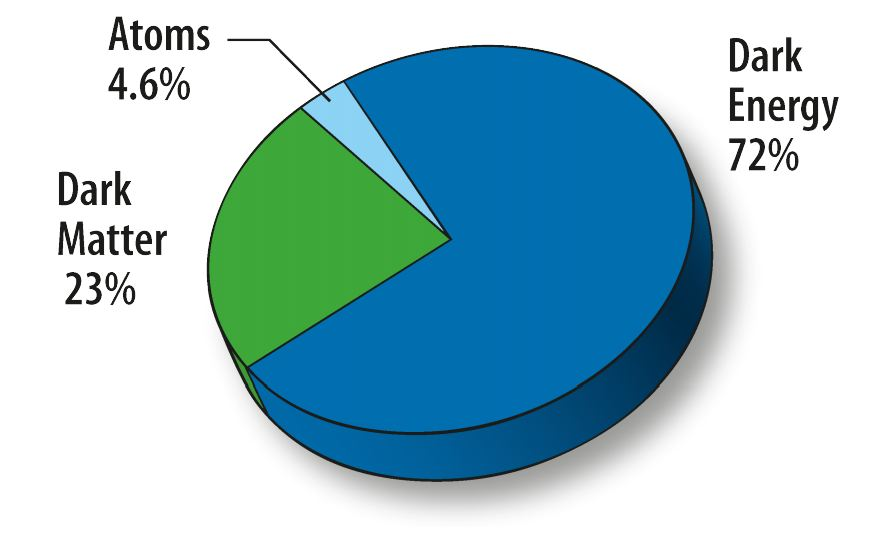
\includegraphics[width = .4\textwidth]{Pie_chart_universe.jpg}
\caption{Constituent percentages for total energy density of the universe, present day. Everyday matter (stars, interstellar gas, etc.) comprises less than 5\% of the total mass-energy density of our universe. Figure from NASA/WMAP science team, 2008 \cite{WMAP}.}
\end{figure}

\section{The $\Lambda$CDM Model of Cosmology}

The $\Lambda$CDM Model is the current, generally accepted, model for modern cosmology. This model stipulates that the universe is homogeneous and isotropic on its largest scales (on the order of gigaparsecs); conversely, if we examine the universe temporally, we see substantial differences -- an evolving universe. This evolution was shown to be an expansion, as evidenced by the redshift of distant galaxies by Edwin Hubble in the 1920s. Hubble demonstrated that our current epoch is seeing an accelerating expansion in the universe.

The conditions of isotropy and homogeneity for this model result in the Friedman-Robertson-Walker (FRW) metric,

\begin{eqnarray}
ds^2 = (cdt)^2 - R^2(t)\left(\frac{dr^2}{1-kr^2} + r^2(d\theta^2 + sin^2(\theta d \phi^2))\right)
\end{eqnarray}

where k identifies spatial curvature (either 0,-1, or +1, which corresponds to flat, negatively-curved, and positively-curved space respectively), and the parameter concerning the evolution of the universe is R(t), the scaling factor, which has dimensions of length. It is worth noting that the Hubble Constant is derived from this scaling factor: $H \equiv \frac{d log R}{dt}$.

The time evolution of this metric, and thus the universe, depends on the contents of our universe. The $\Lambda$CDM model considers three classes of mass-energy: matter, radiation, and the (relatively) recently added dark energy. Each is determined by relative values of energy density $\rho$ and relativistic pressure p. In addition, each scales differently with R(t), the scaling factor:

\begin{enumerate}
\item \textbf{Matter:} non-relativistic material whose energy density decreases as $\sim 1/R^3$ with the expansion of the universe and whose relativistic pressure $\approx 0$. This group includes baryons as well as potential cold dark matter.
\item \textbf{Radiation:} photons and relativistic matter -- such as massless neutrinos -- which have a positive relativistic pressure, and whose energy density decreases as $\sim 1/R^4$ -- faster than matter -- due to redshifts in radiation caused by expansion.
\item \textbf{Dark Energy:} an energy density present in space itself (generally known as vacuum energy) with a negative pressure, and an energy density which does not dilute with expansion of the universe. Proposed cause for the accelerated expansion of the universe.
\end{enumerate}

The inclusion of cold dark matter and dark energy are characteristic features of this cosmological model (as indicated by the name, where $\Lambda$ represents the dark energy cosmological constant, and CDM stands for "cold dark matter").

\subsection{The Density Parameter}

Another feature of the $\Lambda$CDM model is the value of the energy density, $\Omega$. This quantity comes from the Friedmann equations, which govern the expansion of space for the FRW metric. $\Omega$ describes the energy density of our universe, $\rho$, in relation to some critical energy density, $\rho_c$, for which the curvature term in the FRW metric, k, is zero. The density parameter is defined as $\Omega \equiv \rho/\rho_c$.

$\Lambda$CDM cosmology predicts that $\Omega \approx 1$, so that our universe is very nearly flat. This parameter can be separated into the relative contributions of the three classes of energy, defined as $\Omega_{x} \equiv \frac{\rho_{x}}{\rho_{c}}$  such that,
\begin{eqnarray}
\centering
\Omega = \Omega_{m} + \Omega_{r} + \Omega_{\Lambda}
\end{eqnarray}
where $\Omega_{m}$, $\Omega_{r}$, and $\Omega_{\Lambda}$ are the energy densities of matter, radiation, and dark energy respectively. This model predicts that the present energy density is dominated by $\Omega_{m}$ and $\Omega_{\Lambda}$; this arises from their different dispersion relations with the expansion of the universe. $\Omega_{m}$ can be further separated into $\Omega_{mb}$ and $\Omega_{mnb}$ which are the baryonic and non-baryonic contributions.

Experimental observations from three independent sources confirm the dominance of matter and dark energy. These are observations of distant Type 1a Supernovae(SNe), the cosmic microwave background WMAP data (CMB), and observations of baryon acoustic oscillations. Independently, each set constrains the relative energy densities weakly; however, together the data sets provide a consistent set of well- constrained energy density parameters: $\Omega_{mb} = 0.0456 \pm 0.0015$, $\Omega_{mnb} = 0.228 \pm 0.013$, and $\Omega_{\Lambda} = 0.726 \pm 0.015$ \cite{Komatsu2008}. Figure 1.2 shows the constrained parameter space of the $\Omega_{\Lambda}$ - $\Omega_{m}$ plane. Together, they dominate the total mass-energy density of the universe.

\begin{figure}[ht]
\centering
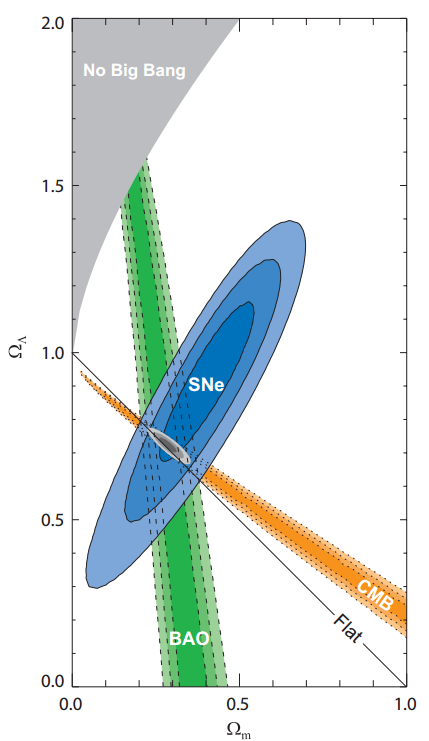
\includegraphics[width = .5\textwidth]{Energy_densities.png}
\caption{Union data for WMAP cosmic microwave background (CMB), baryon acoustic oscillations (BAO), and Type 1a supernovae data (SNe). The shaded areas show 1, 2, and 3$\sigma$ confidence regions. These data provide a consistent region in the energy density parameter space, and seem to indicate a flat universe. Figure from \cite{Kowalski2008}.}
\end{figure}

\subsection{Evolution of the Universe}
The history of our universe, as portrayed by the $\Lambda$CDM model, has some key events which will be of consequence in the sections which follow, therefore are laid out here, chronologically:
\begin{enumerate}
\item The universe originated in the Big Bang, an event which precipitated the current expansion. Before this event, all of space-time was concentrated at $R \approx 0$, in an arbitrarily small, infinitely dense region.
\item Around $10^{-36}$ seconds after the Big Bang, a period of inflation is believed to have occurred, during which the universe expanded by a factor of at least $10^{78}$. This smoothed out initial inhomogeneities, leading to the homogeneous and isotropic universe we currently live in.
\item Approximately 1 minute later, the universe cooled enough to permit fusion of protons and neutrons into the light nuclei (deuterium, helium, and lithium) in a process called Big Bang nucleosynthesis. This process was responsible for the majority of the amounts of these elements present today.
\item Nearly 400,000 years after the Big Bang, cooling had progressed enough for the first neutral atoms to form (hydrogen) from free protons and electrons in a process called recombination. Photons could now travel freely among the neutral atoms, creating a transparent universe. This initial decoupling is the cosmic microwave background we see today.
\item The next few billion years saw the formation of the non-linear structure of the universe due to small inhomogeneities which resulted in gravitational collapse to over-dense regions. Structure formation occurred hierarchically -- from small structures first, to large.
\item Around 4 billion years ago, the energy density of dark energy overtook that of matter, and the expansion of the universe began to accelerate.
\end{enumerate}

We shall see in the following section that many of these events naturally support the theory of cold dark matter.

\section{Observational Evidence for Dark Matter}

There is significant observational evidence which implies not only the existence of dark matter, but also its likely non-baryonic and non-relativistic nature. evidence can generally be divided into three main areas: the modern universe, the primordial universe, and structure formation. Evidence in the modern universe includes rotational velocities and velocity dispersions of galaxies and galaxy clusters, strong, weak, and micro gravitational lensing, and intergalactic x-ray emission spectra. The primordial universe provides us with Big Bang nucleosynthesis and the cosmic microwave background, both of which act as "baryometers" setting limits on the amount of baryonic matter in the universe. Finally, the rate of structure formation in the early universe provides further evidence of some form of non-baryonic, non-relativistic, dark matter. These will be discussed in turn below. Even at the time of this writing, techniques continue to improve, our repository of evidence grows, each time adding more support to the current theory of dark matter.

\subsection{Velocity Dispersion in Galaxies and Galactic Clusters}

In 1933, Fritz Zwicky became the first person to use the velocity dispersion within cosmological objects to infer the total mass of the system. His studies of the Coma galaxy cluster led to the conclusion that its actual mass was several hundred times higher than indicated by the amount of radiative matter. He termed this unseen matter \emph{dunkle Materie} or 'dark matter', the first reference to such a material.

The method used by Zwicky is still employed today, with great success, to characterize the mass of galaxies and clusters. For a galaxy, this process calculates the velocities of a large number of constituent stars, finding the velocity dispersion of the group. These velocities are measured through the Doppler shift of characteristic spectra, such as the 21cm HI line. The average kinetic energy can then be related to the gravitational potential through the virial theorem. This method is particularly useful for dwarf and elliptical galaxies, due to their amorphous structure. Clusters (also amorphous) are analyzed in an analogous fashion.

Recent data, particularly from the Sloan Digital Sky Survey (SDSS), has revealed numerous local, faint, dwarf galaxies which have subsequently been analyzed (see Simon and Geha \cite{Simon2007}). Their results reveal a significant dark matter dominance in dwarf galaxies, with mass to light ratios which approach 1000 times the solar mass-to-light ratio ($M_{\bigodot}/L_{\bigodot}$) in some. %explanation?

\subsection{Rotation Curves for Spiral Galaxies}

Analysis of the rotation curves for spiral galaxies also indicates a population of dark matter which -- though not as drastic as in dwarf galaxies -- is still significant. Furthermore, these curves suggest a mass distribution for the dark matter throughout the galaxies. Spiral galaxies present a particularly powerful tool for determining mass distribution, due to the simple near-circular rotational motion of their constituent stars.

A spiral galaxy is structured such that there is a central concentration of stars (the bulge) surrounded by a disc of stars. Given the rotational symmetry of this shape, if the light distribution was indicative of matter distribution, we would expect the rotation velocities -- from basic Newtonian mechanics -- to drop off as $\sim 1/\sqrt{r}$ outside the luminous galactic disk. This has been tested for a multitude of spiral galaxies, with rotational velocities calculated from line-of-sight velocities inferred from Doppler shifts of characteristic spectra: The H$\alpha$ line, the 21cm HI line, CO rotational transition lines, etc. The results, compiled by Sofue and Rubin \cite{Sofue2001}, are shown in Figure 1.3. These curves are drastically different from the behavior expected from a galaxy with most of the mass concentrated toward the center. Instead, the distribution must continue well outside of the luminous disc to allow such high rotational velocities. This is believed to be in the form of some dark matter halo, in which these galaxies are embedded.

\begin{figure}[h]
\centering
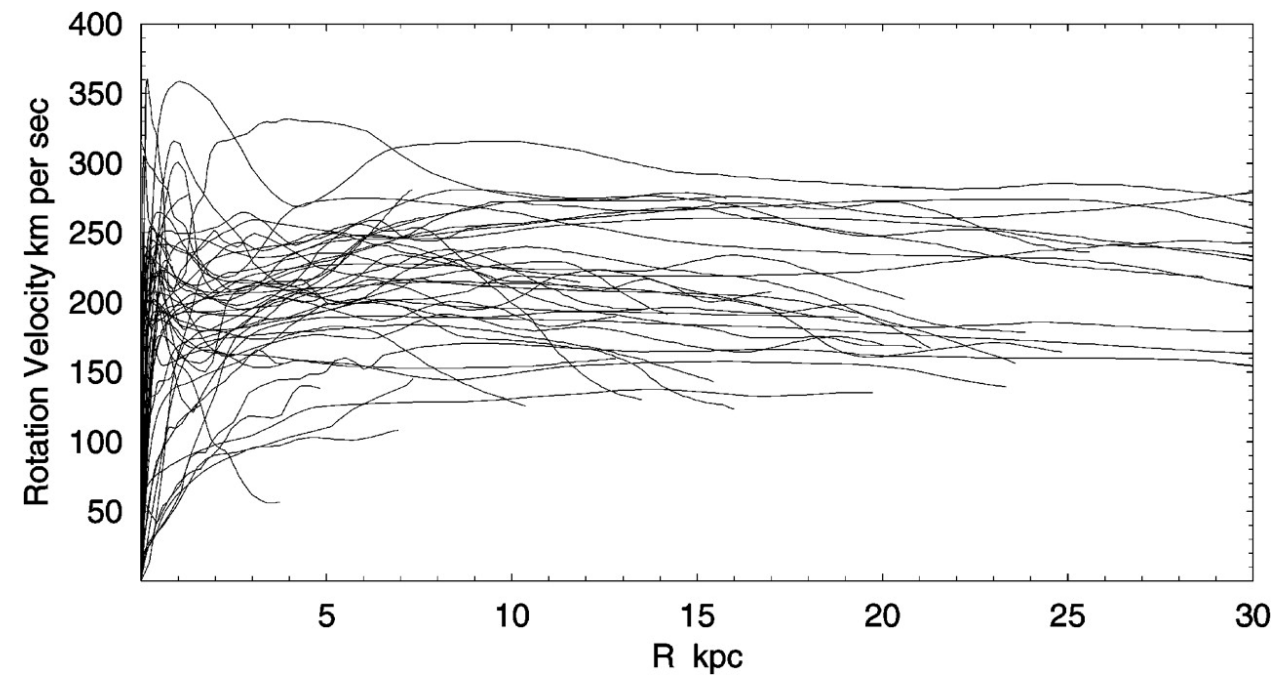
\includegraphics[width = .5\textwidth]{Rotational_velocities.png}
\caption{Aggregation of data on rotational velocities of matter as a function of distance, in kiloparsecs, from the galactic center. The flat rotational velocity curve, as opposed to one which drops off as $\sim 1/\sqrt{r}$ past the central bulge, indicates a mass distribution that extends well past the visible concentration of mass. Figure from \cite{Sofue2001}}
\end{figure}

Various methods have been developed to which are able to verify mass values obtained through velocity dispersion in clusters. One such method is observation of x-ray emission spectra from intracluster gas. Intracluster gas is superheated plasma which lies at the center of galactic clusters, and is believed to comprise up to 90\% of the total baryonic matter in a cluster. This gas is heated to temperatures of between $10^7$ and $10^8$ Kelvin by the gravitational energy of the cluster (from collision shockwaves and gravitational potential). At such temperatures, this intracluster medium (ICM) emits x-ray radiation, which determines the temperature of the ICM. If we assume that the gas is in hydrostatic equilibrium, then given a temperature profile for the ICM, we can infer the total mass of the cluster. Such observations have been made on multiple clusters up to a redshift of $z \approx 0.5$ by the \emph{Chandra} x-ray telescope, which support results obtained through velocity dispersion \cite{Vikhlinin2005,Vikhlinin2009}.

\subsection{Gravitational Lensing}

General relativity predicts that the path of light will be bent in the presence of a gravitational potential. Einstein first observed this phenomenon as the bending of starlight passing near the sun during a total solar eclipse. The same phenomenon occurs at the intergalactic scale, with the gravitational potential of the sun replaced by that of a galaxy or a cluster. This gravitational potential acts as a lens with an effective refractive index,

\begin{eqnarray}
n(x) = 1 + \frac{2}{c^2}|\Phi(x)|
\end{eqnarray}

so characterizing the path of the light allows us to determine the potential, and thus the mass of the lensing object. Figure 1.4 shows a diagram of the process of gravitational lensing.

\begin{figure}[h]
\centering
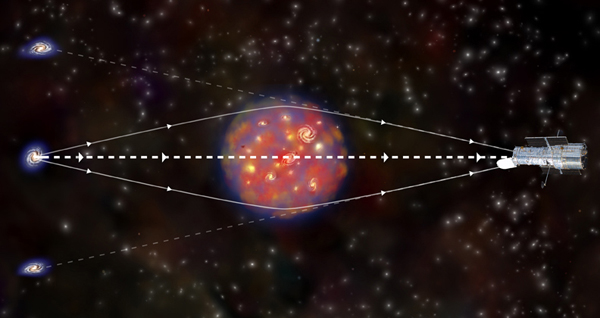
\includegraphics[width = .4\textwidth]{Lens_diagram.jpg}
\caption{Representation of the process of gravitational lensing. Light from the distant blue galaxy is refracted from the central cluster. This creates multiple images of the galaxy as shown by the faint dotted lines. Image from the Chandra X-ray Observatory website \cite{lens}.}
\end{figure}

There are three general groups of gravitational lensing:

\begin{enumerate}
\item \textbf{Strong Lensing:} Occurs when the mass density of the lensing object is high enough to produce visible distortion of background objects in the form of arcs, or full Einstein rings as in Figure 1.5. Requires near-direct alignment of observer, lensing object, and background source.
\item \textbf{Weak Lensing:} Smaller-effect lensing where the distortion of background objects must be inferred from statistical correlations among the visible shapes. Doing so allows the mass distribution of the lensing object to be determined. Far more common than strong lensing phenomena.
\item \textbf{Microlensing:} Effect caused by lensing objects of much smaller mass, such as a planet or star. Not strong enough to cause detectable distortion, but can be observed through a variation in background object brightness with the increase, maximum, then decrease of the lensing effect as the lensing object moves in front of the background object. %speak about MACHOS and micro lensing later
\end{enumerate}

Strong lensing and weak lensing are of particular importance in the theory of dark matter. They allow us to infer the total mass as well as its distribution throughout a gravitational lens. Studies of strong lensing from clusters such as Abell 2218 have led to the conclusion that there is simply not enough luminous matter to reproduce the lensing observed. Estimates for the mass-to-light ratio Abell 2218 range from 80 to 180 depending on the part of the cluster under observation, strongly supporting the presence of significant dark matter \cite{Kneib1995,Kneib1996}.

Weak lensing studies, though more difficult, have been pursued by collaborations \cite{Sheldon2009} on more than 130,000 galaxy clusters and groups. Their mass results generally agree with those obtained for the velocity dispersion methods. Furthermore, the large structure of clusters allows us to treat their properties as representative of the larger universe; by measuring $\Omega_{m}$ for these clusters, we are essentially determining $\Omega_{m}$ for the universe as a whole. Results from these studies have confirmed -- completely independently -- the value of $\Omega_{m} \approx 0.2 - 0.3$, providing support for the $\Lambda$CDM model \cite{Sheldon2009}.

\begin{figure}
    \centering
    \subfloat[]{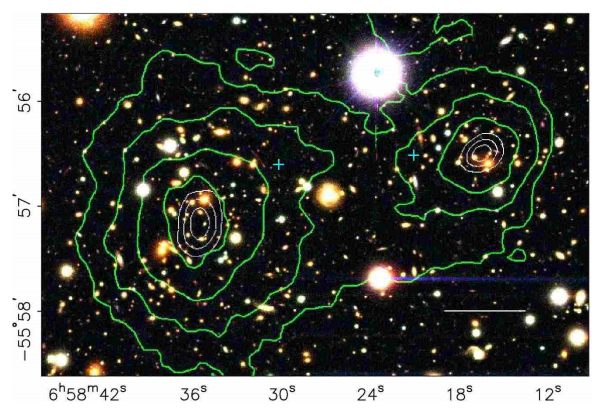
\includegraphics[width=.3\textwidth]{Bullet_visible.png}}
    \subfloat[]{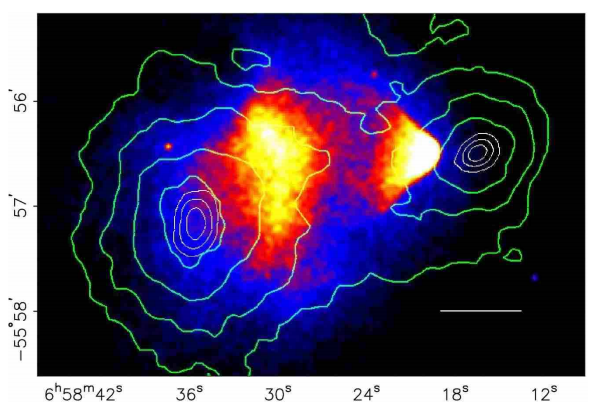
\includegraphics[width=.3\textwidth]{Bullet_xray.png}}
    \caption{Images of the Bullet Cluster, which show a clear discrepancy between the location of the baryonic matter (imaged by X-rays) and the total mass distribution. Both the visible light image (a) and the X-ray image (b) are superimposed on the mass contours inferred from weak lensing.}
\end{figure}

One of the most compelling subjects for weak lensing studies at the moment is the Bullet Cluster (1E057-558). The Bullet Cluster is actually two clusters, visible just after collision. Clowe and coauthors have analyzed the weak lensing phenomenon -- thereby constructing the mass distribution -- and compared it to the ICM distribution (which contains the majority of the baryonic matter in a cluster). The results, shown in Figure 1.6, display a substantial contrast in the distribution of the ICM and the mass contours inferred from weak lensing. We see that the majority of the clusters' mass has continued through, it did not undergo collision. These observations indicate that the majority of the clusters' mass is not only dark, but also must have a very small collision cross-section (i.e. it is non-baryonic).

\subsection{Big Bang Nucleosynthesis}

$\Lambda$CDM cosmology predicts that a period of intense nucleosynthesis occurred from roughly three minutes to twenty minutes after the Big Bang, after the universe had cooled enough to allow fusion, which created the light nuclei: deuterium ($^2H$), helium ($^3He,^4He$), and lithium ($^7Li$). The relative abundance of each of these elements depended solely on three factors: the baryon mass density, the expansion rate of universe, and the neutron-proton ratio. The last parameter, neutron-proton ratio, can be determined assuming that weak interactions at this time were in thermal equilibrium. With this, the neutron-proton number densities are $n/p = e^{-Q/T}$, where Q is the neutron-proton mass difference, and T is temperature \cite{Amsler2008}. These first two parameters can be reduced to a dependence on the ratio of baryons to photons: $\eta \equiv \eta_{b}/\eta_{\gamma}$ (photon density governs expansion rate). Photon density, however, can be determined from the temperature of the cosmic microwave background. Therefore, measuring the relic abundance of the light elements gives an accurate measurement of baryon density.

Deuterium is the most accurate "baryometer" of these light elements for two reasons. First, deuterium levels have a strong dependence on $\eta$, as shown in Figure 1.6 by the logarithmic scale used. Second, no galactic processes are currently known to exist which can produce significant amounts of deuterium. Measuring abundances of deuterium (which have not been disturbed by galactic evolution processes which can destroy deuterium) can therefore accurately determine relic deuterium abundances. Such candidates are low-metallicity stars (Population II and Population III) and low-metallicity primordial gas (ICM dubbed Lyman-$\alpha$ forests). Recent measurements of deuterium were conducted using absorption lines from high z ($\approx 3$) quasars illuminating intermediary metal-poor Lyman-$\alpha$ forests. These measurements give $\langle log(^2H/H)_{p} \rangle = -4.55 \pm 0.03$ and $\Omega_{b,0}h^2 = 0.0213 \pm 0.0010$ (68\% confidence limits) where the subscript $p$ denotes primordial abundance and $(^2H/H)$ is abundance relative to elemental hydrogen \cite{Pettini2008}. The $\Omega_{b,0}h^2$ represents the current baryonic matter portion of the critical density. The agreement between these numbers, and those found from the CMB power spectrum are shown in Figure 1.6. Their concordance lends strength to the belief that any significant presence of dark matter must be non-baryonic in nature.

The other light elements have also been used to calculate $\eta$, but due to difficulties in detection, as well as problems with post-BBN creation of these elements, results vary (see Figure 1.6). Specifically, the origin large discrepancy between the observed abundance of $^7Li$ and the predicted is a source of debate (see \cite{Amsler2008}). Though models (or theories) need to be adjusted to encompass $^7Li$, Big Bang nucleosynthesis provides strong evidence for the presence of a significant amount of non-baryonic dark matter.

\begin{SCfigure}[.7][h]
\centering
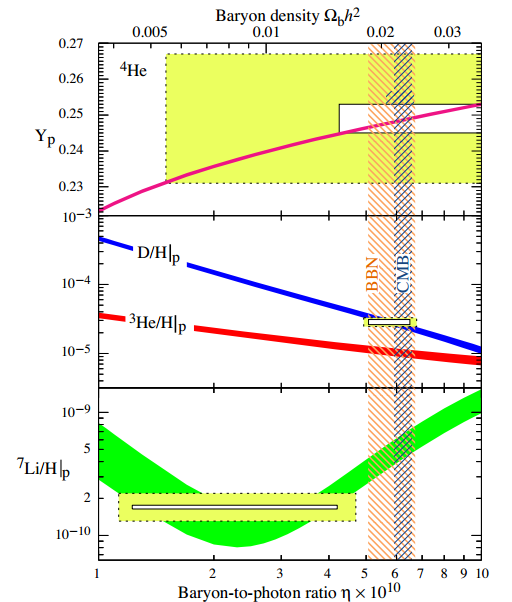
\includegraphics[width = .4\textwidth]{Deuterium.png}
\caption{Comparison of light element abundances from various sources. Curves show abundances as predicted by the standard model of Big Bang nucleosynthesis \cite{Cyburt2008} (95\% CL). The hatched vertical regions show predictions of baryon density from BBN and measurements of the CMB (also 95\% CL). The boxes show the actual observed abundances of these light elements and their agreement (or disagreement in the case of $^7Li$) with predictions;the inner boxes represent $\pm2\sigma$ statistical error, while the outer boxes are statistical and systematic errors. Figure from \cite{Amsler2008}.}
\end{SCfigure}

\begin{SCfigure}[.7][h]
\centering
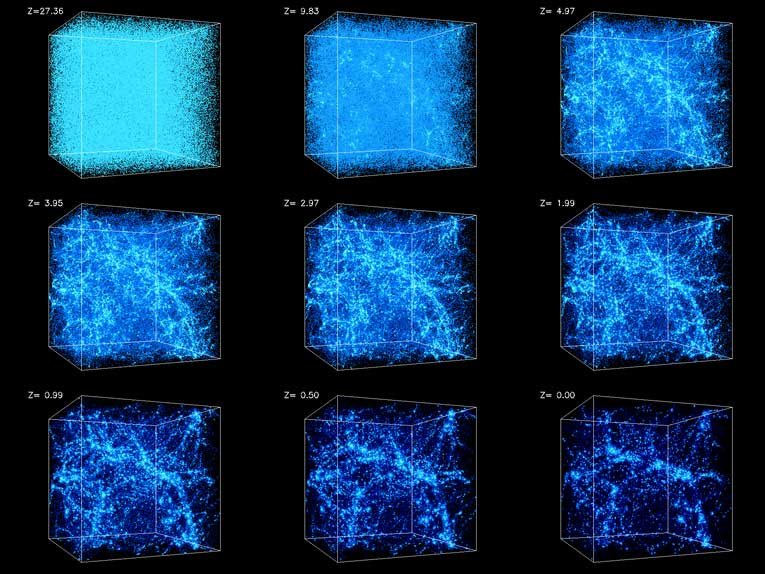
\includegraphics[width = .5\textwidth]{structure_formation.jpg}
\caption{Numerical simulations of the formation of structure in the universe from z=30 to the present over a box 43MPc in size. We see how the nearly homogeneous early universe aggregates into the overdensities to form the structure of superclusters we see today. Notice that by around z = 1, most of the structure has formed and begins to separate. Past this period dark energy dominates, which prevents further large-scale formation of structure. Figure from \cite{Simulation}.}
\end{SCfigure}

\subsection{Universal Structure}
Observations of the Cosmic Microwave Background (CMB) and other early large-scale structures present us with another set of primordial evidence which indicates significant dark matter abundance, suggests its non-baryonic nature, and requires it to be "cold" (i.e., non-relativistic at the time of the early universe).

\subsubsection{Anisotropies in the CMB}
The cosmic microwave background is an image of the early universe just after recombination. Once neutral atoms were formed, photons were decoupled from baryonic matter, and propagated through the universe. This period is called the drag epoch. The 2.73 black body radiation forming the CMB is a result of these first photons. Once photons were decoupled from baryons, baryonic matter could begin to clump into the slight matter over-densities, and begin to form large-scale structures. This process is modeled in $\Lambda$CDM by linear perturbation theory for early epochs, and numerical simulations for later periods using a relativistic theory of gravitational collapse (see \cite{Kolb1990}, \cite{Padmanabhan1993}, \cite{Liddle2000} for an explanation of the theory). Figure 1.7 shows one such simulation.

By observing the temperature anisotropies in the CMB signal (which gives photon anisotropy) we can determine baryon anisotropies at the time of the drag epoch. This is due to the tight coupling of baryons and photons prior thi epoch. These anisotropies are defined by over-densities and under-densities in the energy field,

\begin{eqnarray}
\delta(\vec{x},t) \equiv \frac{\rho(\vec{x},t) - \langle\rho(t)\rangle}{\langle\rho(t)\rangle} \\
\delta(\vec{k},t) \equiv \frac{1}{(2\pi)^{3/2}} \int \delta(\vec{x},t) e^{-\vec{k} \cdot \vec{x}} d^3 \vec{x}
\end{eqnarray}

where $\bar{\rho}(t)$ is the mean energy density of the universe at time t, and $\delta(\vec{k},t)$ the statistical distribution of the density variation for different length scales. The theory of gravitational collapse modeling the formation of structure requires these anisotropies be $\geq 10^{-3}$ at the time of recombination to allow the creation of bright galaxies as far back as $z \approx 7.6 $ \cite{Bradley2008} and the superstructures we see today. However, baryon anisotropies at similar length scales in the CMB are only observed to be $\approx 10^{-5}$. Such small anisotropies could not have formed the structures we see in similar time scales.

Dark matter provides a solution to this problem if we stipulate the existence of some \emph{non-baryonic} dark matter, as espoused by Big Bang nucleosynthesis models. This non-baryonic dark matter did not interact electromagnetically, therefore felt none of the effects of scattering photons. As a result, dark matter was able to settle into over-densities, creating gravitational potential wells long before recombination. After photon decoupling, baryons could then gravitate toward these pre-established potential wells more quickly, forming the baryon structure we see today.

\begin{SCfigure}[.7][h]
\centering
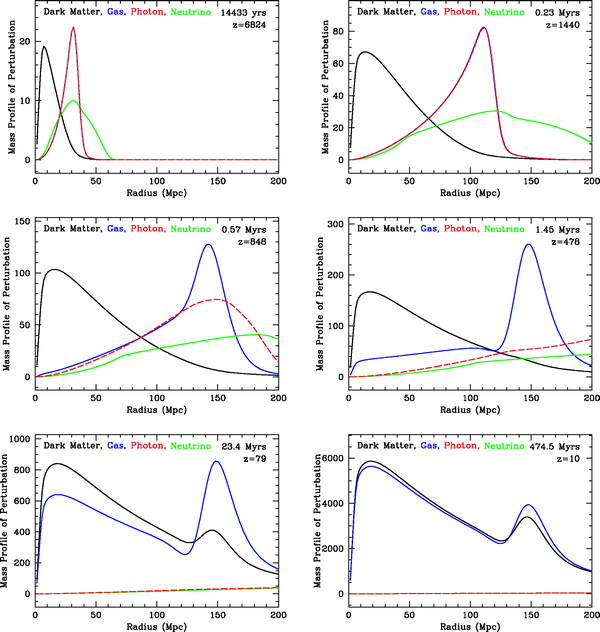
\includegraphics[width=.4\textwidth]{BAO_propagation.jpg}
\caption{Formation of baryon acoustic oscillations. Perturbations in energy density of the early universe created sound waves in the photon-baryon plasma. These waves propagated outward with photons and baryons coupled until the drag epoch freed photons and left the baryon peak stalled. This baryon peak remained as a feature in the density correlation function at $\approx 150$ MPc. Figure from \cite{Eisenstein2007}. }
\end{SCfigure}

Solving the problem of structure formation with the addition of dark matter sets another constraint on the properties any dominant dark matter candidate: it must be non-relativistic by early epochs ($z > 1000$). Relativistic matter would not have created the large potential wells required, and would not have resulted the baryon acoustic oscillations described below. Relativistic matter would have resulted in "top-down" formation of structure, where the largest structures form first. This is opposite of the hierarchical formation posited by the $\Lambda$CDM model, and does not match with observations and simulations.


\subsubsection{Baryon Acoustic Oscillations}

The argument for non-baryonic dark matter of further supported by the recent identification of baryon acoustic oscillations in large-scale structure by the Sloan Digital Sky Survey (SDSS), the 2dF Galaxy Redshift Survey (2dFGRS), and the five-year Wilkinson Microwave Anisotropy Probe (WMAP). These signatures, present in both the CMB ($z \approx 1000$) and strucures at low redshift (low z), provide powerful tools to constrain $\Omega_{m}$, $\Omega_{b}$, and $\Omega_{\Lambda}$, and offer further confirmation of $\Lambda$CDM cosmology.

Baryon acoustic oscillations, first predicted in 1970, are acoustic waves in baryonic matter which were formed in the early universe before the drag epoch. We can see the imprint left by these waves in the structure of our universe. The process (shown in Figure 1.8) is as follows \cite{Eisenstein2005}:

\begin{enumerate}
\item Over-dense dark matter regions attract baryonic matter, while photon pressure drives baryonic matter outward (dark matter, which does not interact electromagnetically, was unaffected). This perturbation excites sound waves in the photon-baryon plasma.
\item This acoustic wave travels outward at nearly half the speed of light (the speed of sound in the plasma) with the photon and baryon peak coupled.
\item Once the universe cooled enough through expansion, photons and baryons decoupled in the drag epoch. This drastically reduced the speed of sound. Photons streamed outward at the speed of light, while the baryons -- losing their driving pressure -- stalled.
\item The dark matter perturbation draws baryons back toward the center, while the baryon perturbation draws dark matter outward. This spreads the matter distribution. A peak in baryon distribution remains at the radius of the sound horizon (the baryon peak at the time of decoupling).
\item The dark matter and baryon perturbations seed formation of structure in the universe, resulting in a density correlation peak at a radius of around 150 MPc.
\end{enumerate}

Detecting the signal of these BAO is impossible without statistical analysis, as the myriad over-densities in the early universe meant creation of many interfering oscillations, which would just appear as turbulence. However, by statistical correlation measurements of over-densities, these features can be distinguished. Analysis from the five-year WMAP survey has successfully measured these oscillations as fluctuations in the power spectrum of the cosmic microwave background, placing the \emph{co-moving} sound horizon at $\sim 150$ MPc \cite{Komatsu2008}.

Whether these oscillations would still be visible in the modern universe depends on how expansion proceeded after their formation. Predictions from $\Lambda$CDM cosmology stipulate that early expansion provided linear perturbation growth. This type of growth leaves the Fourier components of the waves uncoupled, preserving well-defined features such as the sound horizon \cite{Eisenstein2005}. These features should then leave a detectable imprint on the structure of the modern universe. The Sloan Digital Sky Survey and the 2dF Galaxy Redshift Survey are the first experiments to be able to detect these faint signatures in modern matter densities. The results from the LRG (luminous red galaxy) data set in SDSS are shown in Figure 1.9. This plot shows two-point correlation function calculated for $\sim$ 46,000 galaxies at a redshift $0.16 < z < 0.47$. The sound horizon is clearly visible at a co-moving distance of roughly 150 MPc.

\begin{figure}[h]
\centering
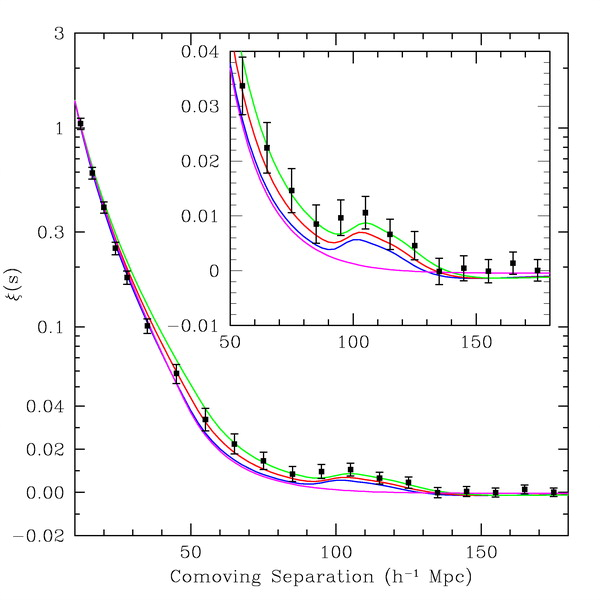
\includegraphics[width = .5\textwidth]{BAO_peak.jpg}
\caption{Correlation function found from Sloan Digital Sky Survey, LRG sample. The sound horizon, emphasized in the magnified box, is observed at $\sim 100 h^{-1} MPc$ (150 MPc). The colored lines show various cosmological parameter models: green shows $\Omega_{m}h^2 = 0.12$, red shows $\Omega_{m}h^2 = 0.13$, blue shows $\Omega_{m}h^2 = 0.14$. All assume that $\Omega_{mb}h^2 = 0.024$. The bottom pink line shows a purely dark matter curve ($\Omega_{m}h^2 = 0.105$), which lacks the peak entirely. Figure from \cite{Eisenstein2005}.}
\end{figure}

The presence and characteristics of BAO provide a wealth of information about the structure and evolution of the universe. First, the simple presence of BAO in the promordial and modern universe evidences the linear perturbation growth predicted by $\Lambda$CDM cosmology. Second, the shape of the peak provides information on $\Omega_{\Lambda}$, $\Omega_{m}$, and $\Omega_{mb}$ (baryonic matter density). The smallness of the peak in Figure 1.9 suggests a dominance of dark matter over baryonic matter, but also predicts that $\Omega_{m}h^2 \approx 0.12$ -- based on the best fit described in the figure -- leading to a dominance of dark energy in the modern universe. Third, by confirming the size of BAO at z $\sim$ 1000 and z $\approx .16$ we create a standard length scale which can tell us about the expansion of the universe, independent of supernova observations. Though the data is not accurate enough to do so at the moment, future measurements of BAO could provide a method to independently determine the Hubble parameter (H(z)) \cite{Eisenstein2005}.

Full data for WMAP, SDSS, and 2dFRGS surveys, combined with observations of distant Type1a Supernovae create the plot shown in Figure 1.2 and described in section 1.2.1. Baryon acoustic oscillations play an important role in this figure, as they provide independent measures of the cosmological parameters. Their agreement with cosmic microwave background and supernova data provides strong support for the $\Lambda$CDM model of cosmology.

\section{Candidates for Dark Matter}

The large body of evidence which supports the existence of dark matter has allowed us to infer many of its properties. The dominant dark matter in our universe must be non-baryonic, non-relativistic ("cold"), stable enough to have a lifetime which is large compared to the age of the universe, and must be nearly non-interacting. Though we have constrained many of its properties, we still must ask: \emph{what is it?}. As of this writing, this question is still unanswered, but its properties inferred from the body of indirect evidence drastically narrows the list of likely candidates. I will discuss one of the most promising members of this list, Weakly Interacting Massive Particles or WIMPs.

\subsection{WIMPs}

WIMPs (Weakly Interacting Massive Particles) are a hypothetical class of particles which interact with other matter only through weak-scale processes ("weakly interacting") and gravity. They have a hypothesized mass of $10GeV \leq M \leq 10TeV$ ("massive"). WIMPs are a favored candidate for dark matter (and the subject of our collaboration's scrutiny) not only because they would satisfy the constraints described above, but also due to cosmological considerations which predict weak-scale interaction cross-sections for dark matter particles caused by a process called "freeze out".

The full argument for the cosmological constraints on interaction cross-section for dark matter particles is beyond the scope of this chapter; however, the main argument will be reviewed here. First, the abundance of a particle in the modern universe is determined its creation and annihilation rate throughout the evolution of the universe. Figure 1.10 shows the process for determining the co-moving number density of a hypothetical particle. A particle in the early universe (just after the inflationary epoch) would be in thermal and chemical equilibrium with the primordial plasma, such that its creation from thermal production and annihilation rate were equal. The annihilation rate is given by $\Gamma$, where
\begin{eqnarray}
\Gamma = n\langle \sigma v \rangle ,
\end{eqnarray}

and $n$ is the number density of the particle, $\sigma$ is the annihilation cross-section, $v$ is the relative velocity of the two particles, and the brackets denote an average over the thermal ensemble. This rate will be equal to thermal production as long as $T >> m$, where $m$ is the mass of the particle. The number density would be constant. As T drops, thermal production stops and the number density for a massive, non-relativistic particle in thermal equilibrium after this point would be proportional to the Boltzmann constant, $n \propto e^{-\frac{mc^2}{k_bT}}$. This is shown as the solid curve in Figure 1.10. The particle would remain in thermal equilibrium until annihilation becomes inefficient, below $\Gamma \sim H$. This is known as "freeze out". The relic density after this transition is approximately \cite{Jungman1996}

\begin{eqnarray}
\Omega h^2 \approx \frac{0.1pb \cdot c}{\langle \sigma v \rangle} .
\end{eqnarray}

This can be understood generally as follows: a particle with a larger cross-section will stay in thermal equilibrium for slightly longer, resulting in a exponential suppression in the number density from the Boltzmann factor. Figure 1.10 shows expected co-moving relic densities for increasing cross-sections. From equation 1.7, to obtain relic density near that expected for dark matter ($\Omega h^2 \sim 0.1$) would require a cross section characteristic of the weak scale. Such a particle would have a mass, $m \sim 100 $ GeV.

Particle physics offers further motivation for the existence of a new particle at the weak scale. This motivation, completely independent from cosmological motivation, comes from efforts to address the "hierarchy problem" in the Standard Model (see \cite{Filippini2008} for the argument). Theories which address this problem typically call for the existence of a new particle at the weak scale. Thus, there exists strong motivation for a weakly interacting dark matter candidate. When coupled with the theoretical possibility for detection of such a particle, the allure of WIMPs as the favored dark matter candidate becomes obvious.

\section{The Cryogenic Dark Matter Search and Direct Detection}

Direct detection is the ultimate goal in determining any dark matter candidate. Indirect evidence provides us with clues as to the properties of candidates and motivates their existence, but only direct detection will allow us to confirm the existence of and fully characterize a candidate. Currently, there are roughly two dozen experiments worldwide which have engaged in the search for direct dark matter detection. These experiments use a variety of techniques in an effort for dark matter detection (see Figure 1.11).Our collaboration, CDMS, is one of the leading groups in the direct detection efforts. This section will explain the general principles governing our experiment as well give a brief history of its evolution since inception.

\begin{figure}[h]
\centering
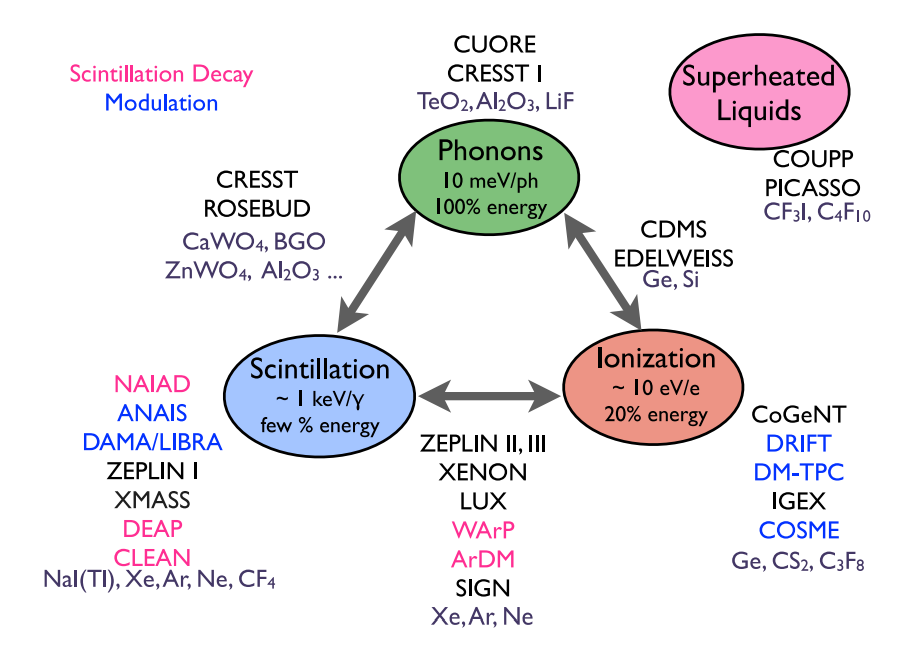
\includegraphics[width = .5\textwidth]{Dm_experiments.png}
\caption{Different detection methods utilized by dark matter experiments. The CDMS Experiment uses phonons and ionization for improved background rejection. Figure from \cite{Figueroa2011}.}
\end{figure}

The CDMS Experiment has been taking data in low background environments since 1996. In the years since then, the experiment has gone through several iterations: CDMS I, CDMS II, SuperCDMS Soudan, and SuperCDMS SNOLAB (currently under development). Detection technology has changed significantly, but the basic principle remains the same: that WIMPs will scatter elastically off nuclei in atoms, producing a signal which can be detected as energy deposition. This energy deposition can be characterized through the collection of phonons and charge from interaction recoils. Characterizing each "event" (nuclear or electron recoil in the detector) allows us to discriminate possible WIMP interactions from background.

\subsection{Background}

For our experiment, background is anything that could be misconstrued as a WIMP interaction. The major background in our experiment consists of $\beta$, $\alpha$, $\gamma$ radiation, as well as neutrons and cosmic ray muons. These background events can occur at a rate of $ \sim 10^{13}$ times that for predicted WIMP events, therefore extensive measures are taken to reduce their occurance.

The experiment uses multiple stages of shielding to drastically lower this background:
\begin{enumerate}
\item \textbf{Underground:} experiment location determines muon flux. CDMS I was located at the Stanford Underground Facility (SUF) which provided shielding of 16 meters water equivalent (mwe). This reduced the observed muon flux by a factor of 5 \cite{Abusaidi2000}. CDMS II moved to the Soudan mine in Minnesota which provides $\sim 2100$ mwe. SuperCDMS SNOLAB will move to the SNOLAB facility (at the Sudbury mine in Ontario Canada) which provides $\sim 6000$ mwe shielding. These depths greatly reduce muon flux as well as cosmic ray gammas (a factor of $\sim 1000$ from Soudan to SNOLAB facility \cite{Saab2012}.
\item \textbf{Active veto:} To further mitigate the muon background, a muon scintillator surrounds the experiment. This detects muons and can rule out muon coincident events in the detector (rendered unnecessary in SNOLAB).
\item \textbf{Polyethylene:} A circular shield of polyethylene is placed inside the active veto to moderate neutrons produced by muons interacting with the active veto.
\item \textbf{Lead:} 23cm of lead shields the experiment from external gammas.
\item \textbf{Ancient Lead:} A layer of low activity lead (obtained from a Roman shipwreck) shields betas from the outer lead.
\item \textbf{Polyethylene:} A final layer of polyethylene shields the experiment from the ancient lead.
\item \textbf{Radiopure Experiment:} Finally, all of the materials used inside of the dilution fridge containing the experiment are selected for extreme radiopurity to prevent \emph{production} of any background in the experiment. In addition, care must be taken to prevent activation of any materials from cosmic rays.
\end{enumerate}

After these extensive measures are taken to minimize background, we are still left with $\sim 1$ event/kg/KeV/day \cite{Saab2012}. Methods must then be developed to distinguish these background events from possible WIMP signals, as discussed below.

\subsection{Basic Detection Method}

The detection methods used in the CDMS experiment are phonon and ionization signals. These methods use an ultra-pure (as low as $10^{13}$ impurities/$cm^3$) single-crystal semiconductor material such as Germanium or Silicon cooled to $\sim 20$ mK in a dilution fridge. These extreme temperatures are necessary to limit thermal noise present and thus increase sensitivity to particle collisions with the detector lattice. When a particle collides with the lattice, two things happen:
\begin{itemize}
\item Free electron/hole pairs are created due to the semiconductor nature of the detector. These charges can be collected by applying a voltage across the detector.
\item Athermal phonons are excited in the lattice, which can be detected through various means.
\end{itemize}

These two methods of detection provide a powerful tool for discerning between possible WIMP interactions and background events which penetrate to the detector. This is because most background particles interact with atomic electrons (electron recoil). Only neutrons and WIMPs interact with the nucleus of an atom (nuclear recoil). These recoils deposit energy through ionization and phonon production differently. These differences can be described by the ionization yield, Y, which is the ratio of energy deposited through ionization to the amount deposited as phonons. Electron recoil typically has Y$\sim$1 while nuclear recoil has nuclear recoil has a Y$\sim$0.3. Since background is heavily dominated by electron recoil interactions, this method is very useful for background rejection.

Below, a brief description of each generation of the experiment highlighting technological improvements is presented.

\subsection{CDMS I}
The first experiment used two detector types: BLIP (Berkeley Large Ionization- and Phonon-based) and FLIP (Fast Large Ionization- and Phonon-based) detectors. BLIPs used neutron transmutation doped Ge thermistors (NTD) bonded to Ge crystals. These collected phonon energy through a calorimetric temperature change in the crystal. FLIPs, on the other hand, used W QETs for phonon collection. BLIPs were germanium detectors, while FLIPs were either germanium or silicon. Germanium was ultimately adopted in later experiments due to the larger nucleus which improved probability of nuclear recoil. Both technologies used JFET ionization sensors on one side which received charges through a voltage established across the bulk of the detectors.

\subsubsection{W QETs}

W QETs (Tungsten Quasiparticle-trap-assisted Electro-thermal-feedback Transition-edge-sensors) use aluminum pads lithographically patterned on one surface of the detectors with an array of tungsten wires attached to them. The tungsten wire is held near its superconducting transition temperature ($\sim$ 80 mK). The superconducting aluminum pads cause phonons to deposit energy as heat. This heat causes an abrupt transition in the tungsten, whose change in resistivity is detected as a current pulse in a SQUID amplification array. This method allowed for a factor of 10 better sensitivity in phonon detection, as well as X-Y localization of the event to within a few millimeters \cite{Gaitskell1997}.


\begin{figure}[h]
\begin{centering}
\subfloat[Left side shows four phonon channels, while right shows two charge channels.]
  {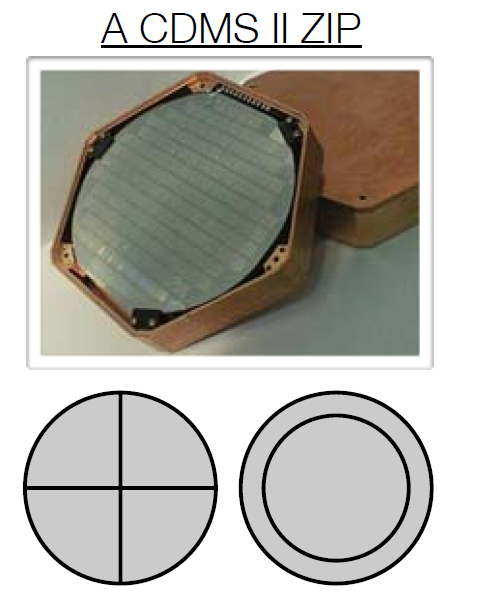
\includegraphics[width=0.3\textwidth]{ZIP.png}}
  \hspace{10pt}
  \subfloat[iZIP detectors have four phonon channels and two charge channels on each side.]
  {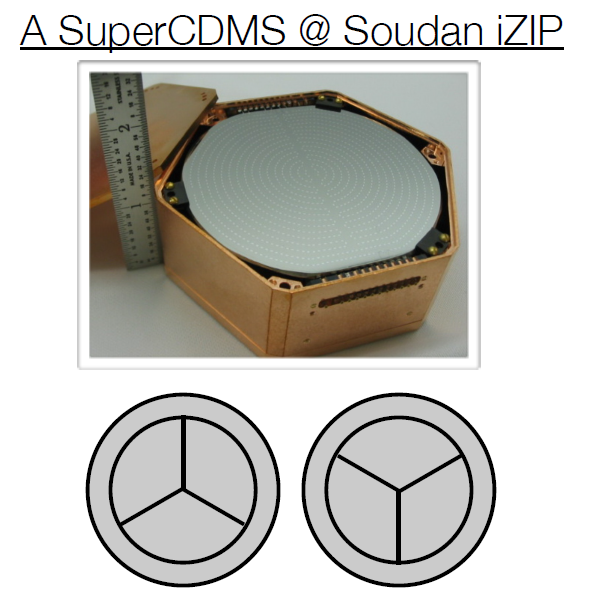
\includegraphics[width=0.3\textwidth]{iZIP.png}}
  \subfloat[SNOLAB detectors will have six phonon channels and two charge channels on each side.]
  {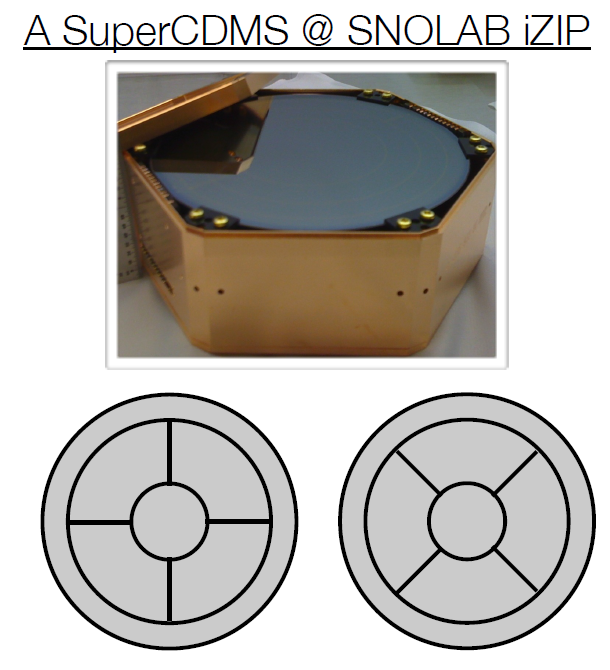
\includegraphics[width=0.3\textwidth]{iZIP_snolab.png}}
\caption{Detector layout for CDMS experiments. Pictures from \cite{Saab2012}.}
\end{centering}
\end{figure}

\subsection{CDMS II}

CDMS II was located in the Soudan mine, which drastically reduced cosmic ray background. This is important, especially for muon flux, as muons can produce neutrons in materials. This neutron background is significantly more difficult to distinguish from possible WIMP interactions than other types of background, as it produces nuclear recoil rather than electron recoil. Another major improvement was the development of ZIP (Z-sensitive Ionization- and Phonon-based) detectors. ZIPs had four phonon channels on one side and two charge collection channels on the other side of the detector. Figure 1.11 a) shows the layout of the phonon and charge channels for the ZIP detectors. These detectors built upon the FLIP technology in CDMS, and by creating four phonon channels allowed further localization of events. Combined with ionization yield, this increased electron recoil rejection to $> 10^{-6}$ (only 1 in $10^6$ electron recoil events would be mistaken for a WIMP signal) \cite{Saab2012}.

\subsection{SuperCDMS Soudan}

The next generation of the experiment greatly improved detector technology with iZIPs -- where the "i" stands for interleaved. This germanium detector has four phonon channels and 2 charge channels on \emph{each side} as can be seen in Figure 1.11 b). The layout not only provides localization improvements (e.g. unambiguous radial positioning of events \cite{DOE}) but also addresses the largest source of background for the CDMS II experiment: leakage events \cite{Akerib2005}.

\begin{figure}[h]
\centering
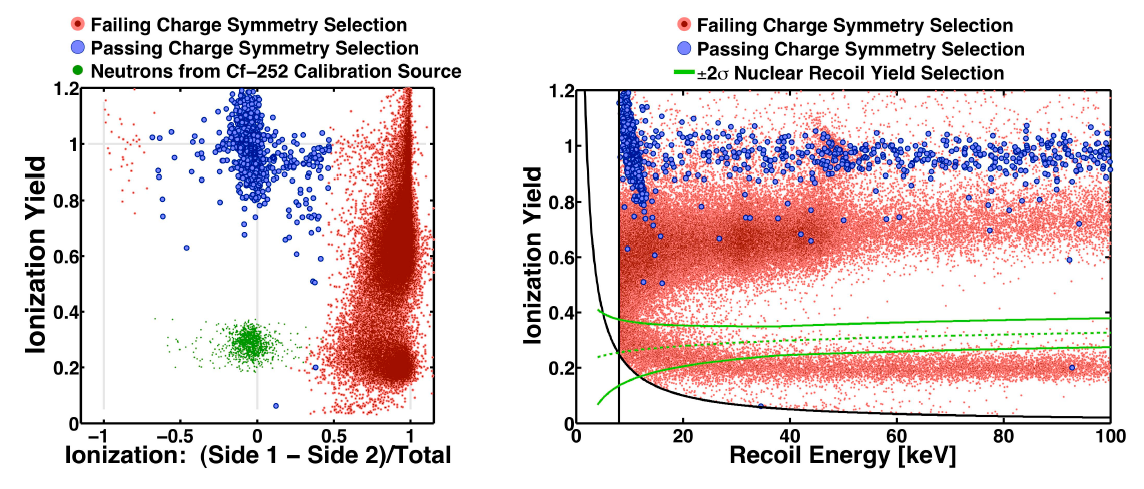
\includegraphics[width = .8\textwidth]{iZIP_ionization.png}
\caption{Utilization of iZIP symmetry conditions to reject surface "leakage" events. These events occur close enough to the surface so that charge is only collected on one side, breaking symmetric charge collection.}
\end{figure}

\subsubsection{Leakage events}

These leakage events are electron recoil interactions which occur in the "dead zone" of the detectors (near the surface) where charge collection efficiency is lower. This produces low ionization yields which "leak" into the nuclear recoil regime of the signal, as shown in Figure 1.12 on the right plot. The lowest electron recoils overlap with the nuclear recoil regime, where they can be mistaken for nuclear recoils. By locating charge channels on both sides and establishing a voltage difference between charge and phonon channels, an electric field is produces such that electron recoils that occur within $\sim$ 1 mm of the surface are only collected on one side. This distinguishes the low ionization electron recoils from symmetric charge collection nuclear recoils. Symmetry selection now allows us to rule these events out with a rejection of $10^{-5}$ \cite{Saab2012}.

\subsection{SuperCDMS SNOLAB}

The next generation CDMS experiment will take place in the Sudbury mine in Ontario, Canada. This mine is nearly three times as deep as Soudan, which will render the muon flux negligible. Furthermore, the design of the detector will change once more so that it is larger, with six phonon channels and two charge channels on each side, as seen in Figure 1.11 c), which leads to a further increase in signal sensitivity and improves rejection of backgrounds. Additionally, we will be using HEMTs (High-electron-mobility transistors) instead of FETs as low-noise amplifiers. This provides a huge reduction in power dissipation to the tower, as FETs must be heated to 100K to operate (they freeze out below this temperature. Another advancement in the experiment is the consideration of an active neutron veto, which is estimated to be capable of rejecting 79\% of all neutron-induced backgrounds \cite{DOE}. In addition, this experiment will be a massive upscaling in detector mass (around 200kg as compared to $\sim$10 kg for previous experiments). Figure 1.13 shows the projected upper limit of $\sigma \approx 8 \cdot 10^{-47} cm^2$ for the spin-independent cross section for SuperCDMS SNOLAB in comparison to results from previous experiments.

\begin{figure}[h]
\centering
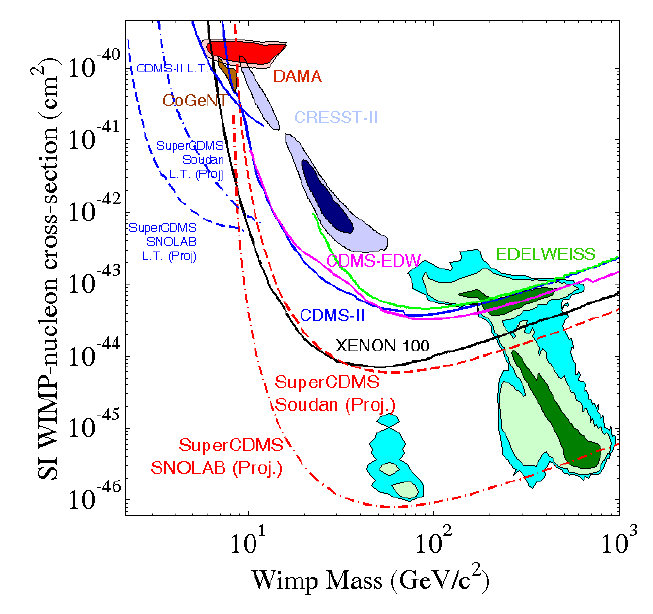
\includegraphics[width = .5\textwidth]{crosssection.png}
\caption{Upper limits on the spin-independent cross-section and WIMP mass parameter space as set by various dark matter experiments. The dash-dot line shows the projected upper limits for SuperCDMS SNOLAB due the the large detector payload (200kg) and increased detector. Figure from \cite{DOE}.}
\end{figure}

\chapter{SuperCDMS Soudan Tower}

This brief chapter discusses the design of the current tower in order to determine the design aspects we must consider in the SuperCDMS SNOLAB tower. These include the considerations for the charge and phonon read-out lines and the tower thermal stand-off tubes, which are being substantially re-designed for the new SuperCDMS SNOLAB. A model of the current tower -- with the detector stack mounts -- is shown in Figure 2.1. This is the tower currently in use for the SuperCDMS Soudan experiment. The various components of the tower are described below, along with their design considerations.

\section{Tower Floor}
The bulk of the tower is made of OFHC (Oxygen-Free High Conductivity) Copper. This was chosen for its high thermal conductivity, dimensional stability, and high radio-purity. High thermal conductivity is required to ensure that the tower floors (and all devices heat sunk to them) are as close to the fridge stage temperatures as possible. Dimensional stability plays an important role during the cooldown of the experiment. If the tower's thermal contraction is too large, differential contraction can lead to either slack in the side-coaxes or stresses which can lead to thermal fatigue over multiple fridge run cycles. Lastly, a high radiopurity is required for all materials in the tower to minimize potential background in the experiment during operation.


\section{Heat Sinks to Dilution Fridge}

Excellent thermal links to each temperature stage of the fridge are necessary in order to maintain constant temperatures on the tower and enable effective heat dissipation. To achieve this, the current tower uses OFHC copper straps. These are composed of dozens of braided strands of well-annealed copper (RRR = 1200) which provide a large enough cross-section of copper to dissipate heat, but maintain flexibility to prevent stresses from being created at the heat strap mount points \cite{Stockwell1996}.


\section{Tower Thermal Stand-offs}

The thermal stand-offs in the tower serve to thermally isolate each stage of the tower, while physically connecting the tower stages. The current experiment uses thin-walled graphite tubes between each stage, visible in Figure 2.1. These are nuclear-grade UF-4S graphite purchased from Mersen, milled to an OD of 1.99" and 0.028" wall thickness. Apart from the wiring, these are the only structures which make inter-stage connections. The design of these is crucial, and comes from the intersection of numerous constraints: stiffness requirements, thermal loading limits, dimensional stability, radiopurity, and mechanical strength.

\begin{figure}[h]
\centering
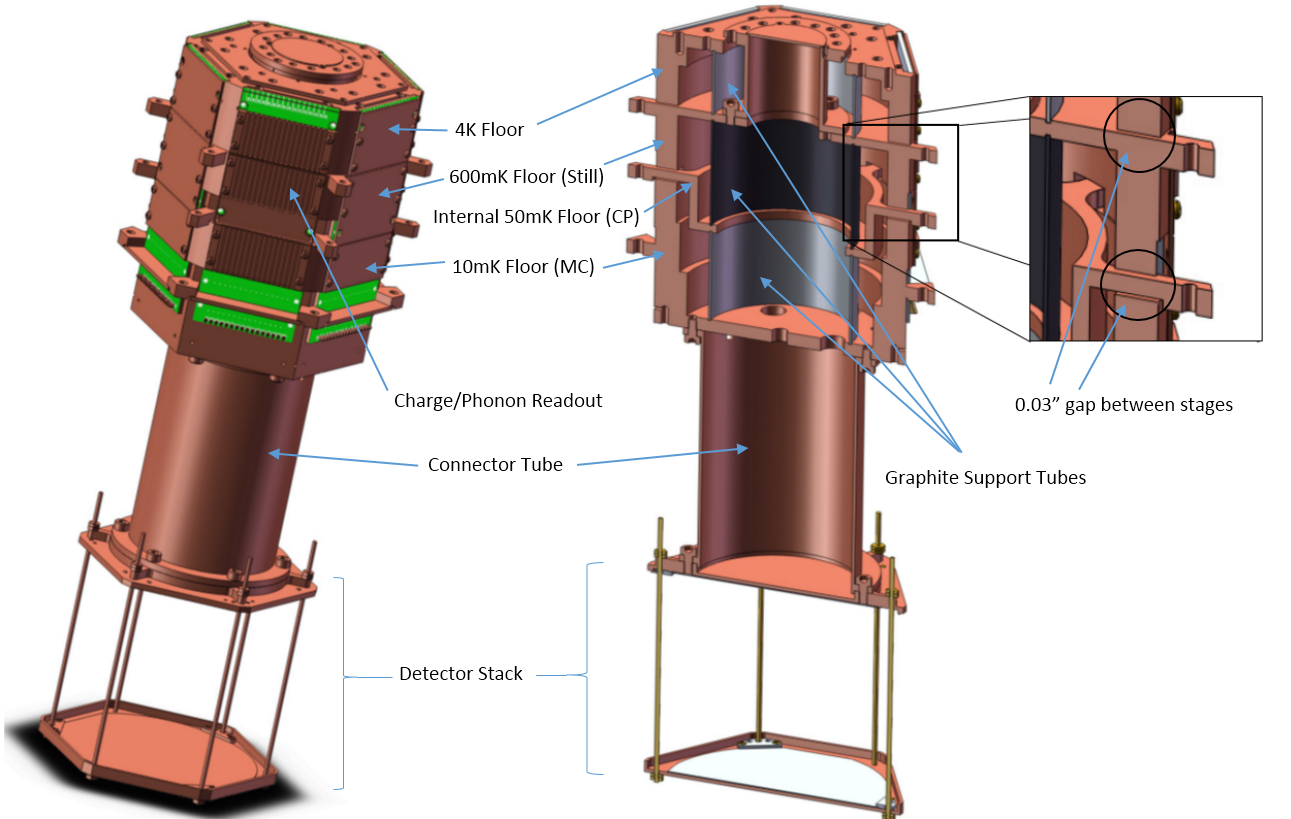
\includegraphics[width = .75\textwidth]{Labelled_tower.png}
\caption{Model of the SuperCDMS Soudan towers currently in use. The graphite support tubes and vacuum coax lines for charge/phonon readout are visible. The different thermal stages, which are thermally linked to the fridge, are visible in both models. These are 4K, 600mK (Still), 50mK (Cold Plate), 10mK (Mixing Chamber). Note that the 50mK stage is internal to the tower.}
\end{figure}

\subsection{Stiffness and Dimensional Stability}
The constraints on stiffness and dimensional stability stem from the requirement that the stage spacing doesn't change significantly during fridge operation. This is for two reasons: First, it ensures correct operation and preservation of the vacuum coaxes. A tower which isn't sufficiently stiff can deform during handling, which could potentially damage the coaxes. A coefficient of thermal contraction which is too high can either create slack in the vacuum coaxes (shorting them to the tower) or cause stresses in the wires, which could plastically deform them \footnotemark. \footnotetext{see Appendix A for an investigation of stresses experienced by the NbTi vacuum coaxes which suggest large enough stresses to potentially result in plastic deformation.} Second, a low coefficient of thermal contraction for the stand-offs ensures that the different tower stages don't come into contact during cooling, which would create a thermal short between fridge stages\footnotemark. Graphite has very high dimensional stability, as well as a high enough modulus of elasticity to ensure a stable tower during cooldown and handling.

\footnotetext{This is not a concern for the new tower, which features a more open design and much larger stage separation.}

\subsection{Radiopurity}
The requirement for radiopurity in the thermal stand-offs come from the need to minimize background for our experiment. This is especially important for materials which are near the detectors, as there is little to no shielding to block radiation. The graphite in use is a nuclear grade graphite (very low impurity), which was shown to be very radioactively "clean" through a screening process.

\subsection{Thermal Isolation}
One of the largest requirements of the thermal stand-offs is that they are very good insulators (low thermal conductivity) in order to ensure that heat flow between adjacent thermal stages of the tower is minimal. The UF-4S graphite used was shown to have very low thermal conductivity, so satisfied this requirement nicely.

\subsection{Mechanical Strength}
The tower supports were designed to be strong enough to withstand varied loads during handling and operation. This includes lifting/tilting the tower and supporting the detector stack in compression when mounted in the fridge. The symmetric tube shape of the supports ensures strength for many types of loads, and was proven to be very strong (it could support over 125lbs when loaded in shear/bending!).


\section{Vacuum Coaxes}
Wiring must be routed down the side of the tower to the detector stack in order to control the detectors and read them out. The current design uses vacuum coaxes. These consist of .0012" diameter niobium-titanium (NbTi) wires suspended in rectangular grooves in the tower faces, which act as shielding. The grooves which encase each suspended wire are visible in the left image in Figure 2.1.

The vacuum coaxes were chosen for multiple reasons: First, they offer very low noise pick-up. This is critical when the signals being read-out from the detectors are so small. Second, they prevent any charge build-up (?). Third, they minimize heat conduction between stages, because the bare NbTi wires are the only connection which is contiguous between all stages. This, in conjunction with the very low thermal conductivity of NbTi, provides very low heat conduction. Lastly, NbTi wires are superconducting below approximately 10K, which gives us zero resistance wiring to minimize signal loss before amplification.

\section{Connector Tube}
The tower connector tube is a cylindrical OFHC Copper tube which connects -- both physically and thermally -- the 10mK floor to the detectors. The purpose of this tube is two-fold: First, it roughly centers the detectors in the icebox of the fridge. This simplifies Monte Carlo simulations of detector performance. Second, it distances the radioactivity-sensitive detectors from the tower materials, which may be more radioactive than other materials in the experiment. Increasing the distance to the tower decreases the solid angle that the detectors subtend from the tower's position, which decreases the probability that an emitted radioactive particle will strike the detectors.

\section{Thermal Load Contributions for SuperCDMS Soudan}

To determine
\section{Future Tower Considerations}
Though the design and technology used will change for the SNOLAB tower, many of the considerations which went into designing the SuperCDMS Soudan tower will remain into the new design. As shown above, these considerations are numerous, and often competing (such as maximizing support strength while minimizing thermal conduction). Moving forward with the new tower design, these considerations should be kept in mind.


\chapter{Tower Thermal Stand-off Design}

As stated in the previous chapter, the thermal stand-offs for our detector tower are designed primarily to support the detector stack and electronics, while thermally isolating the various 4He-3He dilution fridge temperature stages. However, any tower support structure must address numerous concerns in its design; These concerns are: thermal conductivity, radiopurity, thermo-mechanical properties such as strength, moduli, and expansion coefficients, and -- for the design of the structure itself -- the ability to withstand various loads and shocks without failure. In this chapter, I explore various stand-off candidates which offer significant improvements over our current UF-4S graphite tubes based on their merits of thermal conductivity, radiopurity, and their thermo-mechanical properties. From here, I consider two design possibilities for the stand-off geometry: thin-walled cylindrical shells and hexapods. An analytical model for the thin-walled shells -- or "tubes" -- is developed in an effort to further improve fridge performance by optimizing tube dimensions to minimize heat load while maximizing strength. An FEA modeling program called Comsol is then used to analyze both the tube and hexapod structures. We find that new designs for SuperCDMS SNOLAB may be able to reduce interstage heat loads from the thermal stand-offs by almost a factor of ten.

\section{Candidate Materials}
The numerous parameters which our thermal stand-off materials must satisfy gives us a list of equally numerous candidate materials, each of which is known -- or believed -- to satisfy at least some of the requirements (that they satisfy other requirements is proven in the following sections). This section identifies the various candidates and describes their merits as stand-off materials.

\subsection{DuPont Vespel}
Vespel is a polyimide-based material produced by DuPont which is widely used in both high-temperature, and cryogenic applications. The polyimide is a condensation type produced from pyromellitic dianhydride (PMDA) and 4,4' diamino diphenyl ether (ODA)\footnotemark. We are considering four compounds of Vespel for this experiment: SP-1,SP-22,SCP-5000, and SCP-5050. The SP-series compounds are estimated to have a crystallinity of between 25 and 50\%.

\footnotetext{Information from DuPont literature: Vespel S line Design Handbook}

Vespel SP-1 is the unfilled polyimide resin. This compound has low thermal conductivity, is high strength, and has demonstrated low levels of radioactivity. SP-1 has a low dimensional stability, however, with a high coefficient of thermal expansion (CTE) an low elastic moduli.

Vespel SP-22 is the base polyimide, SP-1, filled with 40\% graphite by weight. This material is even lower thermal conductivity than SP-1, making it an ideal candidate. In addition it offers higher dimensional stability than SP-1, with a lower CTE and higher moduli of elasticity. Unfortunately, it demonstrates a high level of radioactivity which probably originates from the graphite used.

Vespel SCP-5000 is an unfilled polyimide resin very similar to SP-1, however it has been engineered to have higher strength and improved dimensional stability. This includes a lower CTE and significantly higher elastic moduli. At the same time, we have shown that SCP-5000 has a thermal conductivity as low as SP-1.

Vespel SCP-5050 is analogous to SP-22 in that its composition is base resin (SCP-5000) filled with 40\% graphite by weight. It is not as strong as SCP-5050, but offers the highest dimensional stability of the Vespel compounds being considered; its CTE is designed to be similar to steel. In addition, it demonstrates a lower radioactivity and lower thermal conductivity than SP-22.

All the Vespel compounds are being considered as isostatically formed parts, rather than direct formed, because this ensures isotropic structure and properties. Direct formed parts are created with a process similar to powder metallurgy, which leaves them with anisotropies. This has consequences for the material properties, such as a tensile strength and elongation which are lower in the direction parallel to the moulding force.

\subsection{Graphite}

Our current thermal stand-off material, grade UF-4S from Mersen, is graphite for many reasons. Graphite is known to have a very low thermal conductivity, and high dimensional stability. Its radioactivity can be minimized by purchasing nuclear grades, or by purification processes such as the one described in section 3.3.2 which reduce radioactive contaminants to very low levels.

The first graphite candidate is Grade 2020 from Mersen. This material was recommended to us by the R\&D manager at Mersen for low thermal conductivity and high strength/purity. It is a nuclear grade graphite which can be further purified, and demonstrates reasonable radioactivity levels. It has a high dimensional stability, and is stronger than UF-4S graphite.
The next graphite grade being considered is AXM-5Q\footnotemark, an industrial grade graphite produced by POCO. This material exhibits even lower thermal conductivity than UF-4S graphite (section 3.2) and higher strength. Off the shelf, this material displays very high levels of radioactivity compared to what our experiment can tolerate. However, purification offers a way to reduce these levels to well within our tolerated limits. In addition, it has a small grain size (5 microns) which gives it high isotropy.

\footnotetext{In addition to grade AXM-5Q, we have also considered grades ZXF-5Q and ACF-10Q. They are both industrial grade graphite offered by POCO. Apart from counting their radioactivity, however, little research has been done into their properties, therefore they are not discussed as a likely candidate.}

\subsection{TiMetal Titanium Alloys}

TiMetal produces two titanium alloys which are currently of interest to us: Ti 15-3-3-3 and Ti 21s.

Ti 15-3-3-3, also known as Ti 15V-3Al-3Cr-3Sn or simply Ti 15-3, is a meta-stable $\beta$-alloy of titanium. It is a superconductor at low temperatures, has low thermal conductivity, and high strength and elastic moduli. Screening has also shown it to be low radioactivity. The issue with this alloy is that true TiMetal Ti 15-3-3-3 is only available in sheets or as a foil. Ti 21s is another meta-stable $\beta$ alloy manufactured by TiMetal. It has good mechnical properties -- high strength and elastic moduli -- but its other properties are not known. It is being considered as a stand-off material in the hopes that it has interesting properties, similar to Ti 15-3-3-3.

\section{Thermal Conductivity}
Due to the finite cooling power of our helium dilution refrigerator, we must limit the
thermal load to each stage of the fridge. The tower support tubes are a major source of
thermal loading on each stage. The thermal power load on each stage from the tubes is
governed by the general equation
\begin{eqnarray}
Power = \int_{T_{low}}^{T_{high}} \frac{A}{L}K(T)dT \ \ , %place this above in a more general section and reference it.
\end{eqnarray}
where $T_{low}$ is the temperature of the colder stage (the one being thermally loaded), $T_{high}$ is the warmer
connecting stage, A is the tube cross-sectional area, L is tube length, and K(T) is the temperature-dependent
thermal conductivity. From the equation, we can see that thermal power is directly proportional
to thermal conductivity, so by decreasing thermal conductivity, we decrease power to each
stage; therefore, a first-pass look at tower material candidates should search for those materials which have a low thermal conductivity. These candidates are shown in comparison to the material currently in use -- UF-4S Graphite -- in Figure 3.1 below.
\begin{figure}[htb]
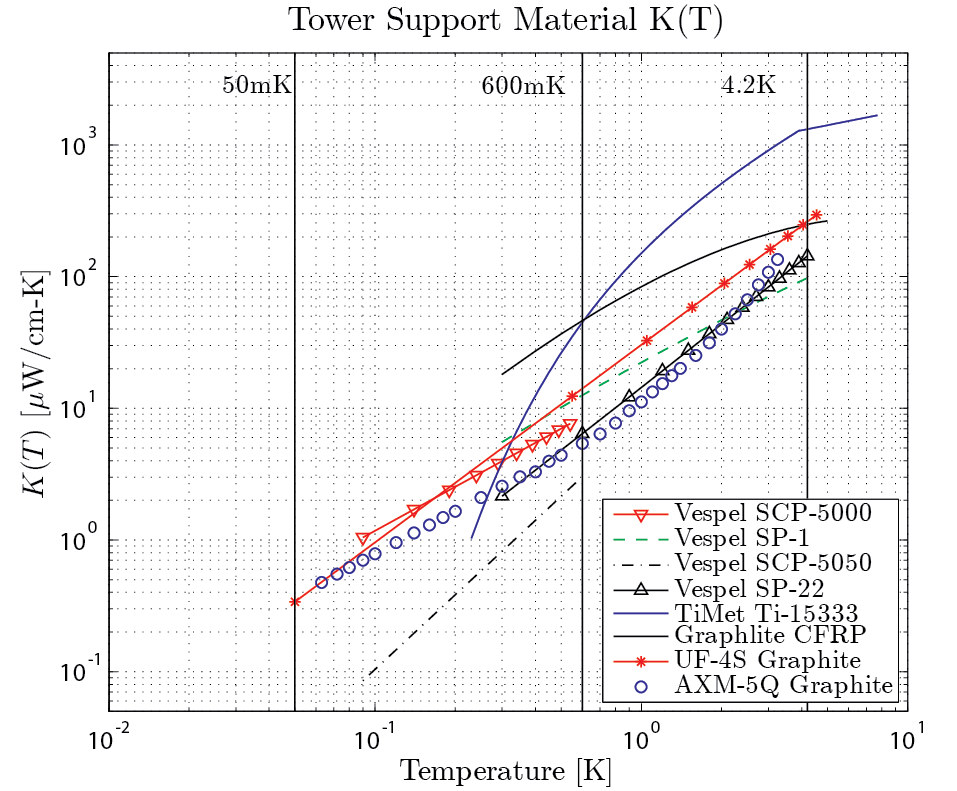
\includegraphics[width = \textwidth]{C:/Users/Niko/Documents/LaTex/Nick_K_Thesis/CH3_figs/Standoff_K.png}
\caption{Thermal conductivity of candidate tower stand-off materials. These data were collected from multiple papers: Vespel SCP-5000 \& Vespel SCP-5050 - This work ; Vespel SP-1, Vespel SP-22, Graphlite CFRP - \cite{run} ; Ti 15-3-3-3 - \cite{wik} ; UF-4S Graphite - \cite{lem} ; AXM-5Q Graphite - \cite{woo:gr}.}
\end{figure}



Table 1 summarizes the possible improvements in thermal power conducted for each stage,
assuming identical tube dimensions.

\begin{table}[htb]
\begin{threeparttable}
{\footnotesize\rm\begin{tabularx}{17.7cm}{l|XXXXXX}
  \multicolumn{7}{l}{{\large Calculated Power Conducted for Candidate Tower Materials}}\\
\toprule
 {\normalsize Material} & 4.2K-600mK  &5K-1K\tnote{*}& 600mK-50mK & 1K-100mK\tnote{*} & 50mK-10mK & 100mK-40mK\tnote{*} \\
  &P($\mu$W)&P($\mu$W)&P($\mu$W)&P($\mu$W)& P(nW) & P(nW) \\ \hline\hline
  Current Graphite & 202 & 309 & 0.95 & 3.4 & 2.2 & 11.4 \\
  POCO AXM-5Q & 140 & 238.4 & 0.46 & \textbf{1.35} & 2.75 & 10.5 \\
  Ti-6Al-4V 'Grade 5' & 2294 & 3490 & 7.8 & 43.6 & 0.4-2.13 & 6.4-21.1 \\
  Ti 15V-3Cr-3Sn-3Al & 1134 & 1623 & 1.79 & 12.4 & - & - \\
  45Nb-Ti (45\% wt. Nb) & 1715 & 2879 & 3.0 & 13.9 & 2.1 & 15.5 \\
  Vespel SP-1 & \textbf{92.2} & \textbf{129} & 0.96 & 2.92 & 4.9 & 19.8 \\
  Vespel SP-22 & 107 & 166 & \textbf{0.39} & 1.67 & \textbf{0.38} & \textbf{2.6} \\
\bottomrule
\end{tabularx}
\begin{tablenotes}
   \item[*]{Thermal stability calculations provided to account for non-ideal fridge temperatures}
\end{tablenotes}}
\caption{Calculated power conducted between individual tower stages. Power Calculations
based on current support tube lengths: 4K-600mK stage - 0.949in; 600mK-50mK stage - 1.572in;
50mK-10mK stage - 1.334in. \textbf{Bold} numbers display lowest power conducted for a given
stage.}
\end{threeparttable}
\end{table}


\section{Radioactivity}

The dark matter particles that the CDMS experiment is searching for are a form of radiation; this means that our detectors are extremely sensitive radiation detectors. Our experiment takes extensive measures to ensure that any external sources of background radiation are minimized, as described in section 1.5.1. However, all the passive and active shielding in the world won't help if the materials within the shielding (such as the tower materials) are radioactive. Since the tower thermal stand-offs contribute non-negligibly to the mass of the tower, the radioactivity of candidate materials is of fundamental importance in establishing an effective experiment. To test for the presence of radioactive isotopes in our materials, we sent them to a test facility in Soudan, Minnesota for screening. The measurement process and results of screenings are described below. The results are presented in Table 3.2, which gives the total activity for transmutational processes (e.g. $\alpha$-decay, $\beta$-decay, Spontaneous Fission) for the isotopes Th-232, U-238, Co-60, K-40, and Cs-137.

\subsection{Secular Equilibrium}

\begin{wrapfigure}{r}{6.6cm}
\centering
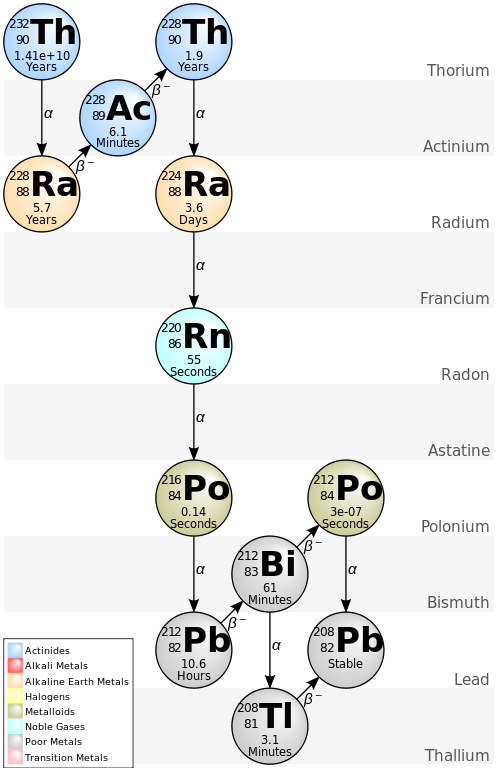
\includegraphics[width=.34\textwidth]{C:/Users/Niko/Documents/LaTex/Nick_K_Thesis/CH3_figs/Th232_chain.png}
\caption{One decay chain for Th-232, which ends with the stable isotope Pb-208. The long half-life of Th-232 allows one to assume a secular equilibrium for undisturbed samples with Th-232 contamination. The figure shows the half-lives of the isotopes, as well as their method of decay.}
\end{wrapfigure}

Secular equilibrium is the assumption of a near-equilibrium in the decay chain of a radioisotope. It assumes that the decay rates for all daughters in a given decay chain are equal. It is a crucial concept for the following sections, so will briefly be explained here.

The validity of assuming secular equilibrium comes from the length of the half-lives of parent isotopes under examination. The isotopes screened for in Gopher are all very stable radioisotopes, with half lives on par with the age of the universe. This is crucial, as it means that over a given period of time, the decay rates of the isotopes are nearly constant (because the total population of the parent isotope doesn't change noticeably over time periods which are small compared to its half-life). Consider the decay chain for Th-232, shown in Figure 3.2. As Th-232 decays, Ra-228 particles are created at a constant rate. The Ra-228 particles will subsequently decay into Ac-228 particles, at a rate determined by their half-life. The population of Ra-228 will increase until its decay rate is equal to the constant creation rate. This will occur for Ac-228, Th-228, and all other daughters in the decay chain, with final decay rates being set by the decay rate of the initial Th-232 parent. Therefore, secular equilibrium yields an expected abundance for each daughter isotope in the decay chain -- based on their relative half-lives -- as well as identical decay rates for all daughters in the chain.

The assumption of secular equilibrium can be invalidated if the half-lives of the parent isotopes are not sufficiently long, or through processes which remove or add isotope populations and break secular equilibrium, such as refining. However, the assumption of secular equilibrium is often very useful in the analysis of radioactive contaminants.


\subsection{Measuring Radioactivity}
To measure the radioactivity of thermal stand-off candidates, we sent them to an underground facility in Soudan, Minnesota. This facility possesses a high-purity germanium detector, called Gopher, which is used as a gamma ray counter. The samples are cleaned thoroughly to remove any contaminants then placed inside a low background environment with the detector, and allowed to remain until sufficient gamma counts are detected for analysis.

\begin{SCfigure}[.6][h]
\centering
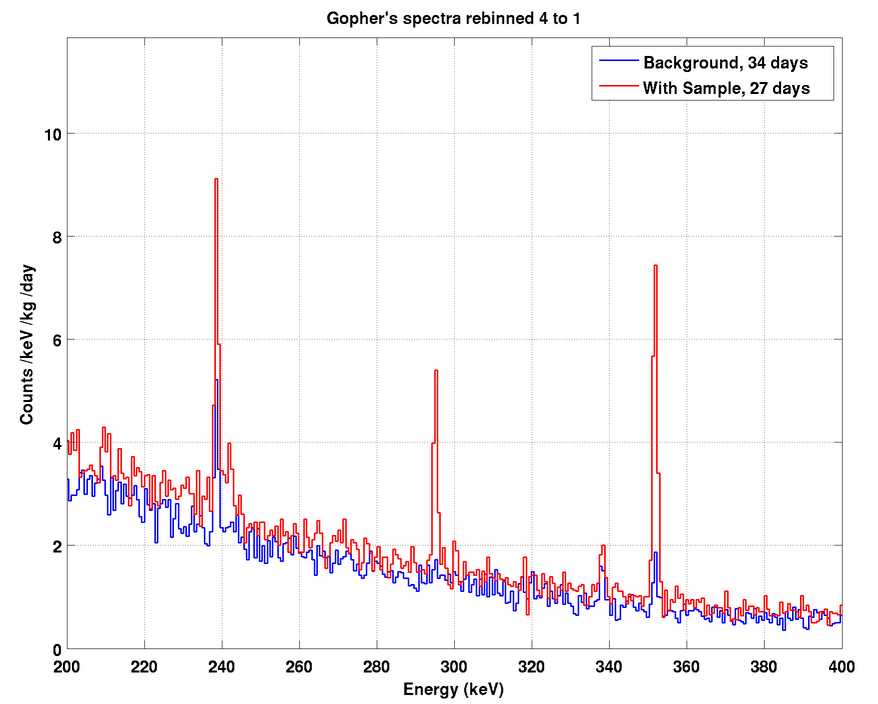
\includegraphics[width = .5\textwidth]{C:/Users/Niko/Documents/LaTex/Nick_K_Thesis/CH3_figs/Gopher_counts_v_background.png}
\caption{Detected gamma spectrum from 200keV - 400keV for a counted Ti 15-3-3-3 foil as obtained from Gopher -- a high purity Ge detector in Soudan, Minnesota. Background counts are shown in blue, while the sample spectrum peaks are clearly visible in red above the background. The 295keV Pb-214 line, for example, is clearly visible in the middle of the plot. Plot from \cite{GopherTi15333}.}
\end{SCfigure}

\subsubsection{Counting}
The counting process itself relies on low backgrounds which are precisely characterized. Once a background spectrum is obtained, the sample is placed in the detection chamber and counted until a reliable activity above background is obtained. Figure 3.2 shows such a spectrum for a gamma energy of 200keV to 400keV, in which the sample activity (shown in red) is clearly visible above the background activity (in blue). Background is then subtracted away, and the count rate of prominent lines for isotopes of interest are determined. The long-lived isotopes currently screened for in Gopher are Th-232, U-238, Co-60, K-40, and Cs-137. An example of a prominent daughter isotope line -- the 295keV Pb-214 line from U-238 decay -- is shown in the center of Figure 3.2. Finding the gamma rate for specific daughter isotopes, however, is not enough to determine activity of the parent isotopes. Simulation is required for finding the total activity of the sample.

\subsubsection{GEANT4 Monte Carlo Simulation}
While radioactive screening with Gopher gives us the gamma emission rate for various radioisotopes, we are actually concerned with the decay rate of the isotopes in the sample (which is the rate of isotope disintegration into another isotope). To convert to true activity of the sample, the peak detection ratio must be determined for each line. This is accomplished by GEANT4 Monte Carlo simulation of the sample.

GEANT4 (GEometry ANd Tracking) is a set of scripts which, through Monte Carlo methods, simulates the passage of particles through matter. This simulation takes into account many factors such as the geometry of the sample, position with respect to the detector, gamma intensity for various decay methods, and composition of the sample to estimate the peak detection ratio, defined as [number of counts observed for a line]/[number of MC-simulated events for a line] which simply determines what fraction of total events are detected as gammas in the detector. The Monte Carlo is run for each isotope in a chain by homogenously distributing that isotope through the sample. From here, given the considerations above, the peak detection ratio of detections/events for each isotope can be determined. Figure 3.3 shows a visualization of this process for Vespel SCP-5050. The right two figures show simulations of particle decay which track the movement/scattering of particles from the top and side perspective, respectively, while the leftmost figure shows the sample (dark rods) in the screening chamber with the Ge detector (silver cylinder in back).

\begin{figure}[h]
\centering
\begin{minipage}{.34\textwidth}
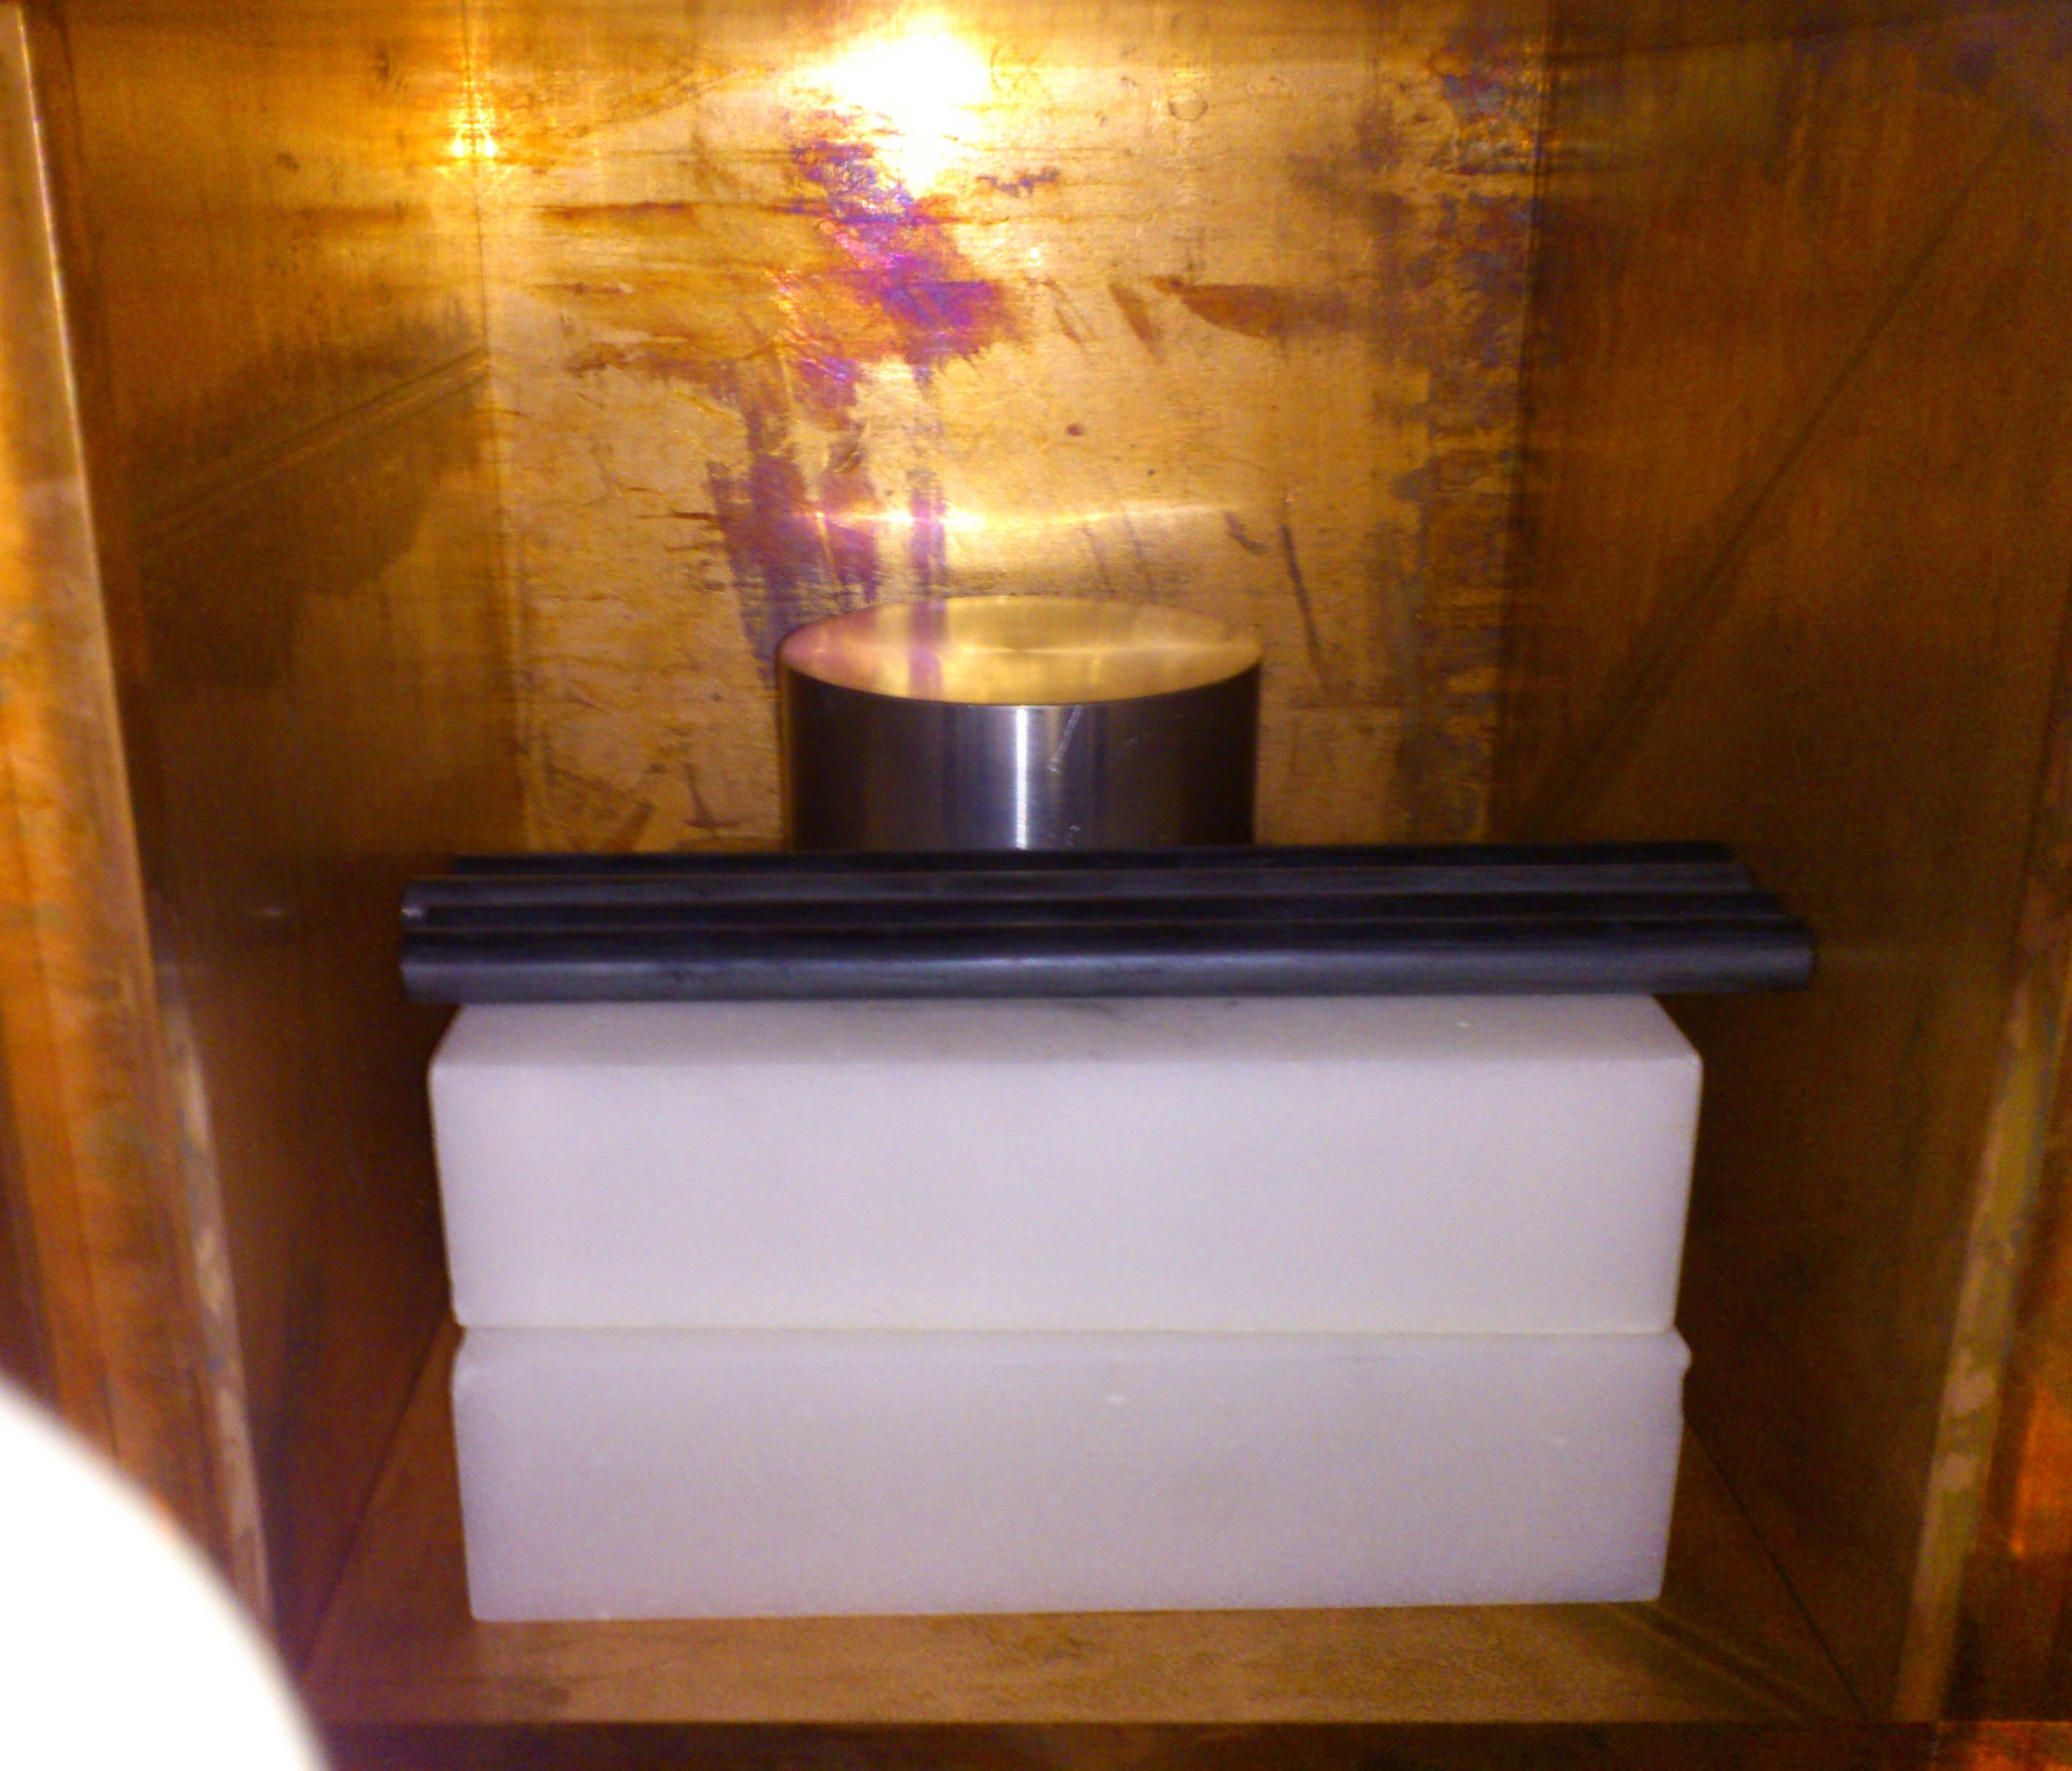
\includegraphics[width = \textwidth]{C:/Users/Niko/Documents/LaTex/Nick_K_Thesis/CH3_figs/VespelSCP5050_In_Gopher.jpg}
\end{minipage}
\begin{minipage}{.3\textwidth}
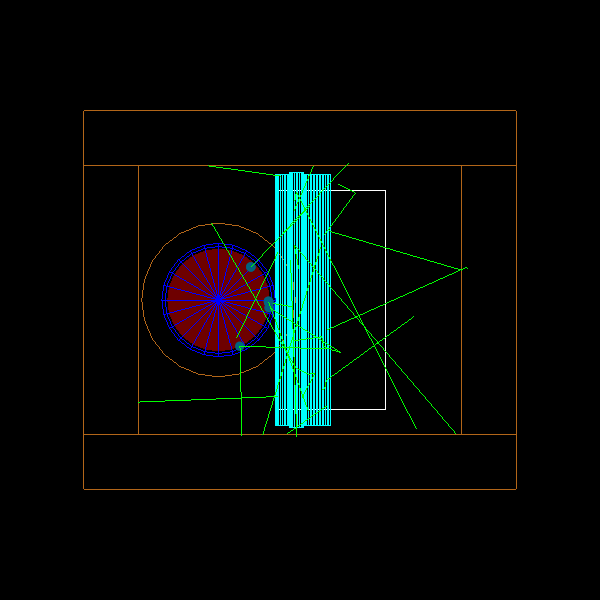
\includegraphics[width = \textwidth]{C:/Users/Niko/Documents/LaTex/Nick_K_Thesis/CH3_figs/VespelSCP5050_Top_Hits.png}
\end{minipage}
\begin{minipage}{.3\textwidth}
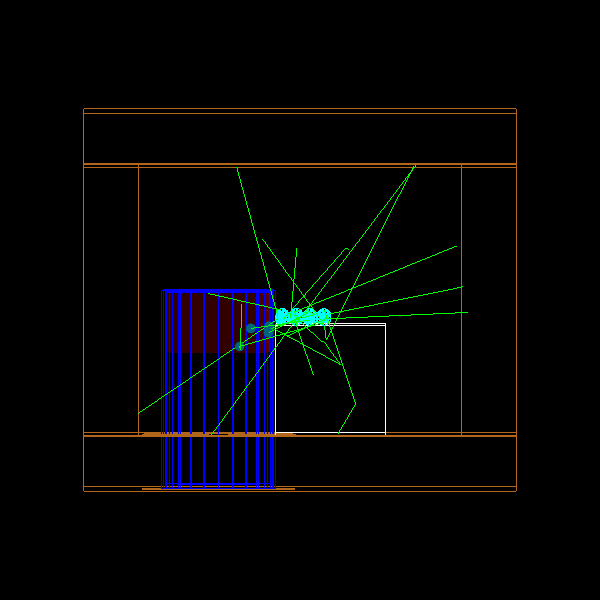
\includegraphics[width = \textwidth]{C:/Users/Niko/Documents/LaTex/Nick_K_Thesis/CH3_figs/VespelSCP5050_Side_Hits.png}
\end{minipage}
\caption{Vespel SCP-5050 sample in Gopher. The left figure shows the sample placement in the detection chamber, with PE. The middle and right figure show the GEANT4-MC simulations from the top and side perspectives, which track particle movement through the sample, chamber, and detector. Images from \cite{GopherSCP5050}.}
\end{figure}

\subsubsection{Determining Total Activity for Each Line}

Once the peak detection ratio is calculated for each line, the gamma rates can be converted to contamination. Then, assuming secular equilibrium, we know that the contamination (decays/second) should be equal for each isotope in a given decay chain. Due to the finite accuracy of statistics, this may not always be true, so a weighted average of the prominent daughter isotope contaminations is performed, which then gives the total contamination of the five parent isotopes screened for. Figure 3.5 shows the calculated contamination for various daughter isotopes of Th-232, U-238, Cs-137, Co-60, and K-40. These are the daughter contaminations that were used in Vespel SCP-5050 to determine parent isotope contamination.

\begin{SCfigure}[.5][h]
\centering
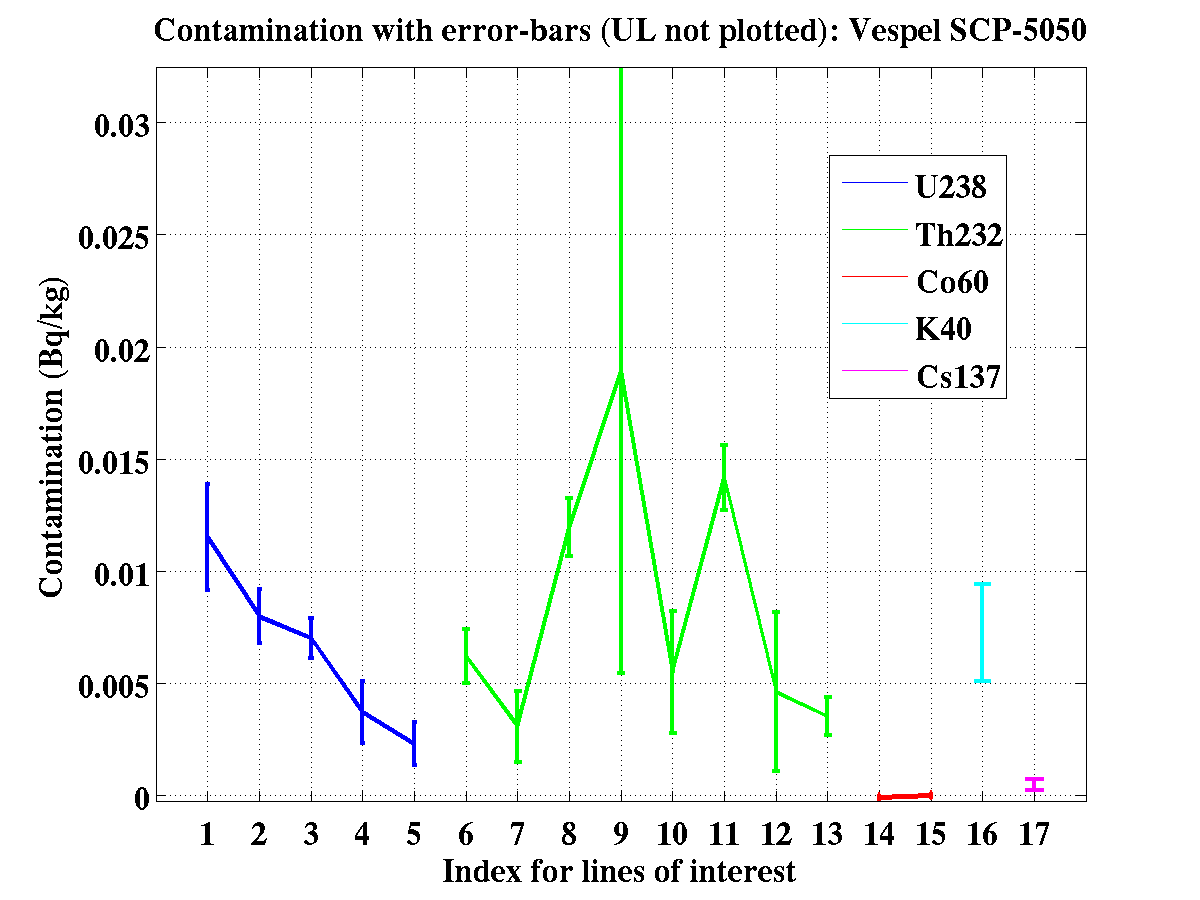
\includegraphics[width = .55\textwidth]{C:/Users/Niko/Documents/LaTex/Nick_K_Thesis/CH3_figs/SCP5050_contamination.png}
\caption{Calculated contamination of daughter isotopes used to determine contamination of each parent isotope. The indices represent specific lines for daughter isotopes in decay chains. 1-5 are for daughters of U-238, 6-13 are for daughters of Th-232, 14-15 are for Co-60, 16 is for K-40, and 17 is for Cs-137. Figure from \cite{GopherSCP5050}. }
\end{SCfigure}

\subsubsection{Results}

The results of Gopher screenings are shown in Figure 3.2 with contamination levels for different isotopes given in milliBecquerels/kilogram. The graphite currently in use, UF-4S (old), shows almost no contamination with $<2$ mBq/kg of U-238. However, new samples of the same material show much higher contamination levels, $\sim 50$mBq/kg of Th-232, despite purification. This irreproducibility in radiopurity levels between graphite batches has been a problem before; when originally purchased, one batch of UF-4S showed too much contamination to use. 2020 graphite is from the same company as UF-4S (Mersen) and shows similar levels of contamination as the new UF-4S stock. These levels are likely higher than what our experiment can tolerate. The next three graphite grades are from Poco Graphite: ACF-10Q, AXM-5Q, and ZXF-5Q. They are all industrial graphite grades, as compared with UF-4S and 2020, which are nuclear grade. This is apparent in their significantly higher contamination levels. The next counted sample, AXM-5Q (p) was purified by Mersen, in the process described below. This purification proved to be extremely effective, decreasing activity by a factor of $\sim50$ to acceptable levels. Vespel SP-1 shows low levels of contamination as well, making it an ideal candidate from a radioactivity level perspective. The next sample, Vespel SP-22 shows very high levels of contamination, due its high graphite content, which rule it out as a candidate for the thermal stand-offs. Surprisingly, SP-22's successor, Vespel SCP-5050, shows very promising levels of contamination, which may be acceptable depending on the amount used in the experiment. The next two samples, Ti 15-3-3-3 and Graphlite CFRP, show similar levels of contamination which again, may be acceptable depending on the mass used in the experiment.

\subsubsection{Graphite Purification}
Graphite such as AXM-5Q are of interest in our experiment, and in many experiments, due to their very low thermal conductivity. However, as the results of screening show, they are often contaminated with high levels (by our standards) of radioisotopes. Therefore, the purification processes offered by Mersen and Poco are of great interest. The results are clearly visible in Table 3.2 for AXM-5Q, which saw its activity reduced by a factor of 50 post-purification.

The purification process offered by Mersen reduced impurities from around 1000ppm to $<$1.4ppm for all purified samples (including those from Poco, which were sent to Mersen for purification) \cite{Mersen_conv}. The graphites are placed in an environment of chlorine gas pressurized above 15psi and heated to roughly $2000^{o}C$. In these conditions, the chlorine permeates the material and readily bonds with oxidizable metals to remove them from the sample \cite{Olivier_conv}. This is more effective the thinner/more porous the graphite.

\begin{table}[htb]
\centering
\begin{threeparttable}
\rowcolors{3}{gray!20}{white}
\begin{tabular}{l|rrrrr}
\multirow{2}{*}{\large{Material}} & \multicolumn{5}{c}{Contamination in mBq/kg}\\
& U-238 & Th-232 & Co-60 & K-40 & Cs-137 \\\toprule
UF-4S Graphite (old) & 1.33 $\pm$ 2.18 & - & - & - & -\\
UF-4S Graphite (new, p) & - & 52.03 $\pm$ 3.11 &- & -& - \\
2020 Graphite (p) & 3.89 $\pm$ 0.60 & 79.63 $\pm$ 2.02 &- & 4.10 $\pm$ 1.65 &- \\
ZXF-5Q Graphite (u-p) & 159.73 $\pm$ 4.37 & 218.11 $\pm$ 5.26 & - & - & - \\
ACF-10Q Graphite (u-p) & 406.77 $\pm$ 6.51 & 286.65 $\pm$ 5.73 & -& 35.90 $\pm$ 8.02 &-\\
AXM-5Q Graphite (u-p) & 117.71 $\pm$ 2.39 & 217.13 $\pm$ 3.79 &- & -&-  \\
AXM-5Q Graphite (p) & 0.93 $\pm$ 0.25 & 4.93 $\pm$ 0.70 & -& 0.96 $\pm$ 1.16 & - \\
Vespel SP-1 & -& 5.39 $\pm$ 4.80 & -& -&-  \\
Vespel SP-22 & 48.38 $\pm$ 4.83 & 211.10 $\pm$ 8.99 &- & 7.82 $\pm$ 6.09 &\\
Vespel SCP-5050 & 7.72 $\pm$ 0.69 & 9.95 $\pm$ 0.72 &- & 7.26 $\pm$ 2.18 & 0.48 $\pm$ 0.26 \\
TiMet$^{\circledR}$ Ti 15-3-3-3 & -& 17.20 $\pm$ 3.20 &- &- & - \\
Graphlite$^{\circledR}$ CFRP & 2.79 $\pm$ 0.89 & 0.707 $\pm$ 1.39 &- & 24.00 $\pm$ 4.96 & -\\

\end{tabular}
\caption{Activity of listed parent for each sample. Screened at Gopher, a high purity Ge
gamma counter in Soudan, MN. The two results for UF-4S graphite are from the old stock (currently in use in SuperCDMS Soudan) and new stock, purchased recently. For the graphites, u-p refers to unpurified stock samples, while p refers to those samples which have been purified by the method described in this section.}
\end{threeparttable}
\end{table}

\begin{table}[htb]
\centering
\begin{threeparttable}
\rowcolors{3}{gray!20}{white}
\begin{tabular}{l|ccccc}
\multirow{2}{*}{\large{Material}} & \multicolumn{3}{c}{$\frac{Neutrons}{year \cdot cm^{3}}$}\\
& Sponteneous Fission & ($\alpha$,n)-reactions & Total \\\toprule
CDMS Graphite & 2.1 $\cdot 10^{-4}$ & - & 2.1 $\cdot 10^{-4}$ \\
ZXF-5Q Graphite & - & - & - \\
ACF-10Q Graphite & - & - & - \\
AXM-5Q Graphite & - & - & - \\
Vespel SP-22 & - & - & - \\
Vespel SP-1 & - & - & - \\
Ti 15-3-3-3 & 3.04 $\cdot 10^{-7}$ & 2.09 $\cdot 10^{-6}$ & 2.4 $\cdot 10^{-6}$ \\

\end{tabular}
\caption{Neutron production per year for 1 $cm^{3}$ of material for candidate materials}
\end{threeparttable}
\end{table}

\subsection{Using SOURCES-4C to Predict Neutron Emission Rates}
Neutron background is the largest concern for our detectors as it produces a
nuclear recoil which, along with no charge collection, mimics the expected signal
from WIMPS. In our candidate materials, there are two sources of neutrons:
Spontaneous Fission and ($\alpha$,n)-reactions. The rates at which these occur for each material are determined by two factors: which radioisotopes are present in the material (determined by the Gopher screenings), and the elemental composition of the material. The elements in a material serve as the target materials for the ($\alpha$,n)-reactions, particularly low-Z elements (which have lower Coulomb barriers preventing the $\alpha$-particle from reacting with the nucleus). Therefore, the total activity for each material is not the primary determining factor; in an ideal situation, we would consider candidates based on acceptable neutron emission rates.

To model the neutron emission rate of each material, we used SOURCES-4C, a program
developed by Los Alamos National Laboratory and Texas A\&M University. This
program allows calculation of neutron emission rates through both spontaneous
fission and ($\alpha$,n)-reactions using an extensive library of parameters
such as reaction and stopping cross-sections,product nuclide level branching
fractions, etc.

For our problem, the input parameters for SOURCES-4C were:
\begin{enumerate}
\item Constituent elements in atom fraction
\item Alpha sources in atoms/cc
\item Target materials in atom fraction
\end{enumerate}

To determine the $\alpha$-source contamination in atoms/cc we have to convert
from the total activity values in Table 3.2. To do this, we first find the concentration of the parent isotopes given in the table. This is done by starting with the equation for the time-dependent population of a radioisotope,
\begin{eqnarray}
D(t) & =& D_0\left(\frac{1}{2}\right)^{t/h} \\
\end{eqnarray}
where D(t) is the population at any time t, $D_0$ is the population at t = 0, and h is the half-life of the particle in seconds. Taking the derivative of both sides, we can find the rate of change in population at any t. This gives
\begin{eqnarray}
D'(t) = \frac{ln\left(\frac{1}{2}\right)}{h}D_0\left(\frac{1}{2}\right)^{t/h} = \frac{ln\left(\frac{1}{2}\right)}{h}D_0 \ \ , \ \ t << h \\
\end{eqnarray}

the simplification on the right side of the equation comes from observing that t is always small when compared to the half-lives of the parent isotopes under consideration, so $(1/2)^{t/h} \sim 1$. To get to atoms/$cm^3$ we convert D'(t) to R (activity in Bq/kg), multiply by material density, $\rho$ (in $kg/cm^3$), and rearrange:

\begin{eqnarray}
D_0 = D = -\frac{R \rho h}{ln\left(\frac{1}{2}\right)}
\end{eqnarray}

where the R for each parent isotope comes from the screening results.

Once we have the contamination of the parent isotope we can then find the
corresponding contamination for all $\alpha$-emitting daughters by assuming secular equilibrium. This allows us to set R equal for all isotopes in a decay chain. Exploiting this equality in 3.6, we obtain
\begin{eqnarray}
\frac{D_i}{h_i} = \frac{D_k}{h_k}
\end{eqnarray}
where the subscripts denote different isotopes in secular equilibrium. This says that, in secular equilibrium, the ratio of isotopes present in a given decay chain depends only on the ratio of those isotopes' half-lives. This can be applied to find the amount of each daughter isotope from the parent isotope in a chain with,
\begin{eqnarray}
D_{d} = D_{p}\frac{h_{d}}{h_{p}}
\end{eqnarray}

where the subscripts d and p refer to daughter and parent, respectively.



\section{Thermo-Mechanical Properties}

The tower thermal stand-offs are a structural component of the tower, so the physical and mechanical properties of the materials are naturally an important factor in choosing suitable candidates. In Table 3.4 \& 3.5 I examine some of the physical quantities of interest for possible thermal stand-offs materials. These numbers characterize the strength and dimensional stability of the materials. Dimensional stability is required to ensure the correct operation of our rigid vacuum coaxes; if the tower flexes too much during handling, the vacuum coaxes could be put under too much tension and snap. Similarly, during fridge operation, a CTE which is too high could cause the vacuum coaxes too go slack and short to their shielding; a CTE which is too low could cause too much tension and plastically deform the lines. The different strength parameters are crucial in telling us how little of the material we can safely use in creating a sufficiently strong support. Since radioactivity levels and thermal power conducted depend on volume and cross-section of the material, respectively, by minimizing material use we also minimize radioactivity and thermal loads to the dilution fridge stages.

\begin{table}[htb]%THERMOPHYSICAL PROPERTIES
\begin{threeparttable}
\rowcolors{3}{gray!20}{white}
\begin{tabular}{lcccccc}
\toprule
\textbf{Material} & $\rho$ ($g/cm^3$) & $\nu$ & $\sigma_{t}$ (MPa) & $\sigma_{c}$ (MPa)
& $\sigma_{f}$ (MPa) & CTE $(\mu m/(m\cdot C^o))$ \\
\midrule
 UF-4S Graphite & 1.76  & 0.2 & 20$^{\dag}$ & 50$^{\dag}$ & 27.6 & 1.8-2.9 \\
 2020 Graphite & 1.77 & 0.15 & 29 & 98 & 45 & 4.3 \\
 POCO AXM-5Q & 1.73 & 0.3$^{*}$ & 48 & 124 & 69 & 7.8 \\
 Ti 15-3-3-3 & 4.71 & 0.36 & 1117 & 1052 & - & 8.45 \\
 Ti 21S & 4.93 & 0.34 & 958 & 1108 & - & 7.07 \\
 Vespel SP-1 & 1.43 & 0.41 & 86.2 & 133 & 110 & 54.0$^{\ddag}$ \\
 Vespel SCP-5000 & 1.46 & - & 163 & 640 & 254 & 45.0 \\
 Vespel SP-22 & 1.65 & - & 51.7 & 112 & 89.6 & 38.0 \\
 Vespel SCP-5050 & 1.76 & 0.22 & 72 & 219 & 130 & 29.0 \\
 Graphlite CF Rod & 1.55 & -  & 2340 & 1900 & - & - \\
 \bottomrule
\end{tabular}
\caption{Some thermo-mechanical properties of candidate materials. $\nu$ is the Poisson's ratio for the material, while $\sigma_{t}$,$\sigma_{c}$, and $\sigma_{f}$ are tensile, compressive, and flexural strengths for the material, respectively. CTE is the linear coefficient of thermal expansion, given at room temperature for all materials. The properties given for Ti 15-3-3-3 and Ti 21s are lower limits for solution-treated, age-hardened samples. These numbers can be higher or lower depending on the specific heat treatment. All Vespel data are for Isostatically-formed parts. All Graphlite CFRP data is along the fiber axis. \dag - Compressive and tensile strengths were derived from the flexural strength, using an apparent trend in graphite materials where tensile $\approx$ 2/3 flexural and compressive $\approx$ twice flexural. * - A poisson ratio of 0.3 is typical for many graphites. \ddag - DuPont data for SP-1 gives a CTE of 45 $(\mu m/(m\cdot C^o))$ for -62$^{o}$C - 23$^{o}$C, whereas the number given in the table is for 23$^{o}$C and above. for Ti 15-3-3-3 and Ti 21s from \cite{Nyakana2005} and \cite{Johnson1996}. All other data from manufacturer websites or datasheets.}
\end{threeparttable}
\end{table}

\begin{table}[htb]
\begin{threeparttable}
\rowcolors{3}{gray!20}{white}
\begin{tabular}{lccc}
\toprule
\textbf{Material} & $E_{T}$ (GPa) & $E_{C}$ (GPa) & G (GPa) \\
\midrule
 UF-4S Graphite & 7.2 & - & 3$^{\ddag}$ \\
 2020 Graphite & 9.2 & - & 4.1 \\
 POCO AXM-5Q & 10.5 & - & 4$^{\ddag}$ \\
 Ti 15-3-3-3 & 105 & - & 39.5$^{\ddag}$ \\
 Ti 21S & 103 & 114 & 38.7$^{\ddag}$ \\
 Vespel SP-1 & - & 2.41 & - \\
 Vespel SCP-5000 & 3.99 & 9.06 & 1.41$^{\ddag}$\\
 Vespel SP-22 & - & 3.28 & - \\
 Vespel SCP-5050 & 8.93 & 3.00 & 3.66$^{\ddag}$\\
 Graphlite CF Rod & 134 & 131 & - \\
 \bottomrule
\end{tabular}
\caption{Continuation of table 3.4 for thermo-mechanical properties. Different moduli are given for each material: $E_{T}$ is the Young's Modulus, $E_{C}$ is the compressive modulus, and G is the shear modulus. \ddag - Indicates that data on the shear modulus, G, was unavailable; instead, the formula for homogenous and isotropic materials was used, in which $G = E_{T}/(2(1 + \nu))$. References are the same as above. }
\end{threeparttable}
\end{table}

One of the most noticeable aspects of Tables 3.4 \& 3.5 is the wide distribution of structural properties for materials. As with any other qualification discussed in this chapter, some candidates are clearly better suited mechanically; however, this simply reflects the wide array of parameters which must be satisfied, and that different materials were chosen for different particular merits. Below I summarize the interesting results from the tables:
\begin{itemize}
\item UF-4S Graphite (used as a thermal stand-off in SuperCDMS Soudan) has lower strengths than every other material including AXM-5Q,
another graphite. It also has the lowest CTE, which made it well suited as a thermal stand-off in the current towers, where small stage separations demanded minimal contractions to prevent thermal shorts between stages.
\item The two Ti alloys from TiMetal, Ti15-3-3-3 and Ti21s, offer some of the highest strengths of the candidates coupled with low CTEs and high elastic moduli, making them strong candidates.
\item The Vespel SCP series compounds outperform their SP counterparts in nearly every regard. Their strengths show an increase of between 50\% - 400\%, with increased elastic moduli, and decreased coefficients of thermal contraction.
\item Vespel SCP-5000 still has a fairly high CTE -- 45 ppm/C at room temperature. The number below room temperature is likely lower, however, if SCP-5000 follows the same trend as SP-1; this trend gives a CTE for SP-1 of 54ppm/C at room temperature and above, which drops to 45ppm/C from -62$^{o}$C - 23$^{o}$C.
\item Graphlite CFRP offers exceptionally high strength as well as dimensional stability, which suggests that we could safely use very little of the material in order to minimize radioactivity and heat loads.
\end{itemize}

From here, we can now develop models which examine the interplay of properties for these materials.


\section{Thermal Contraction}

The thermal contraction of our tower stand-offs is constrained by the rigid vacuum NbTi coaxes, as described in chapter 2. We must ensure that these coaxes do not experience excessive strain and that they do not go slack during cooldown, which could short them to their copper housing. This is the only constraint, as the new SNOLab tower will feature an open face design, eliminating the 0.03" copper-copper stage separation, along with the need to preserve such a small separation during cooldown.

\begin{figure}[ht]
\centering
\subfloat[Simplified SNOLab tower used to calculate expected thermal contraction behavior of tower components. All stand-off lengths and NbTi coax lengths are assumed to be 2", making the analysis identical for all tower stages.]{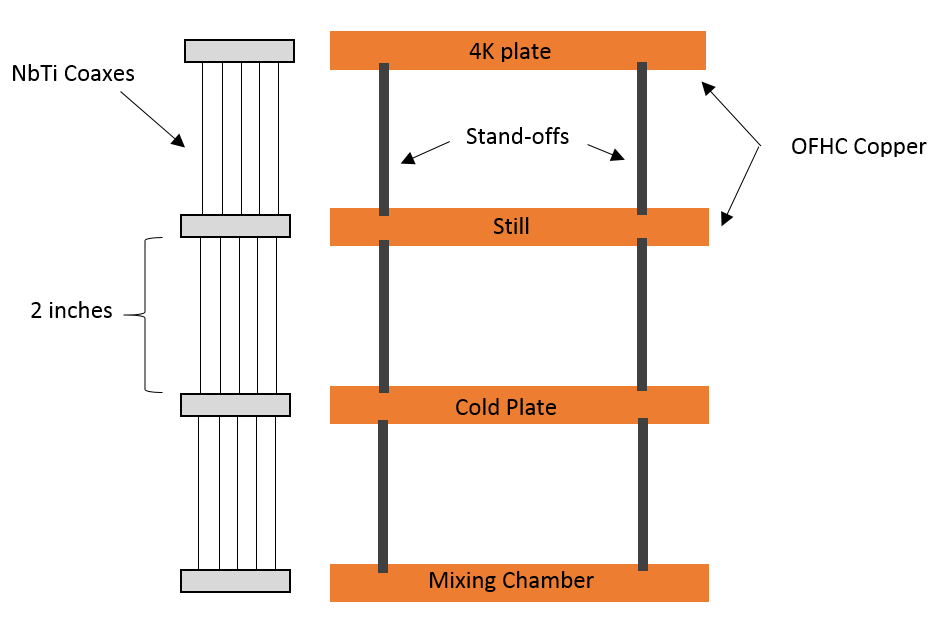
\includegraphics[width = .5\textwidth]{C:/Users/Niko/Documents/LaTex/Nick_K_Thesis/CH3_figs/SNOLab_tower_coax_stress.png}}
\qquad
\subfloat[Model for deflection of NbTi coaxes, where any slack is efficiently translated into a deflection. L is the distance between the coax heat-sinks, and $L_eq$ is the equilibrium length of the NbTi wires at 4K. A deflection $\geq$ 0.021" means that the wires will short to their housing]{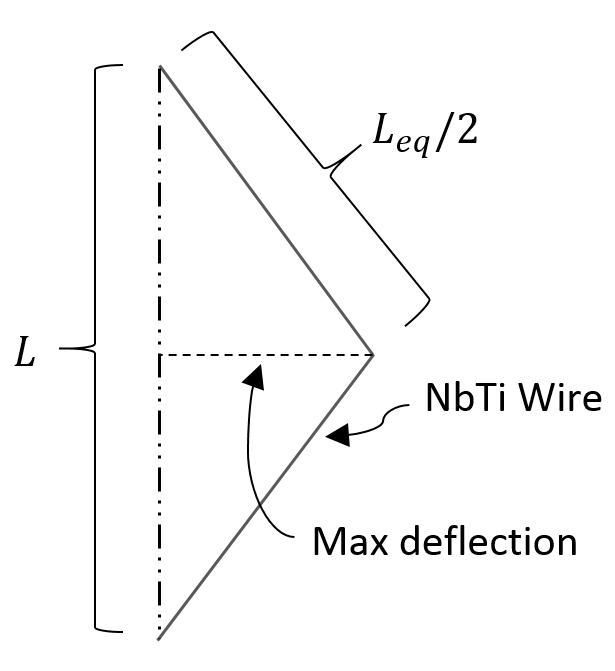
\includegraphics[width = .33\textwidth]{C:/Users/Niko/Documents/LaTex/Nick_K_Thesis/CH3_figs/NbTi_deflection.png}}
\caption{SNOLab model used to determine the strain in the NbTi wires (a), and the slack formed (b) during cooldown.}
\end{figure}

The model used for the SNOLab towers, shown in Figure 3.6a, is simple: it assumes stand-off lengths and vacuum coax lengths are all 2", and considers only the NbTi and stand-off contraction, without considering the CFRP support struts for the coaxes. Much of the analysis follows a previous analysis performed for the Soudan towers, which can be read in greater detail in Appendix A.

\subsection{Strain}
Our goal is to find the strain on the vacuum coax wires during operation of our fridge. This strain can be positive or negative, where a negative strain represents the wires going slack. To find the strain, we use the formula
\begin{eqnarray}
Strain = \frac{L - L_{eq}}{L_{eq}}
\end{eqnarray}
where $L$ is the length of the wires at operating temperature, while $L_{eq}$ is the equilibrium length of the wires at that same temperature (under no strain). In our simple model, L is given at 4K by
\begin{eqnarray}
L = L_{NbTi} - |\Delta L_{stand-off}|
\end{eqnarray}
where $L_{NbTi}$ is the length of the wires at 300K, and $\Delta L_{stand-off}$ is the contraction of the stand-off from 300K to 4K \footnotemark. At the same time, $L_{eq}$ is given by
\begin{eqnarray}
L_{eq \ 300K} & = & L_{NbTi} \cdot (1 - 0.0107) \\
L_{eq} & = & (L_{eq \ 300K})\cdot\left(1 - \left|\frac{\Delta L_{NbTi}}{L_{NbTi}}\right|\right)
\end{eqnarray}
where $L_{NbTi}$ is the actual length of the NbTi wires at 300K, $L_{eq \ 300K}$ and $L_{eq}$ are the equilibrium lengths at 300K and 4K respectively, $\Delta L_{NbTi}/L_{NbTi}$ is the fractional contraction of the wires from 300K to 4K, and the 0.0107 term accounts for the fact that the wires are strained to 1.07\% during fabrication. The fractional contraction of the NbTi wires was calculated from A.1, while the total contraction of various stand-off materials is given by
\begin{eqnarray}
\Delta L = (CTE)(L_{stand-off})(\Delta T)
\end{eqnarray}
where $\Delta L$ is the length change of the stand-off, CTE is the coefficient of thermal contraction -- given by Table 3.4 for various materials, $L_{stand-off}$ is the 300K length of the stand-off, and $\Delta T$ is the total temperature change of the stand-off.

\footnotetext{The thermal contraction formula for NbTi only extended down to 4K. Since the contraction from 4K to $<$1K is negligible compared to the contraction from 300K to 4K, it was ignored.}

The above method was applied to our simple model, producing the upper plot in Figure 3.7. This gives the strain in the NbTi wires at 4K as a function of CTE for stand-off materials. We see that on the lower end, the strain doesn't exceed 1.2\% -- only slightly higher than fabrication strain, and within acceptable limits, according to Figure A.3. On the upper end, the wires experience a "negative strain", which means they have gone slack. This is investigated below

\begin{figure}[ht]
\centering
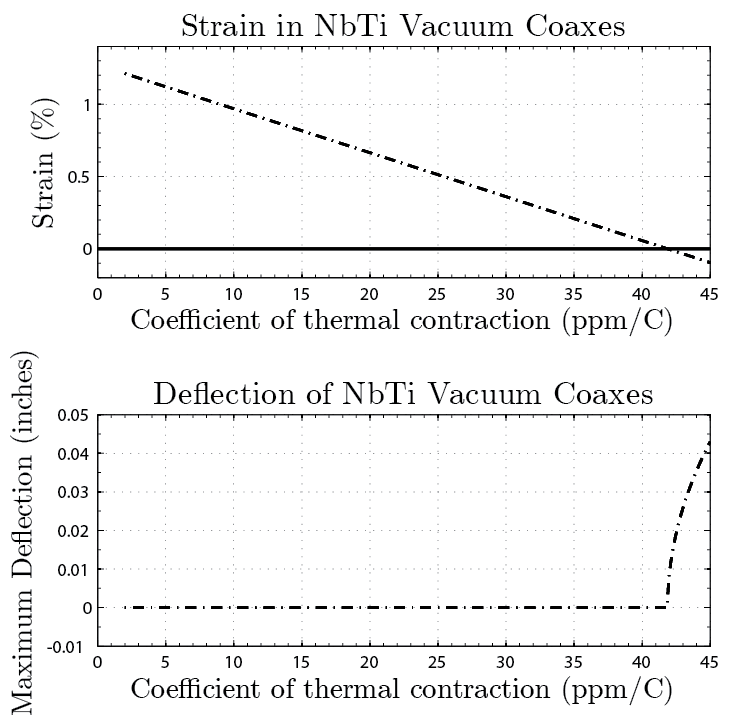
\includegraphics[width = .6\textwidth]{C:/Users/Niko/Documents/LaTex/Nick_K_Thesis/CH3_figs/Coax_strain.png}
\caption{}
\end{figure}

\subsection{Determining Slack in Wires}

The NbTi wires in our vacuum coax lines are suspended and centered in copper grooves which act as shielding during operation. Any slack in the wires could result in a short to these copper grooves, therefore we must determine if the slack experienced by the wires for various stand-off materials may cause a short.

The copper grooves surrounding the wires are 0.042" wide, which means that a deflection of 0.021" in either direction will cause a short to the housing. The model used to test this is shown in Figure 3.6b. We assume that any slack in the wire is perfectly taken up as a deflection (as if one was pulling the wire to the side). The calculated deflection, using this model, is shown in the lower plot of Figure 3.7 as a function of linear coefficients of thermal contraction for tower stand-off materials.

We see that there is no deflection in the wires until the linear CTE of the stand-off reaches 42ppm/C, which is the point when the strain at 4K reaches 0\%. From here, deflection increases rapidly past the 0.021" maximum allowable. In Table 3.4 we see that Vespel SP-1 and Vespel SCP-5000 are above the 42ppm/C limit. As noted in Table 3.4, however, the CTE of these materials is likely lower than the room temperature value given. The CTE of Vespel SP-1 drops from 54ppm/C for room temperature and above, to 45ppm/C below room temperature. Since Vespel SCP-5000 is similar to SP-1, its room temperature CTE of 45ppm/C would likely drop sufficiently low below room temperature to allow its use as a stand-off. If SCP-5000 was chosen for use in the fridge, however, it would be prudent to verify its low temperature CTE.

\subsection{Candidates Based on Thermal Stability}
Considering the strains and deflections found in Figure 3.7 for the range of CTE's found in our candidates, we conclude that all materials besides Vespel SP-1 should satisfy thermal stability requirements in the SNOLab towers, though the low temperature thermal contraction of Vespel SCP-5000 should be verified if it is chosen as a stand-off material.

\section{Tube Failure Model}

The dimensions of the SuperCDMS Soudan thermal stand-offs were selected arbitrarily, based on what sounded reasonable at the time; therefore, we are not attached to these dimensions. Ideally, the dimensions would be different for each material, designed in such a way as to take advantage of the strengths of each. This dimension optimization would allow us to minimize the use of material, reducing both thermal concerns and radioactivity concerns. This section presents a model developed in collaboration with professor Sanjay Govindjee of UC Berkeley, which considers four failure modes: shear buckling, bending buckling, normal material failure, and shear material failure. Using this model, we determine how little material can safely be used to withstand a 145lb. transverse shear load. We then compare the resulting heat loads and radioactivity for candidates given their optimized dimensions.

\subsection{Loading Conditions}

\begin{figure}[ht]
\centering
\subfloat[]{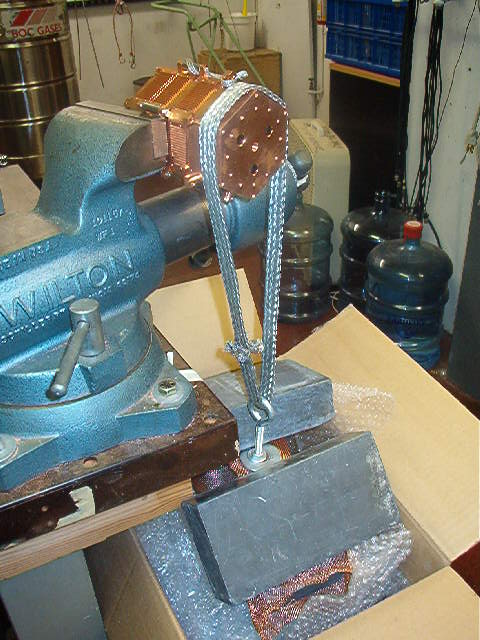
\includegraphics[width = .3\textwidth]{C:/Users/Niko/Documents/LaTex/Nick_K_Thesis/CH3_figs/Tower_loading.jpg}}
\qquad
\subfloat[]{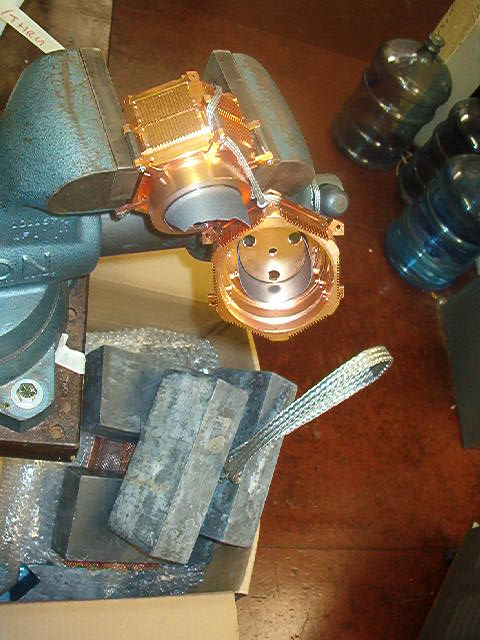
\includegraphics[width = .3\textwidth]{C:/Users/Niko/Documents/LaTex/Nick_K_Thesis/CH3_figs/Tower_break.jpg}}
\caption{Destructive physical analysis of Soudan tower. The 600mK floor was bolted to the 50mK tabs to support it, isolating the 10mK floor and its support. This was then loaded until failure under transverse shear. It failed at $\sim$145 pounds in what appears to be compressive failure.}
\end{figure}

The load conditions which we wish to design to for the SNOLab towers are not yet defined; therefore, as a first pass, we will consider it sufficient to replicate the strength of the Soudan tower stand-offs, which are able to withstand up almost 145lbs applied as a transverse shear force. This was found through a destructive physical analysis (DPA) of a Soudan tower. The tower was clamped in a bench vise, and the 600mK floor was bolted to the 50mK tabs to support it the 600mK to 50mK tube. This isolated the 10mK floor and the tube attached to it. A strap was hung over the 10mK floor, and loaded to $\sim$145 pounds before the tube failed. The load conditions and tube failure are shown in Figure 3.8. This load can be approximated by a transverse shear load. Therefore, our model will design stand-offs which can support 145 pounds as a transverse shear load.

\subsection{Analytical Model for Tube Failure}

Through discussion with Dr. Sanjay Govindjee at UC Berkeley, a model predicting failure loads for different materials/dimensions as well as optimization of Radius/Thickness (a/t) has been developed. The load considered is the same as that used in the Soudan tower DPA (one end fixed, the other subjected to a transverse shear force). This section develops this analytical model as well as its assumptions and limitations. Though an FEA model could be created (and will be to check the results), an analytical model is useful, as it lets one view the entire parameter space and failure trends. Given the prevalence of thin-walled tubes in cryogenic structures, this model has the potential to be of use in broader applications than our own.

Our model considers 4 failure modes:
\begin{itemize}
\item Shear Instability (Buckling)
\item Bending Instability (Buckling)
\item Material Failure from Normal Stresses
\item Material Failure from Shear Stresses
\end{itemize}

A discussion of the formulas for failure modes considered and their validities follow.

\subsubsection{Tube Geometry}
Cylindrical shell theories depend heavily on certain parameters in the shell, as these permit various simplifications of mechanical models. The graphite tube tested had nominal dimensions of thickness $t = 0.028$in, radius $a = 0.986$in (to middle surface), and length $L=1.334$in.

For theory, the relevant geometric ratios are
\begin{eqnarray}
\frac{a}{t} = 35.2 \\
\frac{L}{a} = 1.35 \\
Z = \frac{(1-\nu^2)^\frac{1}{2}L^2}{at} = 61.5 \ (\text{for $\nu$ = 0.3})
\end{eqnarray}

where Z is Donnell's parameter. These values imply a fairly thin shell of intermediate length. For dimension optimization, these values may change, and the model may need adjustment. Below are the formulas which are used for Z near this value.

\subsubsection{Shear Instability}

The tube may fail due to shear instability. According to Yamaki, this will occur when the maximum shear stress, $\tau_{f} = P/\pi at$ exceeds critical torsional stress from a purely torsional load,
$$
\tau{b} = \frac{\pi^2E}{12(1-\nu^2)}(1-\nu^2)^{\frac{3}{8}}a_s\left(\frac{t}{a}\right)^{\frac{5}{4}}\left(\frac{a}{L}\right)^{\frac{1}{2}}~~,
$$

where $a_{s}$ is between 0.81 and 1.04 for $Z \in [50,100]$. As dimensions change, Z could become as high as 400, for which $a_{s}$ is between 0.81 and 0.91. For either case, the lower value of 0.81 is taken to be conservative.

The number of circumferential waves present in buckling is
$$
N = \pi(1-\nu^2)^{\frac{1}{8}}b_{s}\left(\frac{a}{L}\right)^{1/2}\left(\frac{a}{t}\right)^{1/4},
$$
where $b_{s}$ is between 0.8 to 1.15 for the range of Z values.

This value gives between 3 and 5 waves depending on material/dimensions. Donnell's (typically used above 5 waves though!) shell theory will only give errors of $\sim$4\% at 3 waves. Above 3 waves the error decreases quickly. For graphite at current dimensions we have 5 waves, assuring accuracy.

To get critical load ($P_{c}$), set $\tau_{f} = \tau_{b}$ and solve for P:
$$
P_{c}^{s} = \frac{\pi^3E}{12(1-\nu^2)^{\frac{-5}{8}}}a_{s}\frac{a^{1/4}t^{9/4}}{L^{1/2}}
$$

\subsubsection{Bending Instability}

Bending instability can also occur in the case of transverse loading. This will occur as local buckling when the maximum stress (tensile or compressive) is exceeded. Approximating the tube as a membrane, the stress is $\sigma_{b} = PL/a^2t\pi$. The tube fails at a critical stress reasonably approximated by
$$
\sigma_{c}=\frac{E}{\sqrt{3(1-\nu^2)}}\frac{t}{a}.
$$

Combining these gives the critical load for localized bending buckling as:

$$
P_{c}^{b} = \frac{E \pi}{\sqrt{3(1-\nu^2)}}\frac{t^2a}{L}
$$
\subsubsection{Material Failure: Normal Stresses}

The material may fail simply from exceeding its normal stress limit, $\sigma_{f}$ where $\sigma_{f}$ is the minimum of tensile or compressive strength. Then the failure load for this failure is:
$$
P_{c}^{mb} = \sigma_{f} \pi \frac{a^2t}{L}
$$
\subsubsection{Material Failure: Shear Stresses}

Failure can also occur from the tube exceeding its shear stress limit, $\tau_{f}$. In ductile materials, $\tau_{f} \approx \sigma_{f}/2 \ \text{or} \ \sigma_{f}/\sqrt{3}$. Brittle material values (such as graphite) can be approximated from $\tau_{f} = \sigma_{t}\sqrt{R/3} $ where $R = \sigma_{c}/\sigma_{t}$ (compressive/tensile).

Given $\tau_{f}$, the predicted critical load for shear failure is:
$$
P_{c}^{ms} = \tau_{f}\pi at
$$

\subsubsection{Plotting Failure Curves}

Using the available material properties, we are able to produce the following graphs in figure 2. Each point along each line represents the radius and thickness that will give a failure load of 145lbs (as found in Dennis' tower break test). The upper right side of each line represents safe design dimensions. The green line follows the dominating failure mode at any point along the graph, therefore, the dimension space above this line represents safe design space.

%\begin{figure}[htb]
%\begin{minipage}[t]{.45\textwidth}
%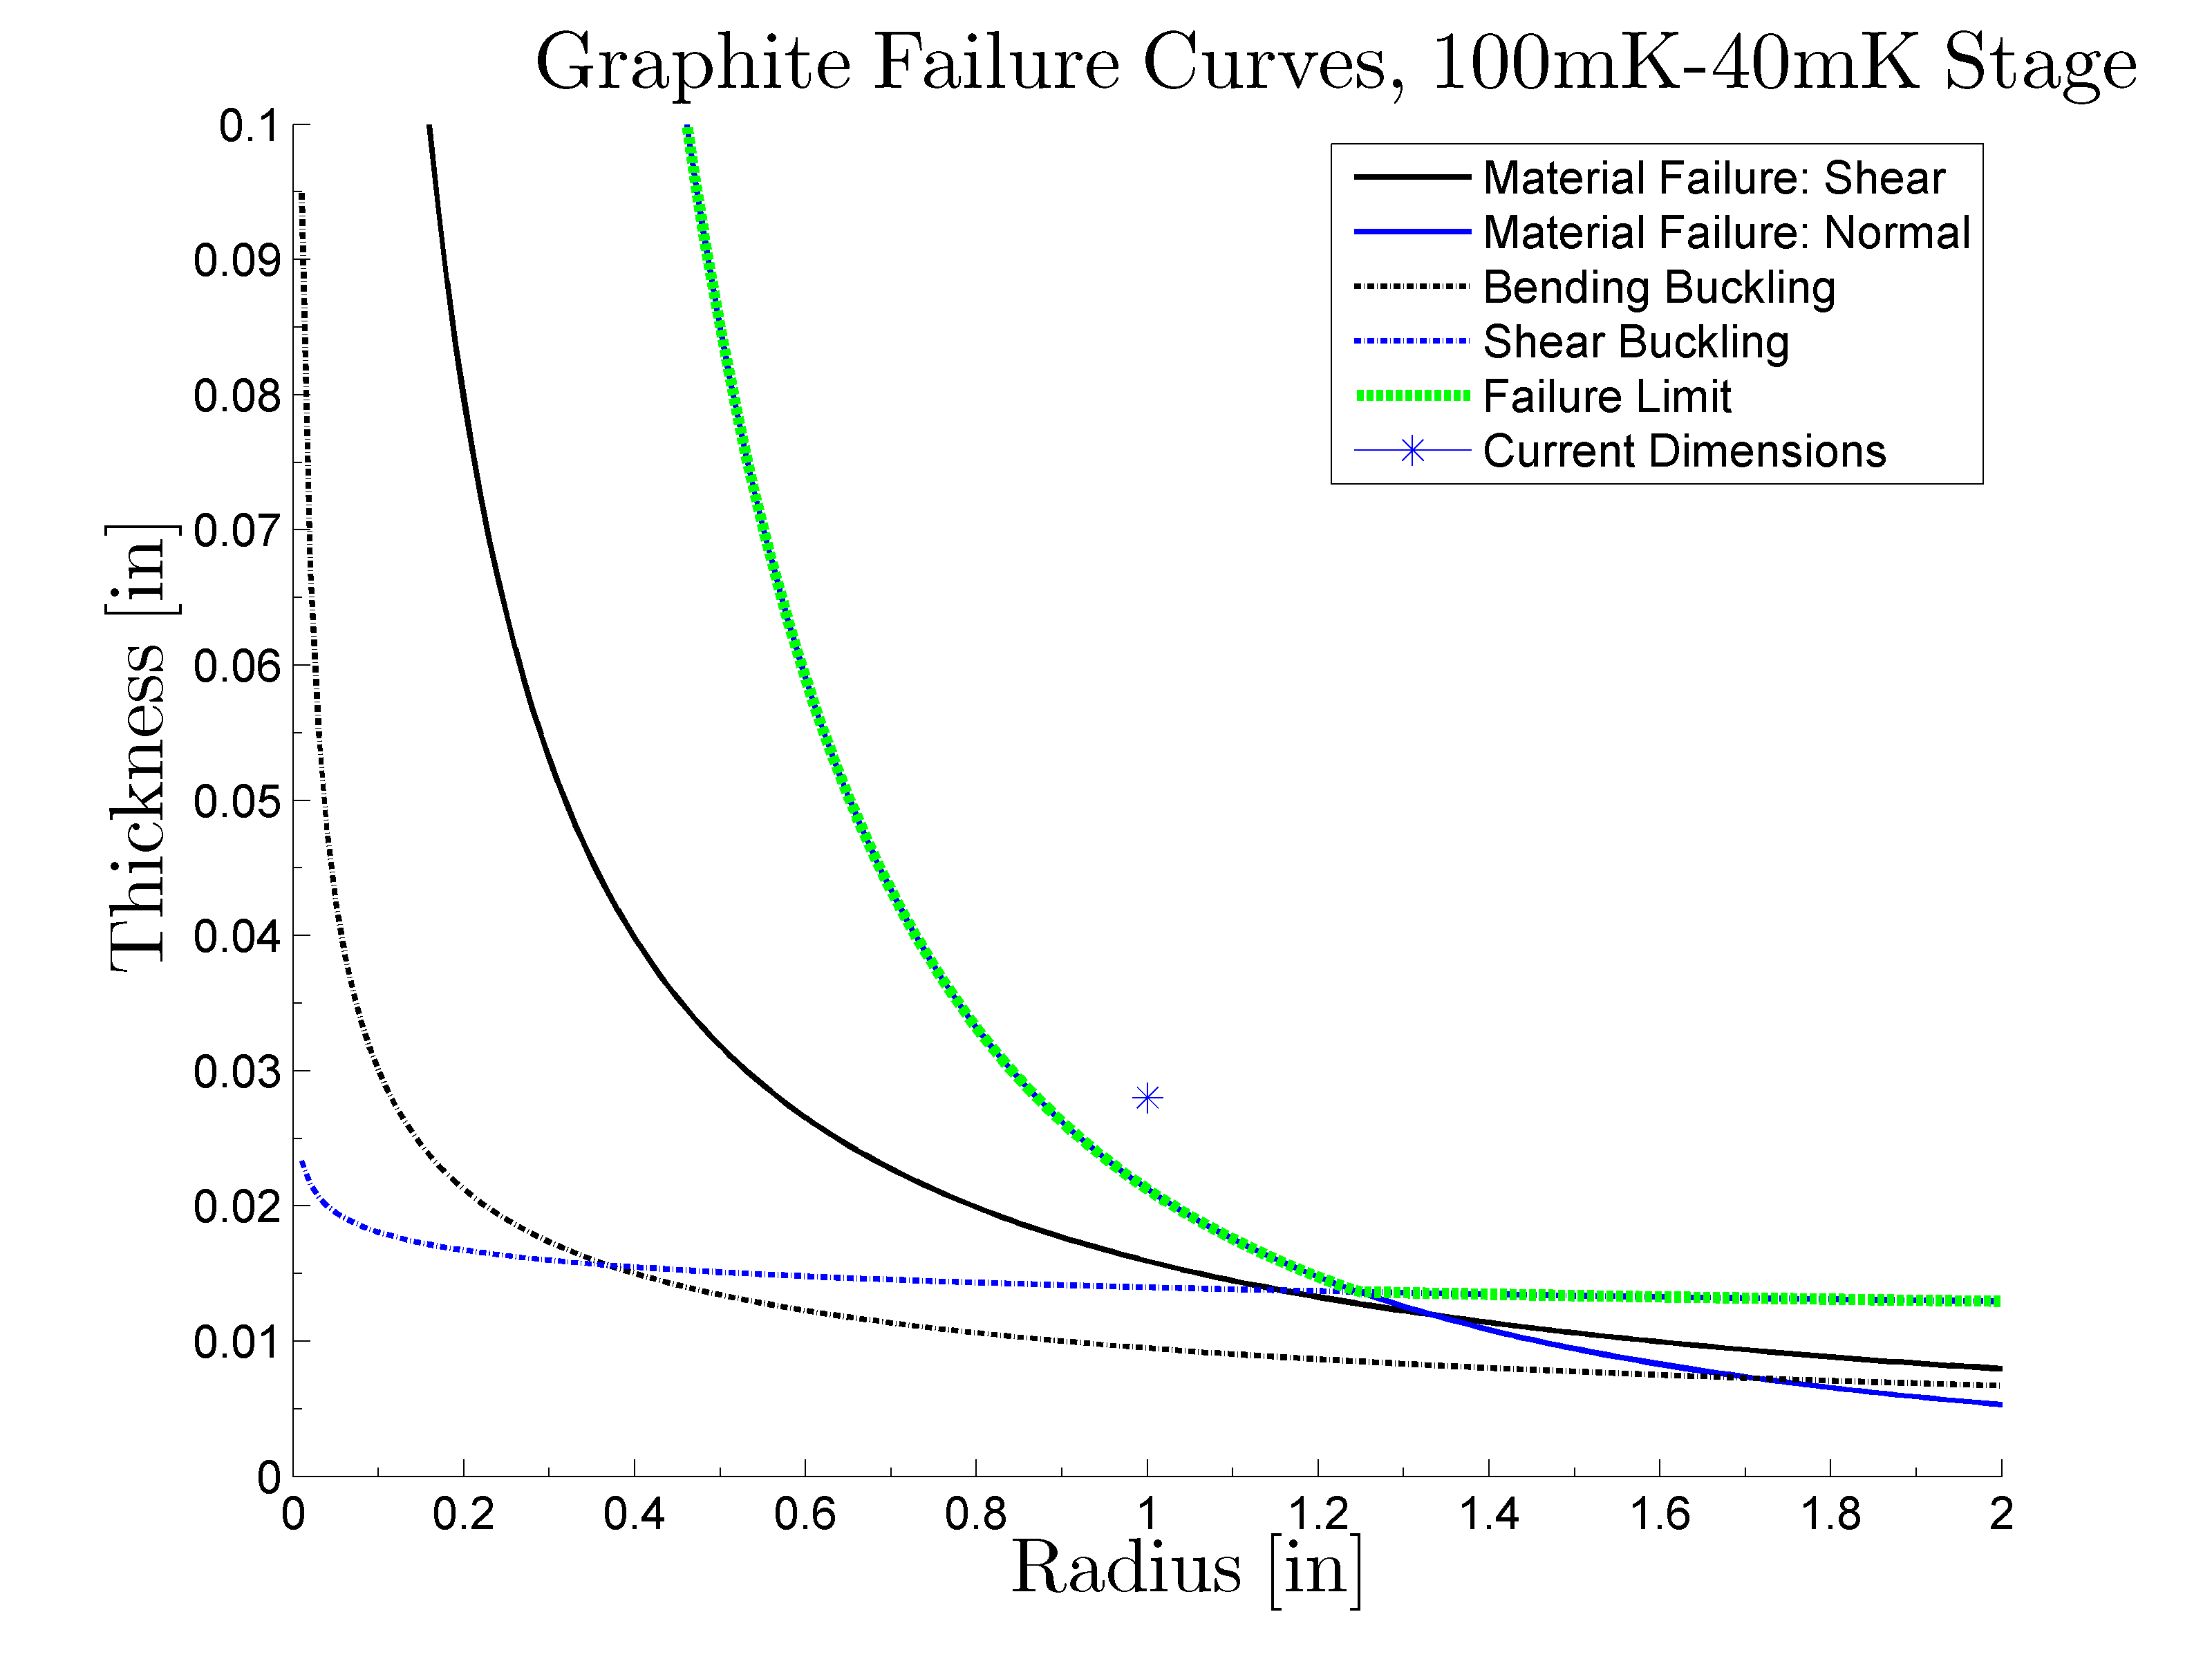
\includegraphics[width=\textwidth]{Graphite_Failure100mK40mK.png}
%\end{minipage}
%\begin{minipage}[t]{.45\textwidth}
%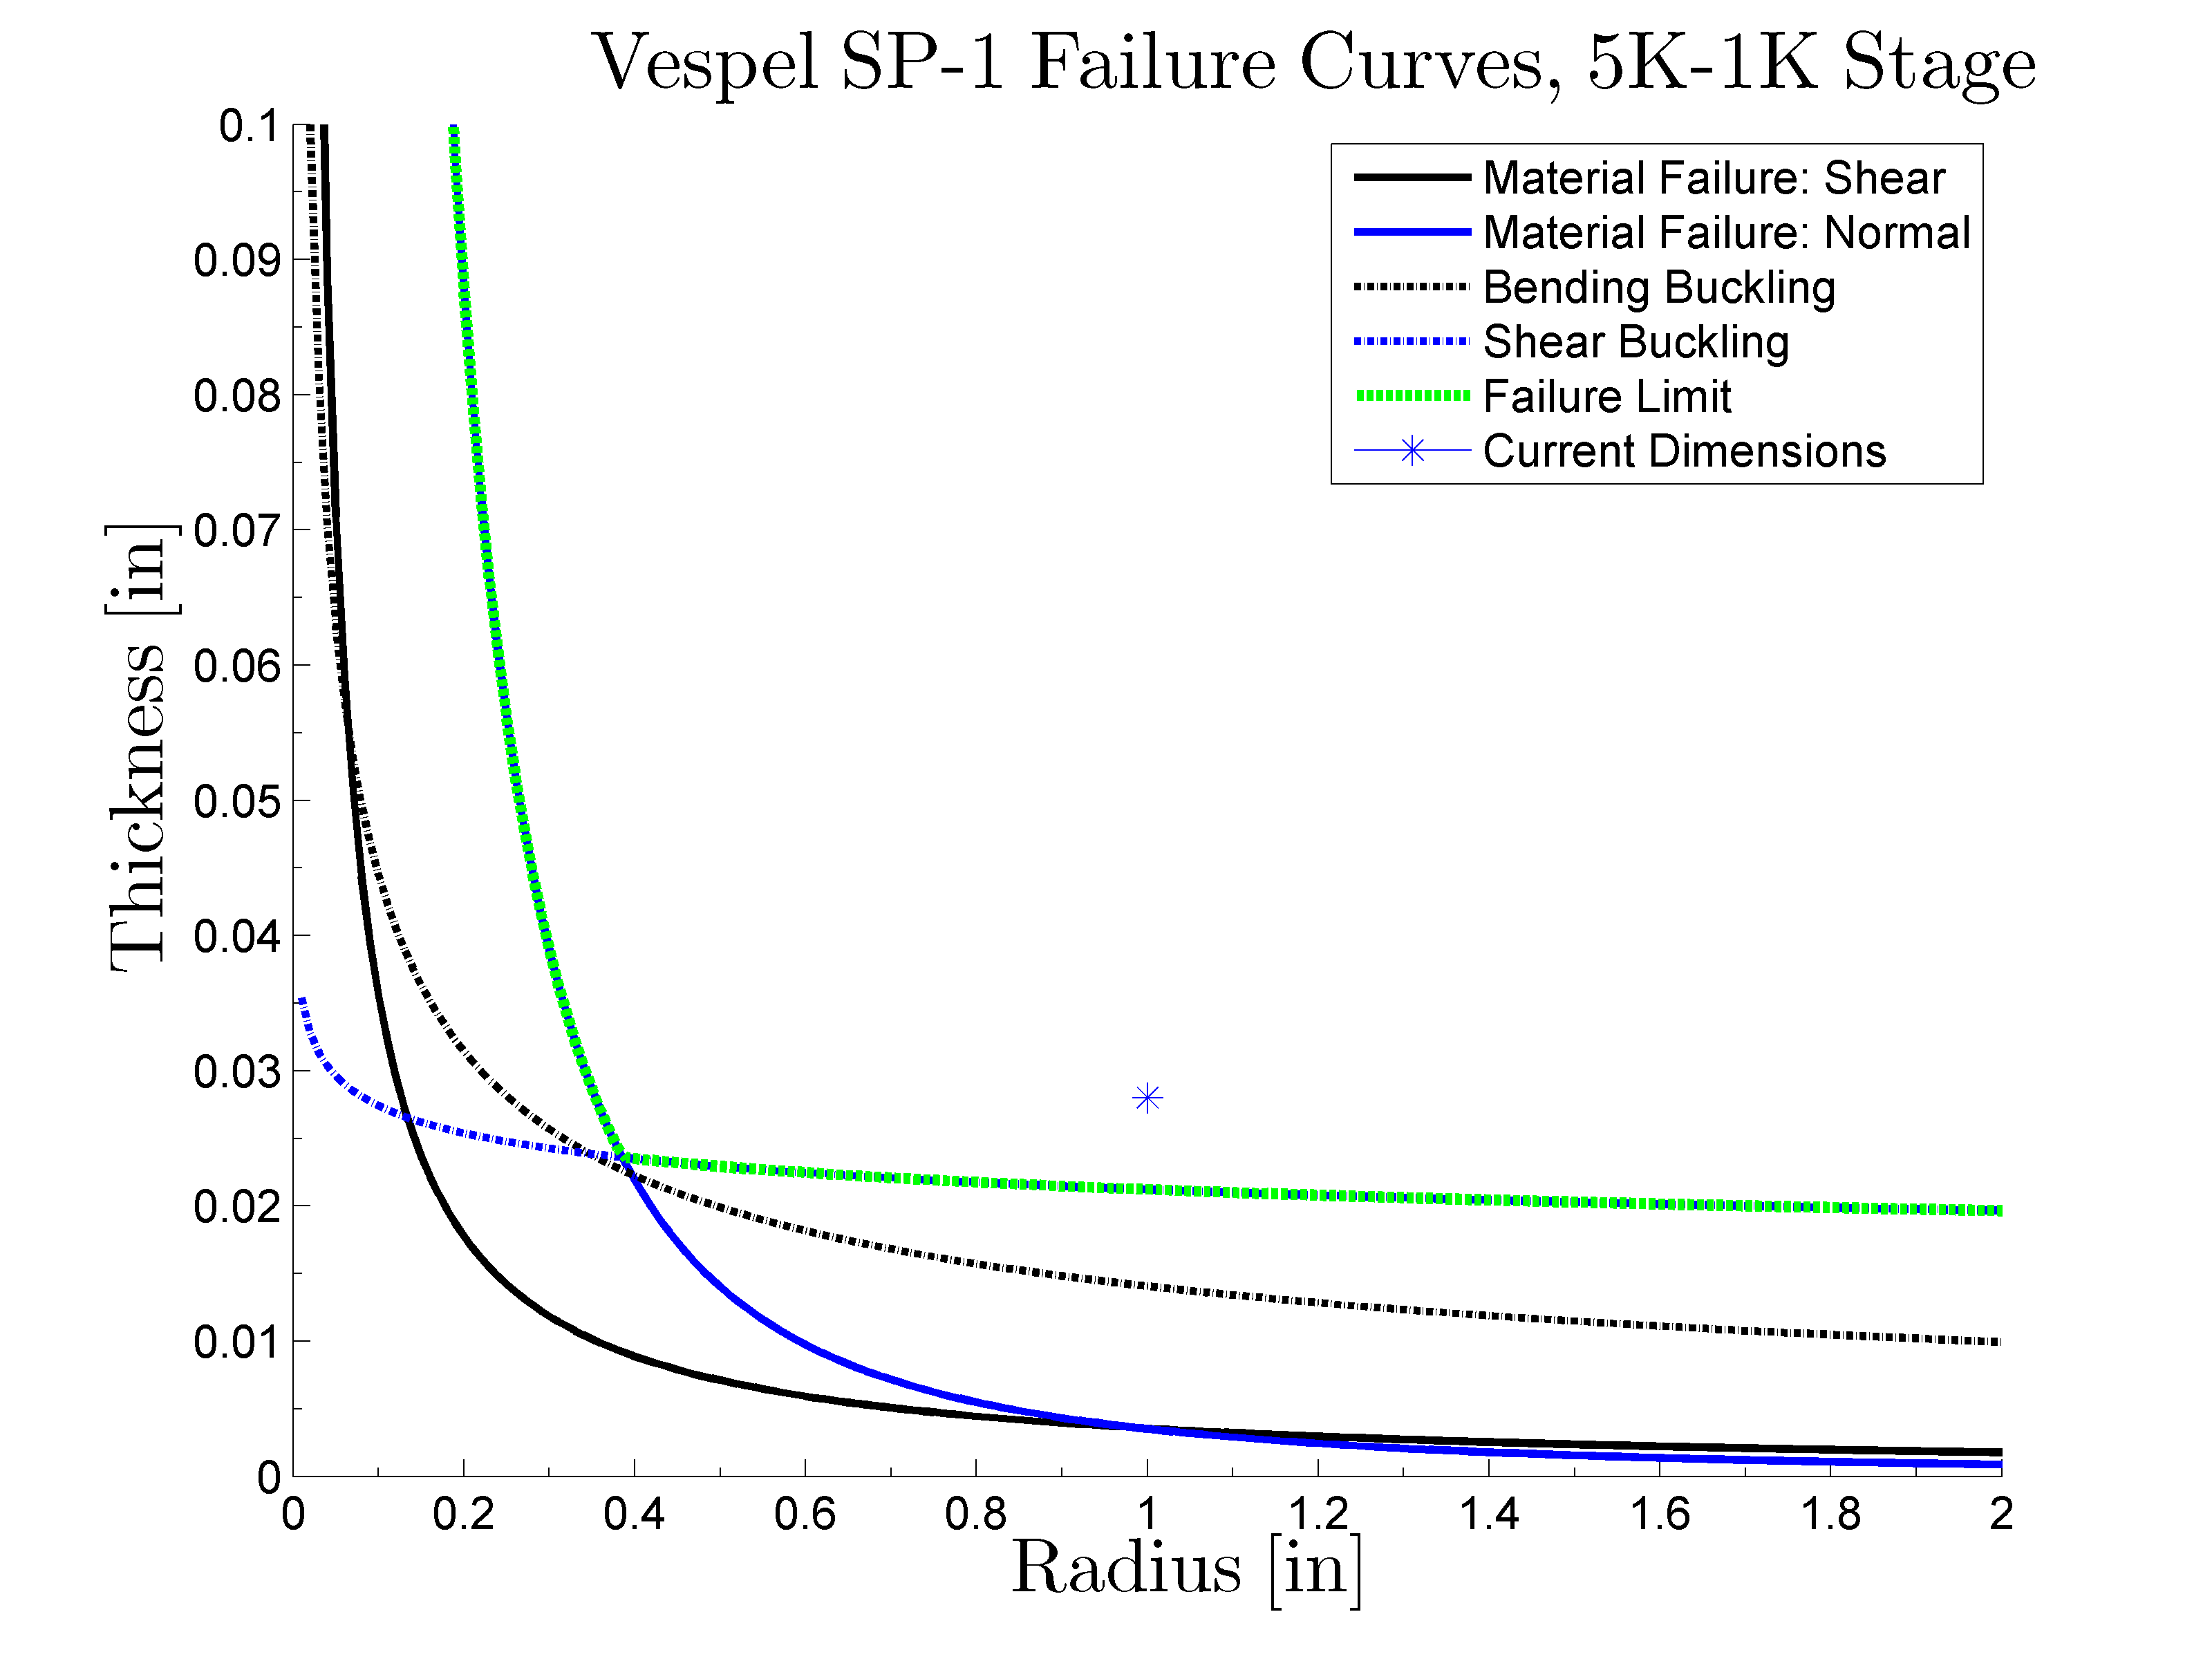
\includegraphics[width=\textwidth]{Vespel_Failure5K1K.png}
%\end{minipage}
%\end{figure}
%\begin{figure}[htb]
%\begin{minipage}[t]{.45\textwidth}
%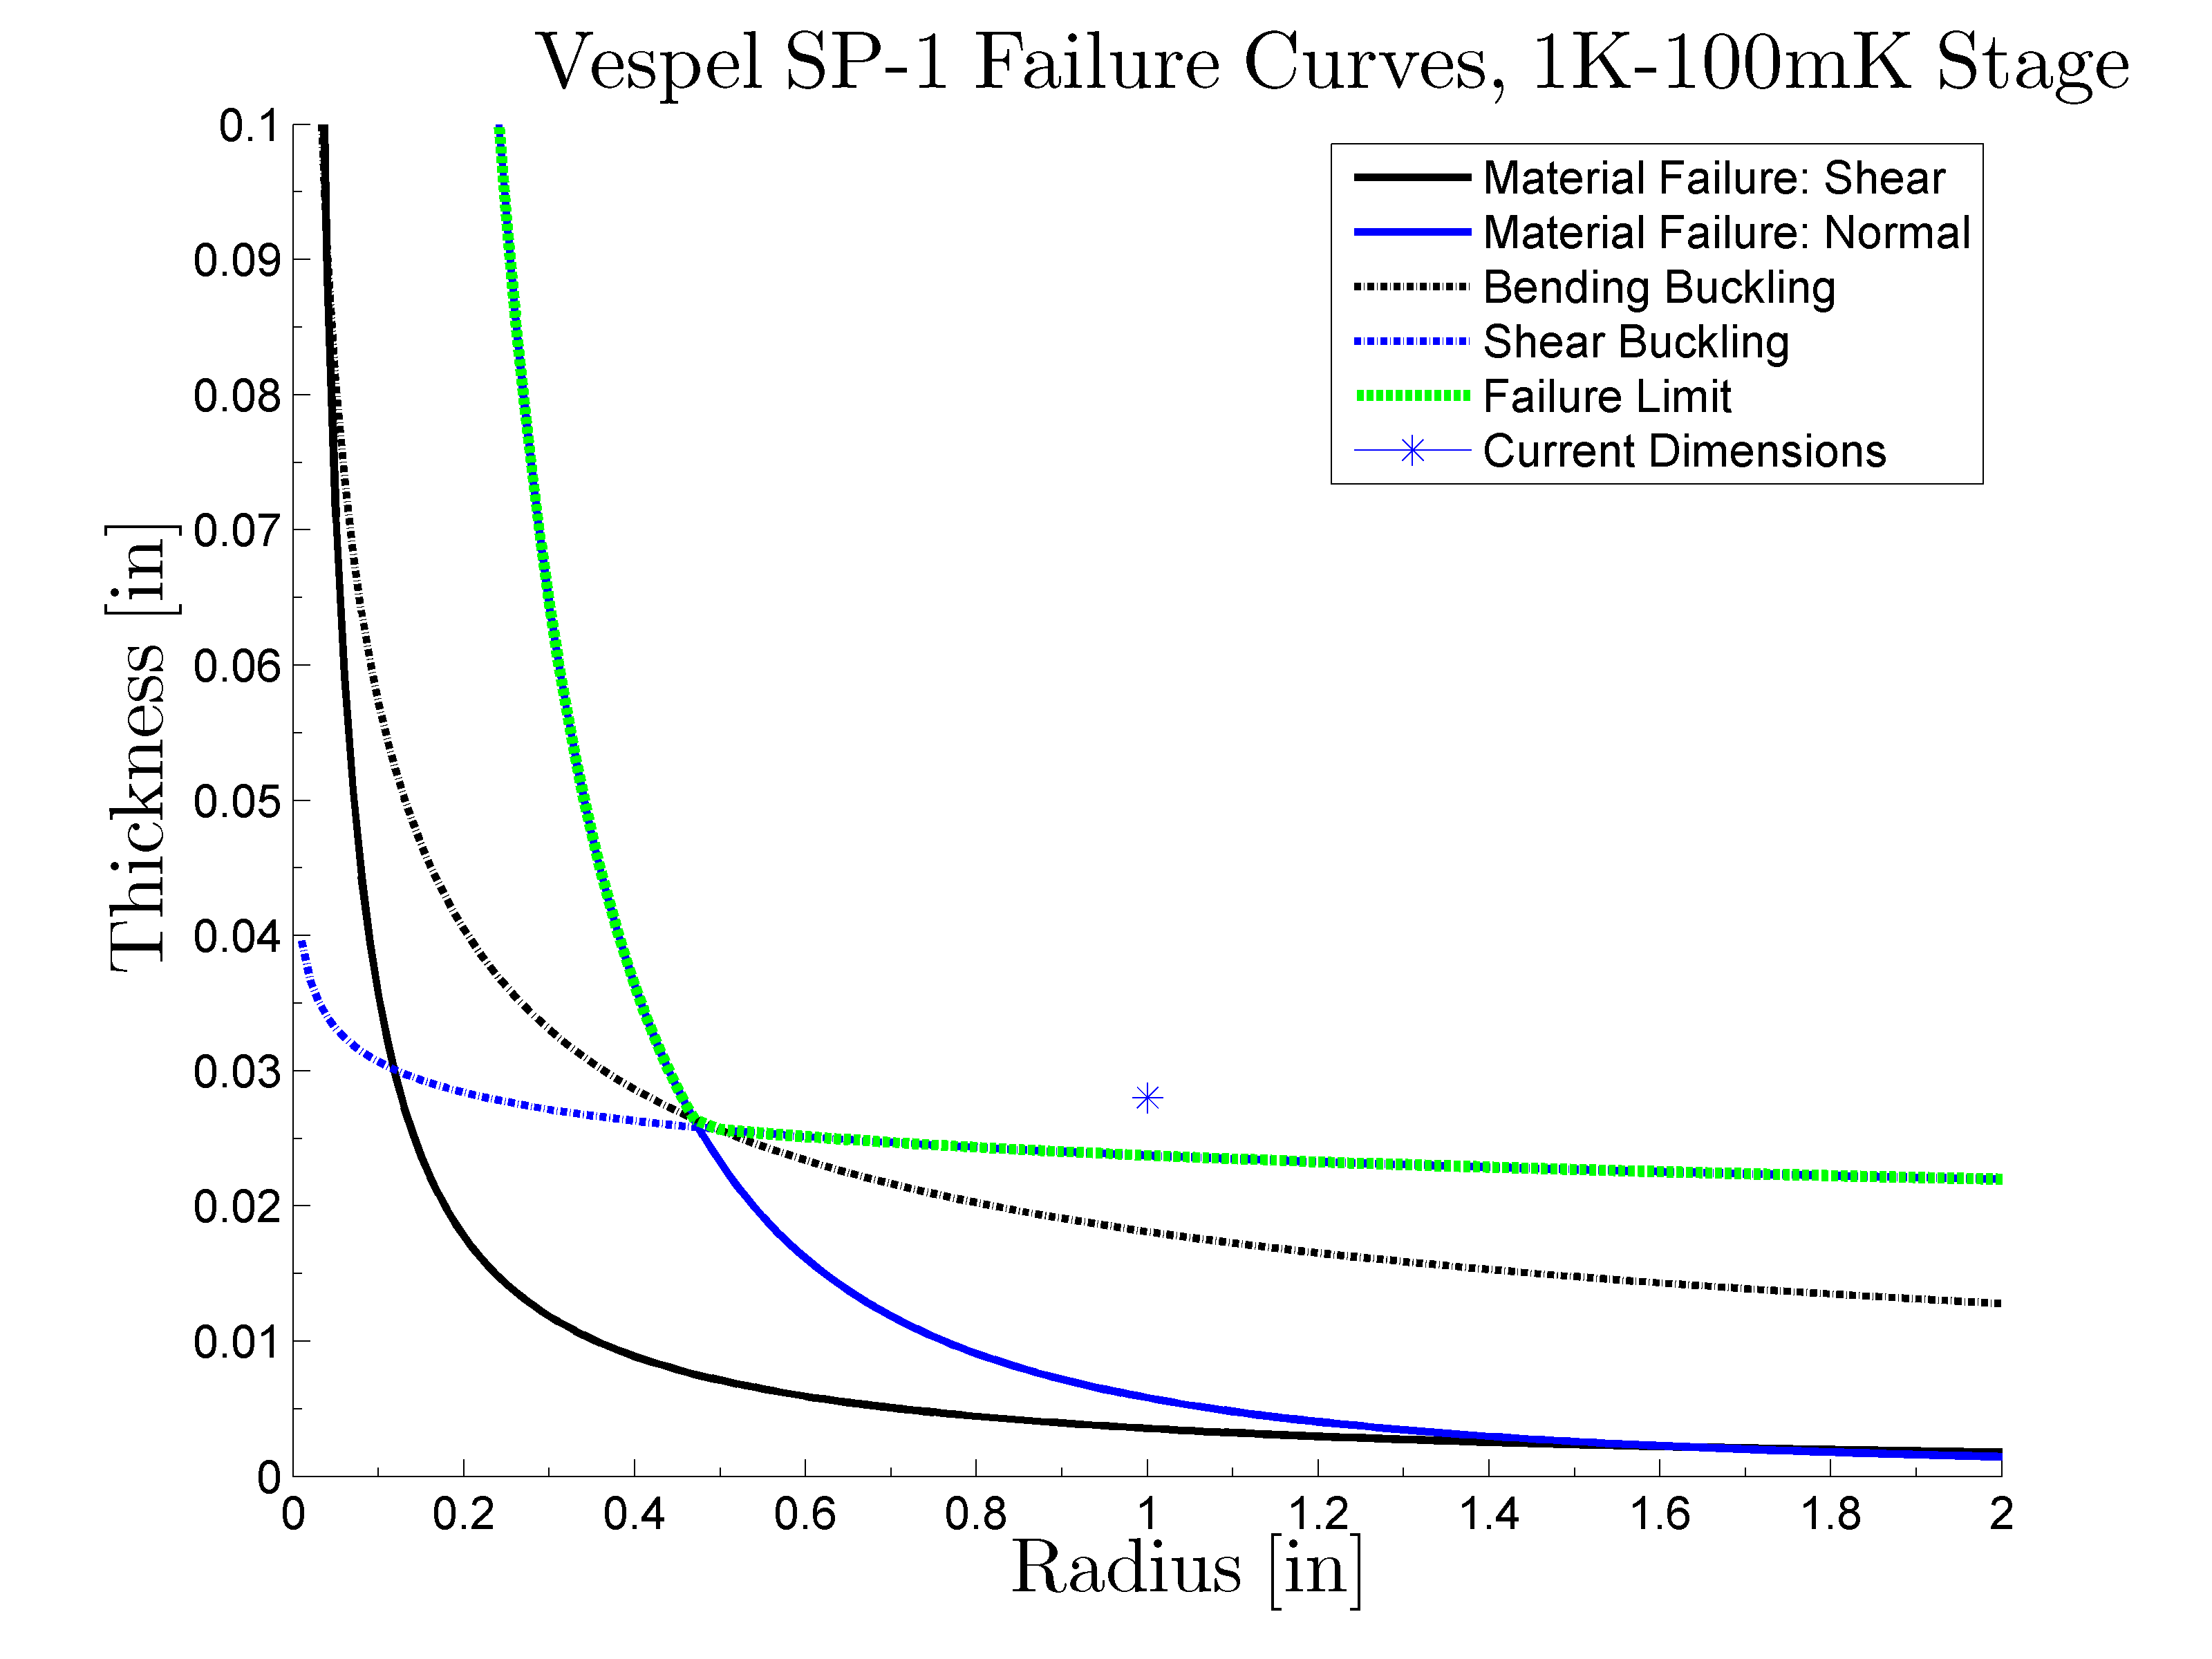
\includegraphics[width=\textwidth]{Vespel_Failure1K100mK.png}
%\end{minipage}
%\begin{minipage}[t]{.45\textwidth}
%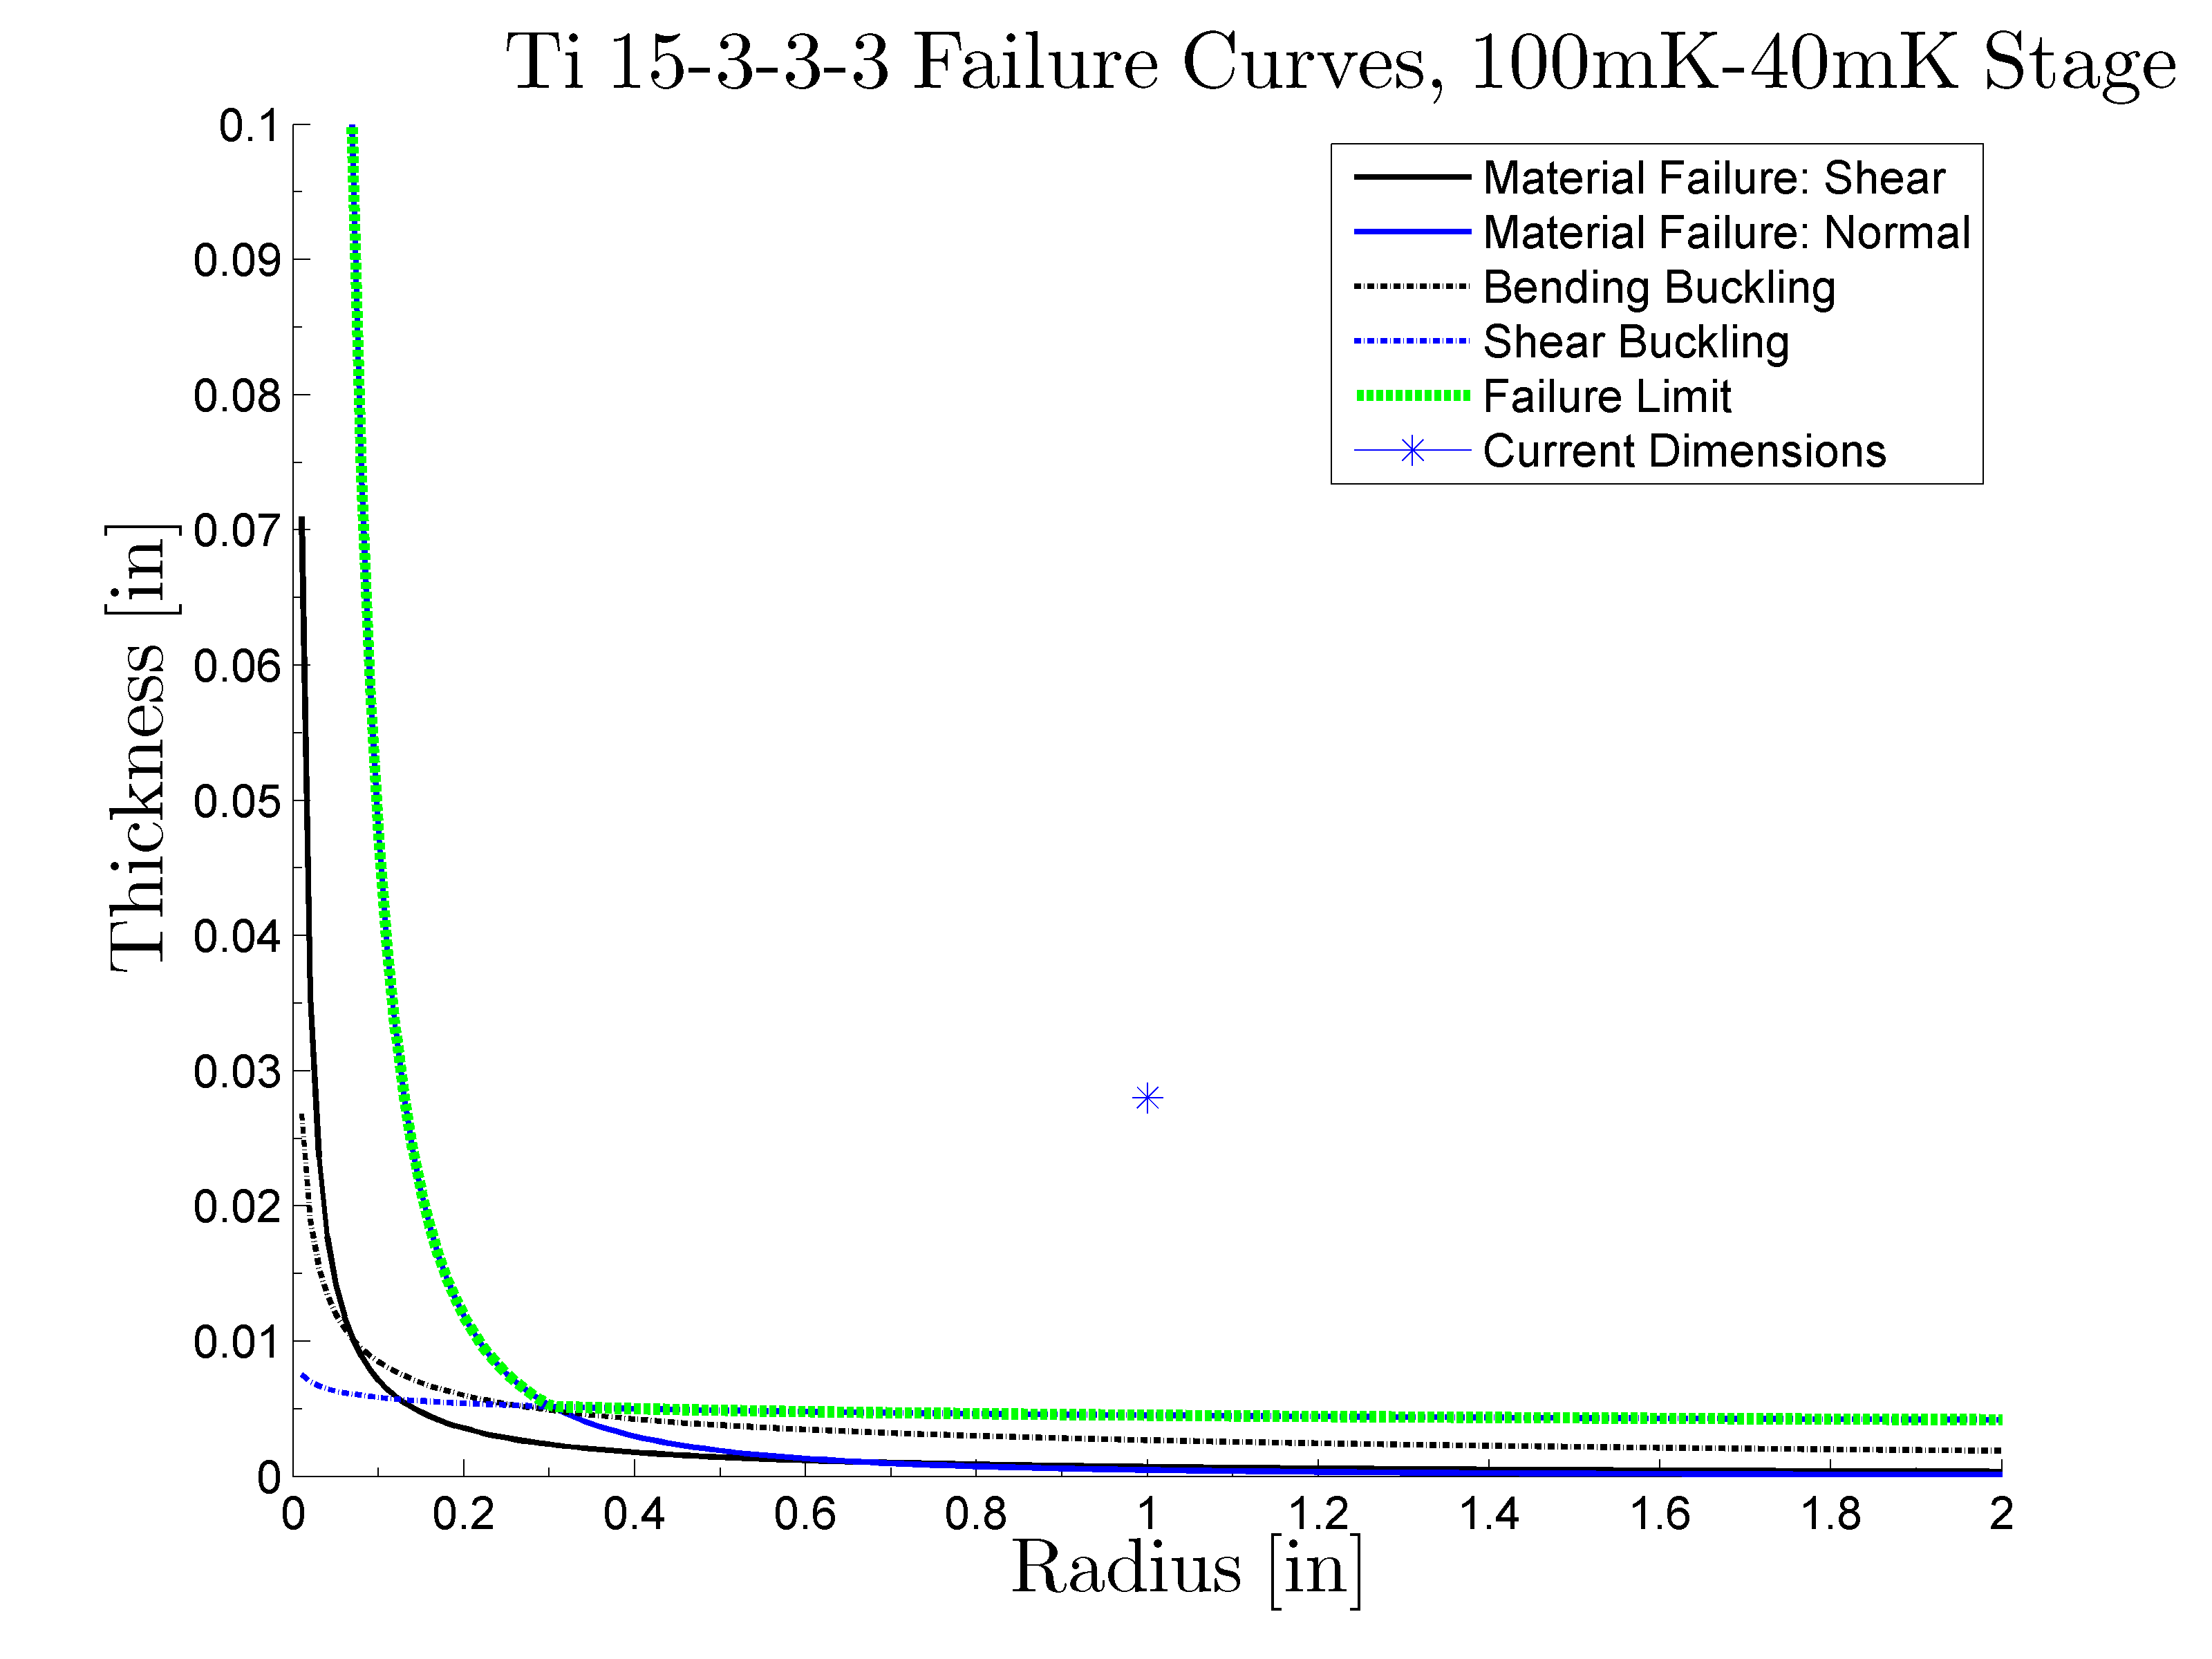
\includegraphics[width=\textwidth]{Ti15333_Failure.png}
%\end{minipage}
%\caption{Theoretical failure curves for different materials for 145lb load. The green dashed line represents minimum (thus optimum) dimensions for a 145lb load. Actual CDMS
%Graphite dimensions are plotted as an '*' for comparison.}
%\end{figure}

The predicted failure curves for CDMS graphite can be seen in the upper-left graph. The predicted dimensions for CDMS Graphite deviate $15-23\%$ from actual values of Radius = 1in, Thickness = 0.028in. The graphite model is still rough, however, as the values of tensile and compressive strength used were those approximated in table 3. These should be verified before further progress is made.

\subsection{Minimizing Radioactivity and Heat Load}

Once the optimal dimension pairs (radius, thickness) are obtained along the failure limit, we can minimize radioactivity and heat load of the candidate materials. Radioactivity is
directly proportional to volume, and thermal power is directly related to cross-sectional area. Holding tube lengths fixed, minimization of radioactivity and heat load is reduced
to the problem of minimizing cross-section. Therefore, radioactivity and heat load will have identical minimization parameters.

The graphs in figure 3 plot radioactivity and thermal power as a function of radius. The thickness of the tube at any radius is implicitly the thickness from the optimal dimension
pairs obtained from the failure limit lines in figure 2.

%\begin{figure}[htb]
%\begin{minipage}[t]{.48\textwidth}
%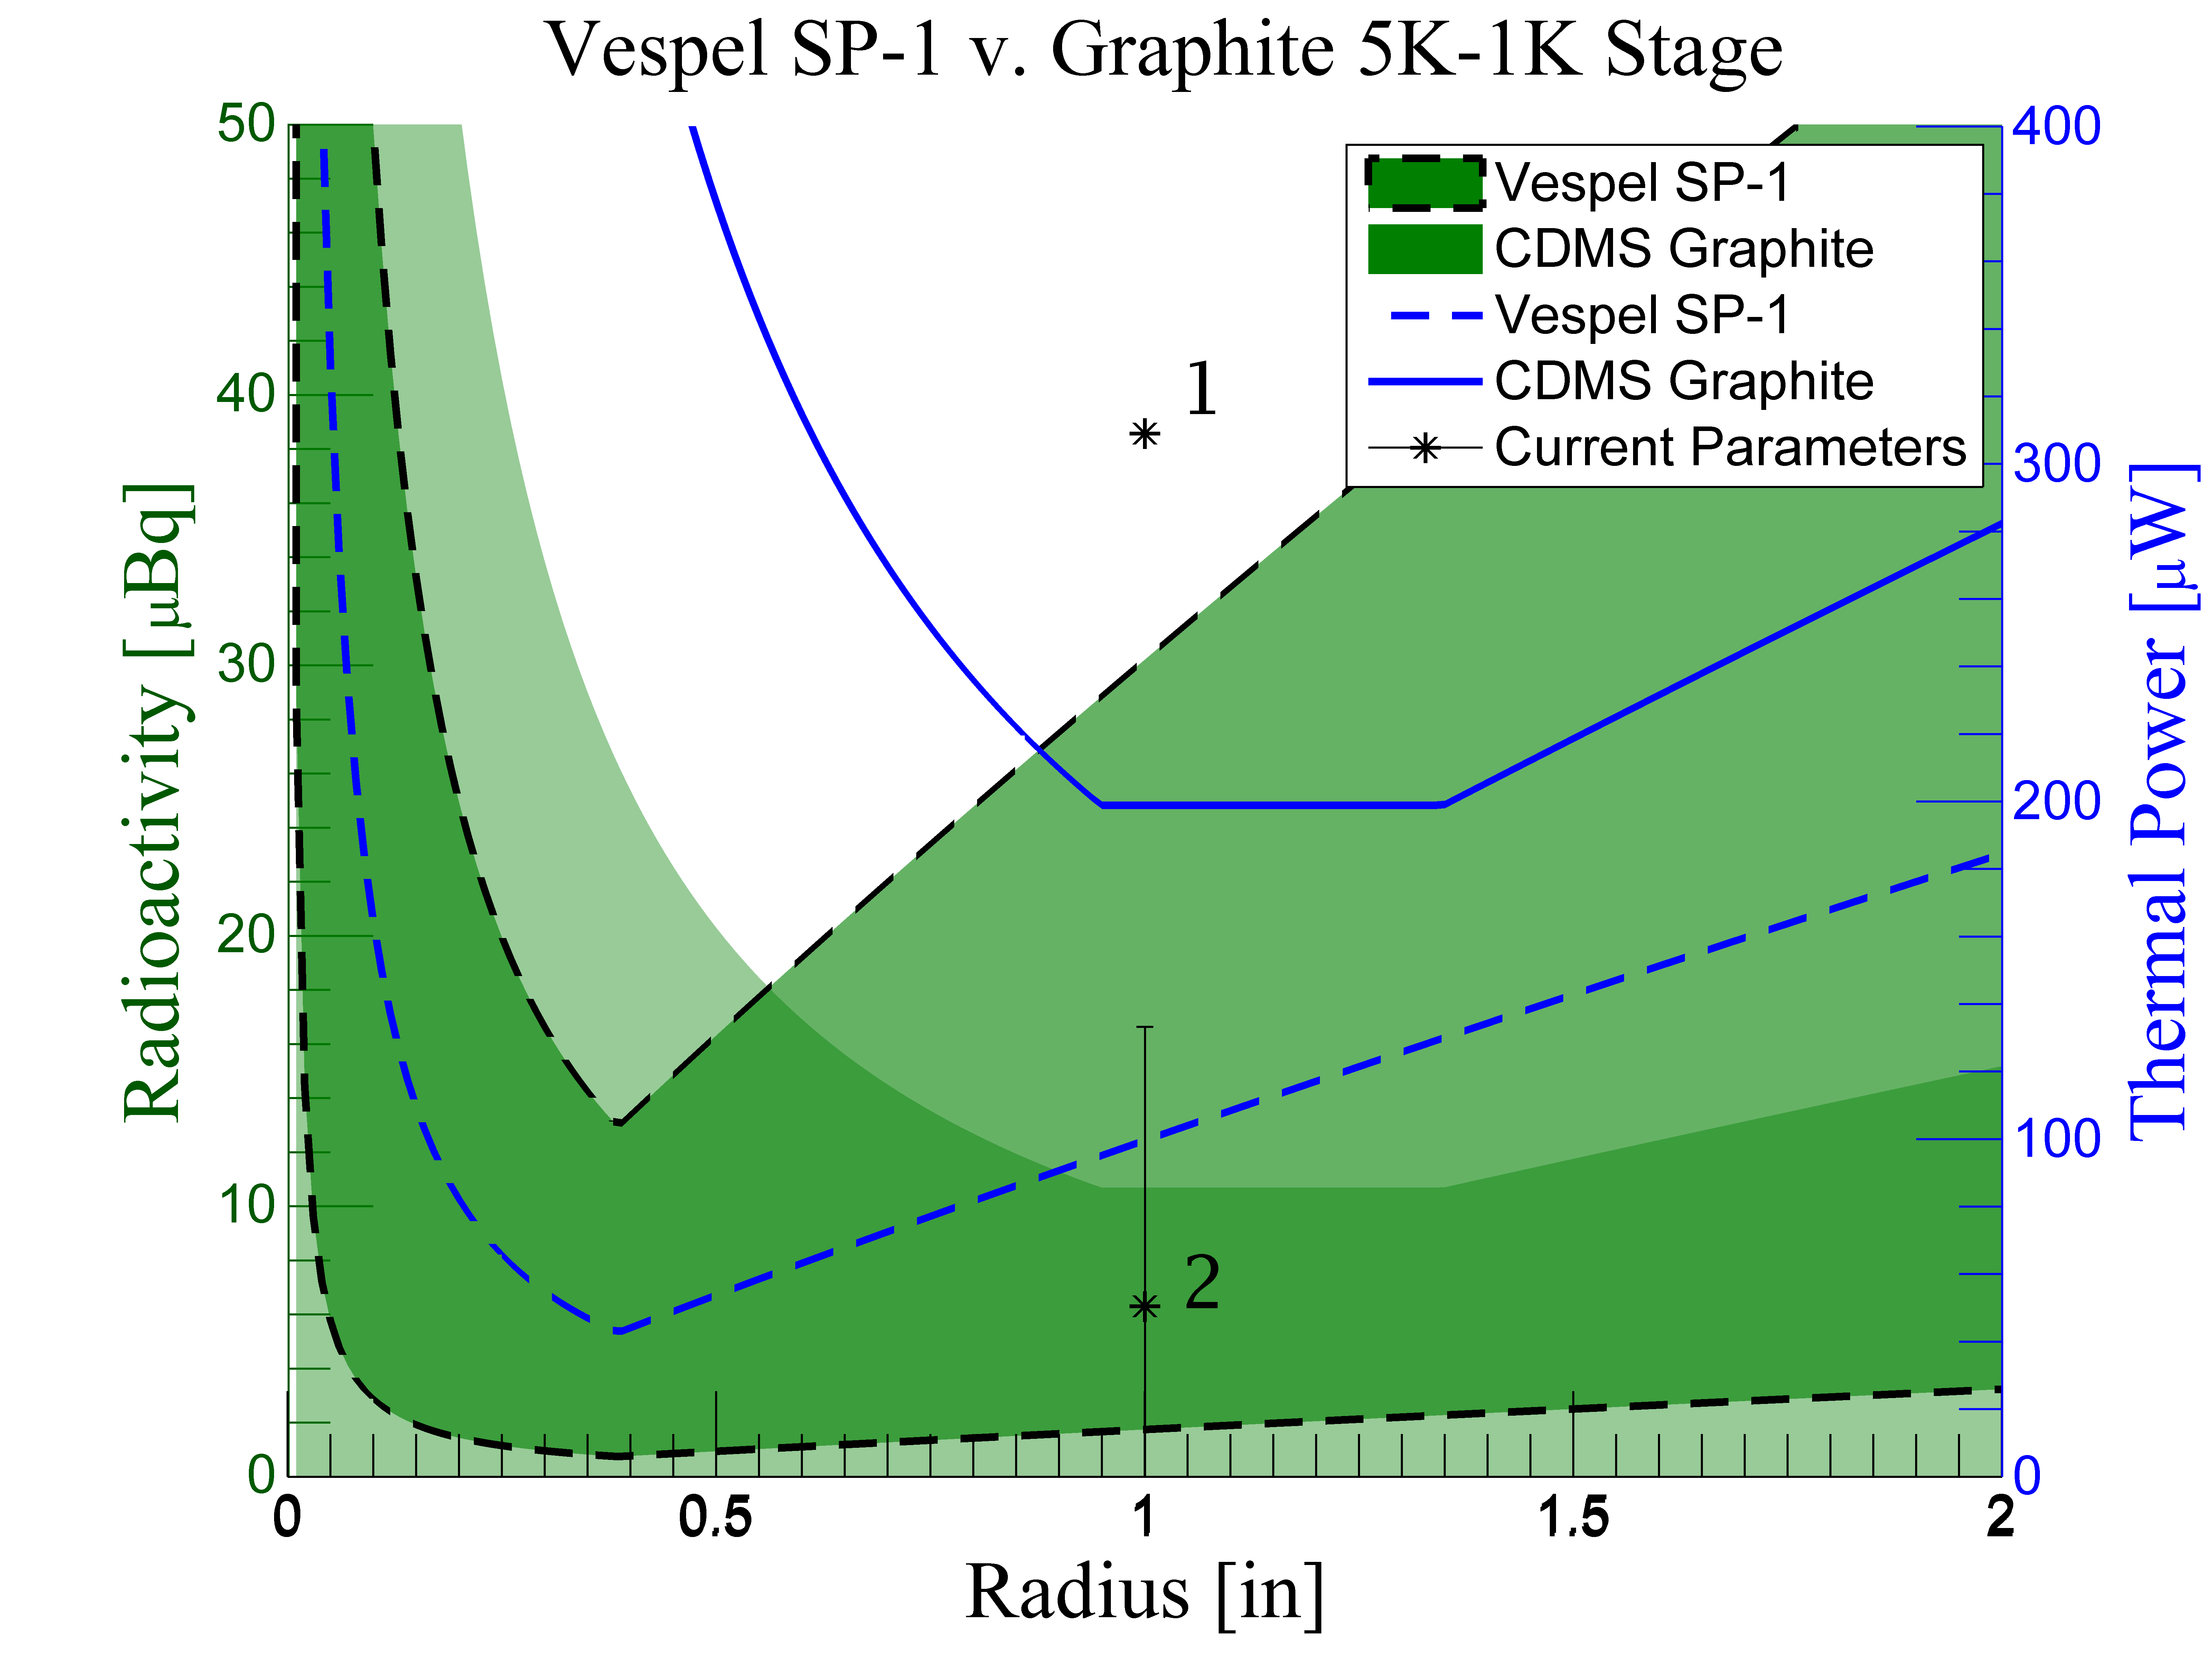
\includegraphics[width=\textwidth]{VSP1_Graphite_5K1K.png}
%\end{minipage}
%\begin{minipage}[t]{.48\textwidth}
%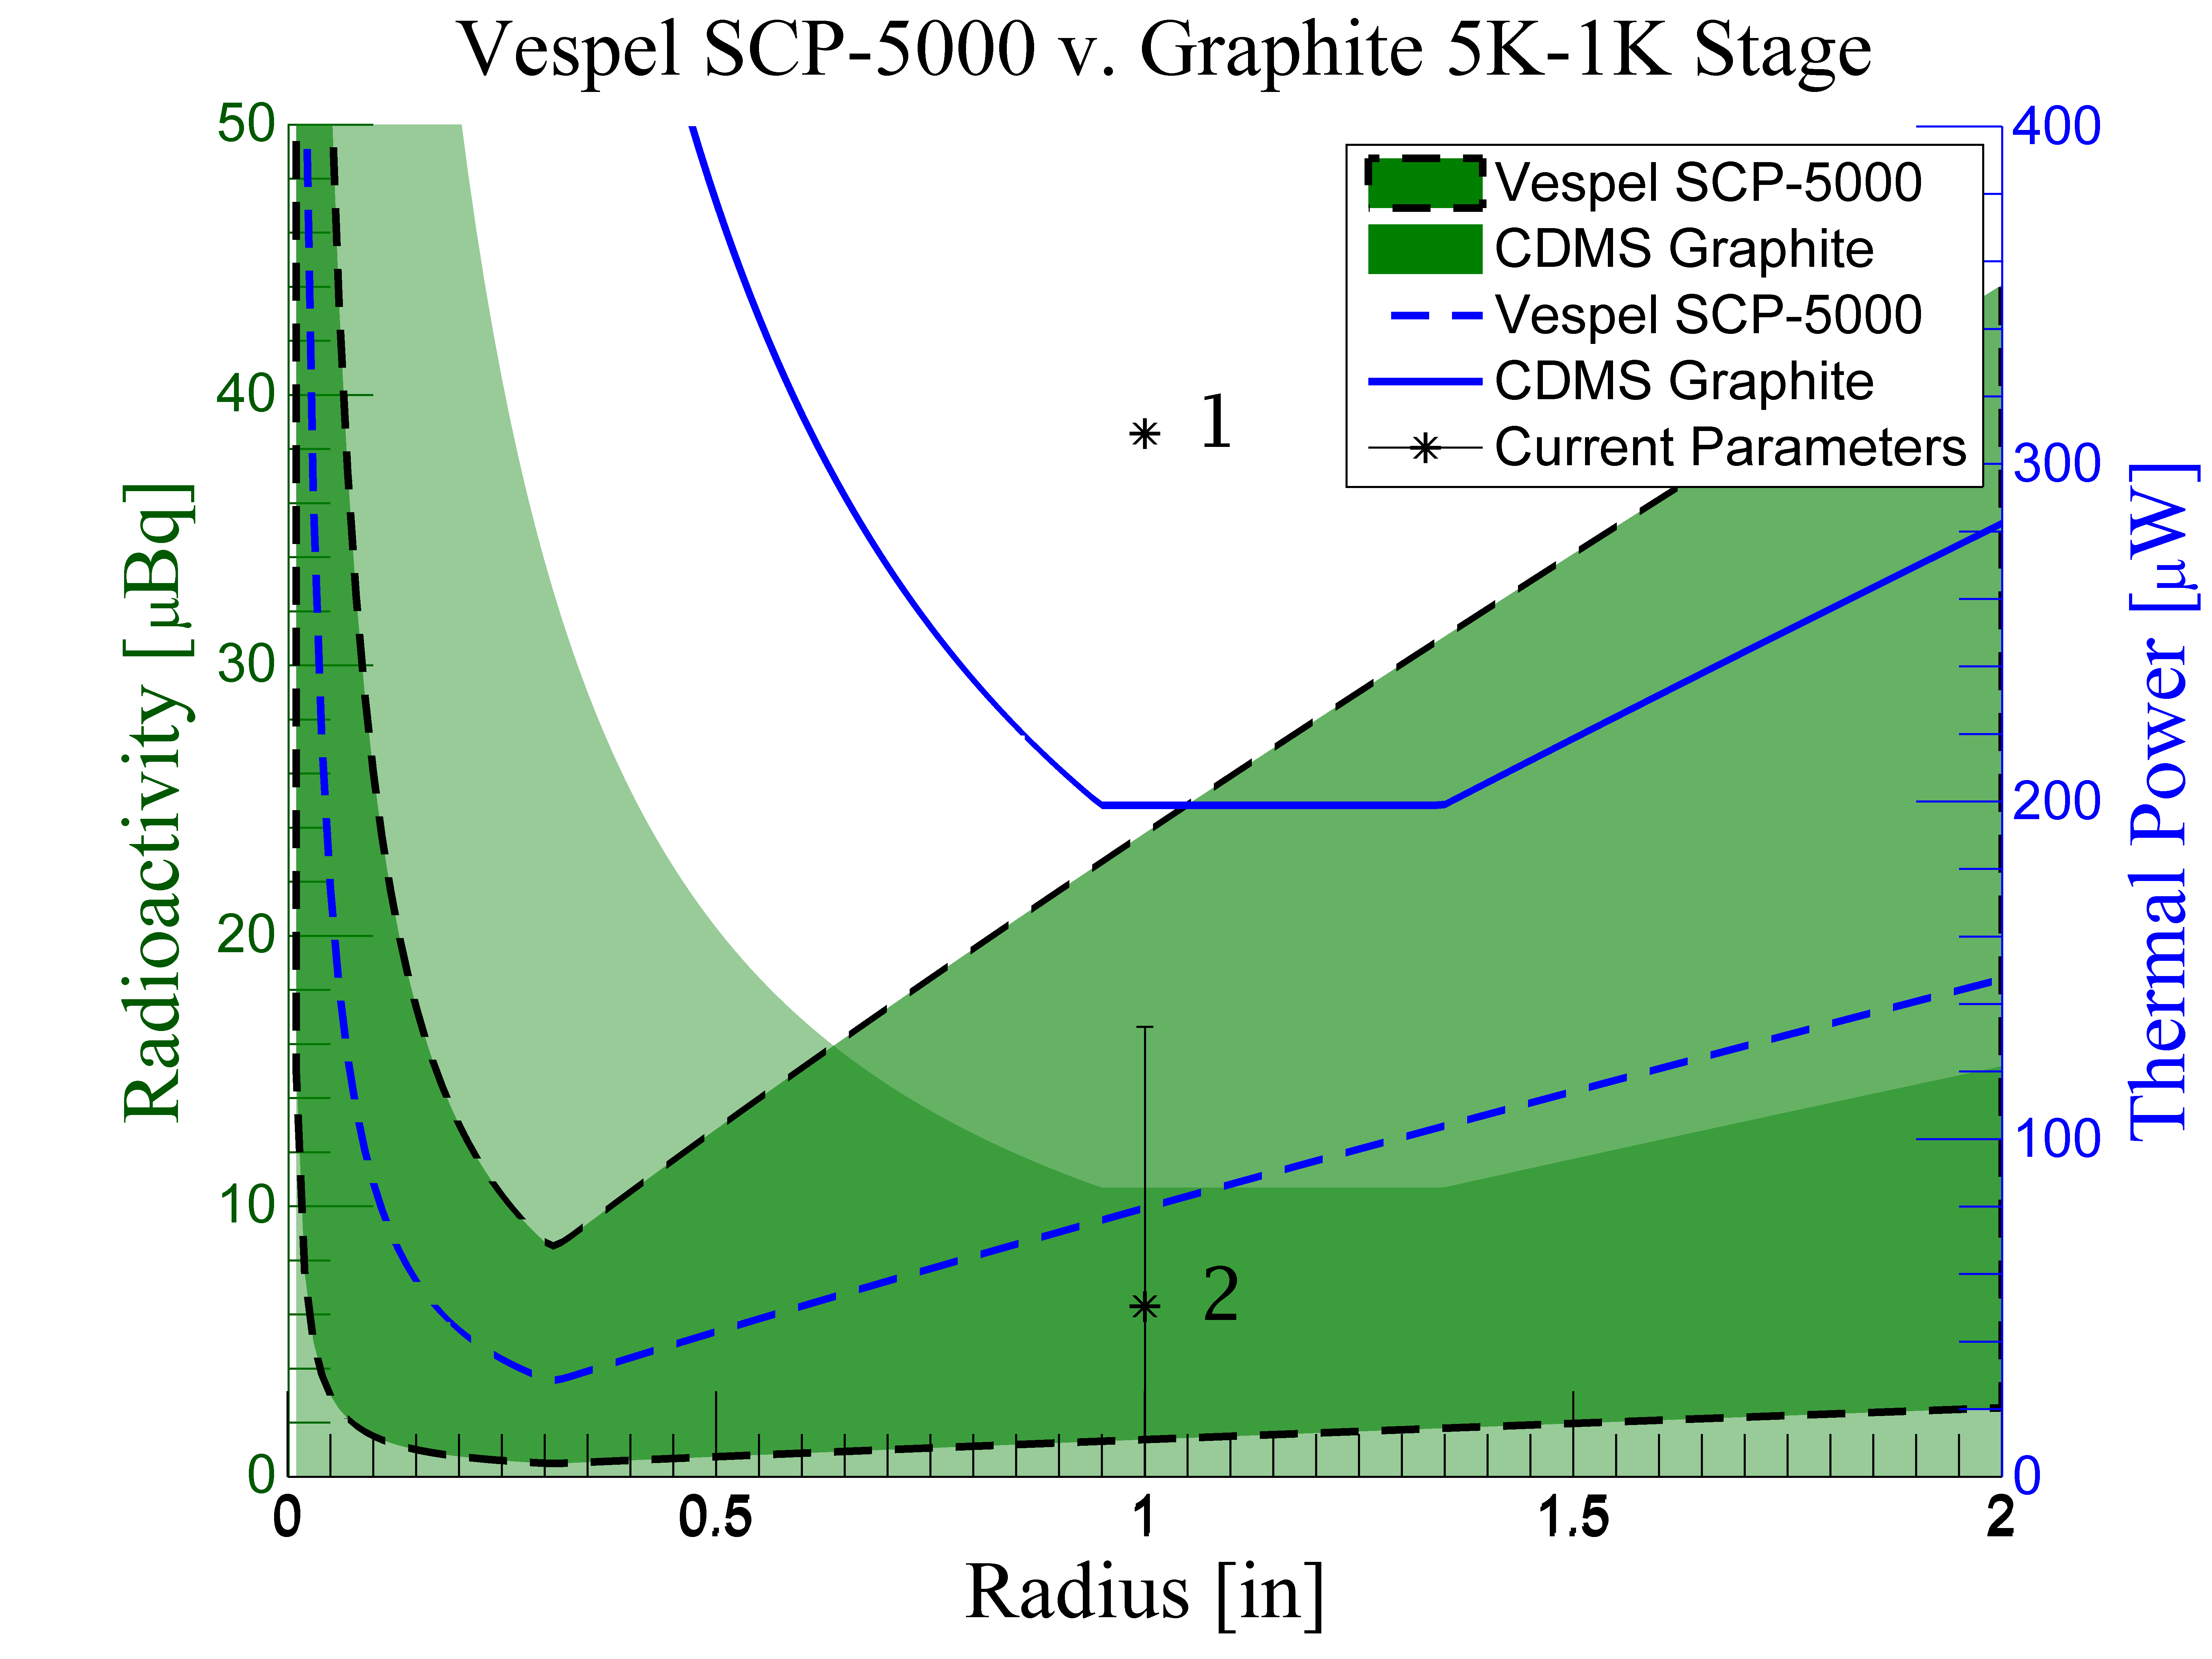
\includegraphics[width=\textwidth]{VSCP5000_Graphite_5K1K.png}
%\end{minipage}
%\end{figure}
%\begin{figure}[htb]
%\begin{minipage}[t]{.48\textwidth}
%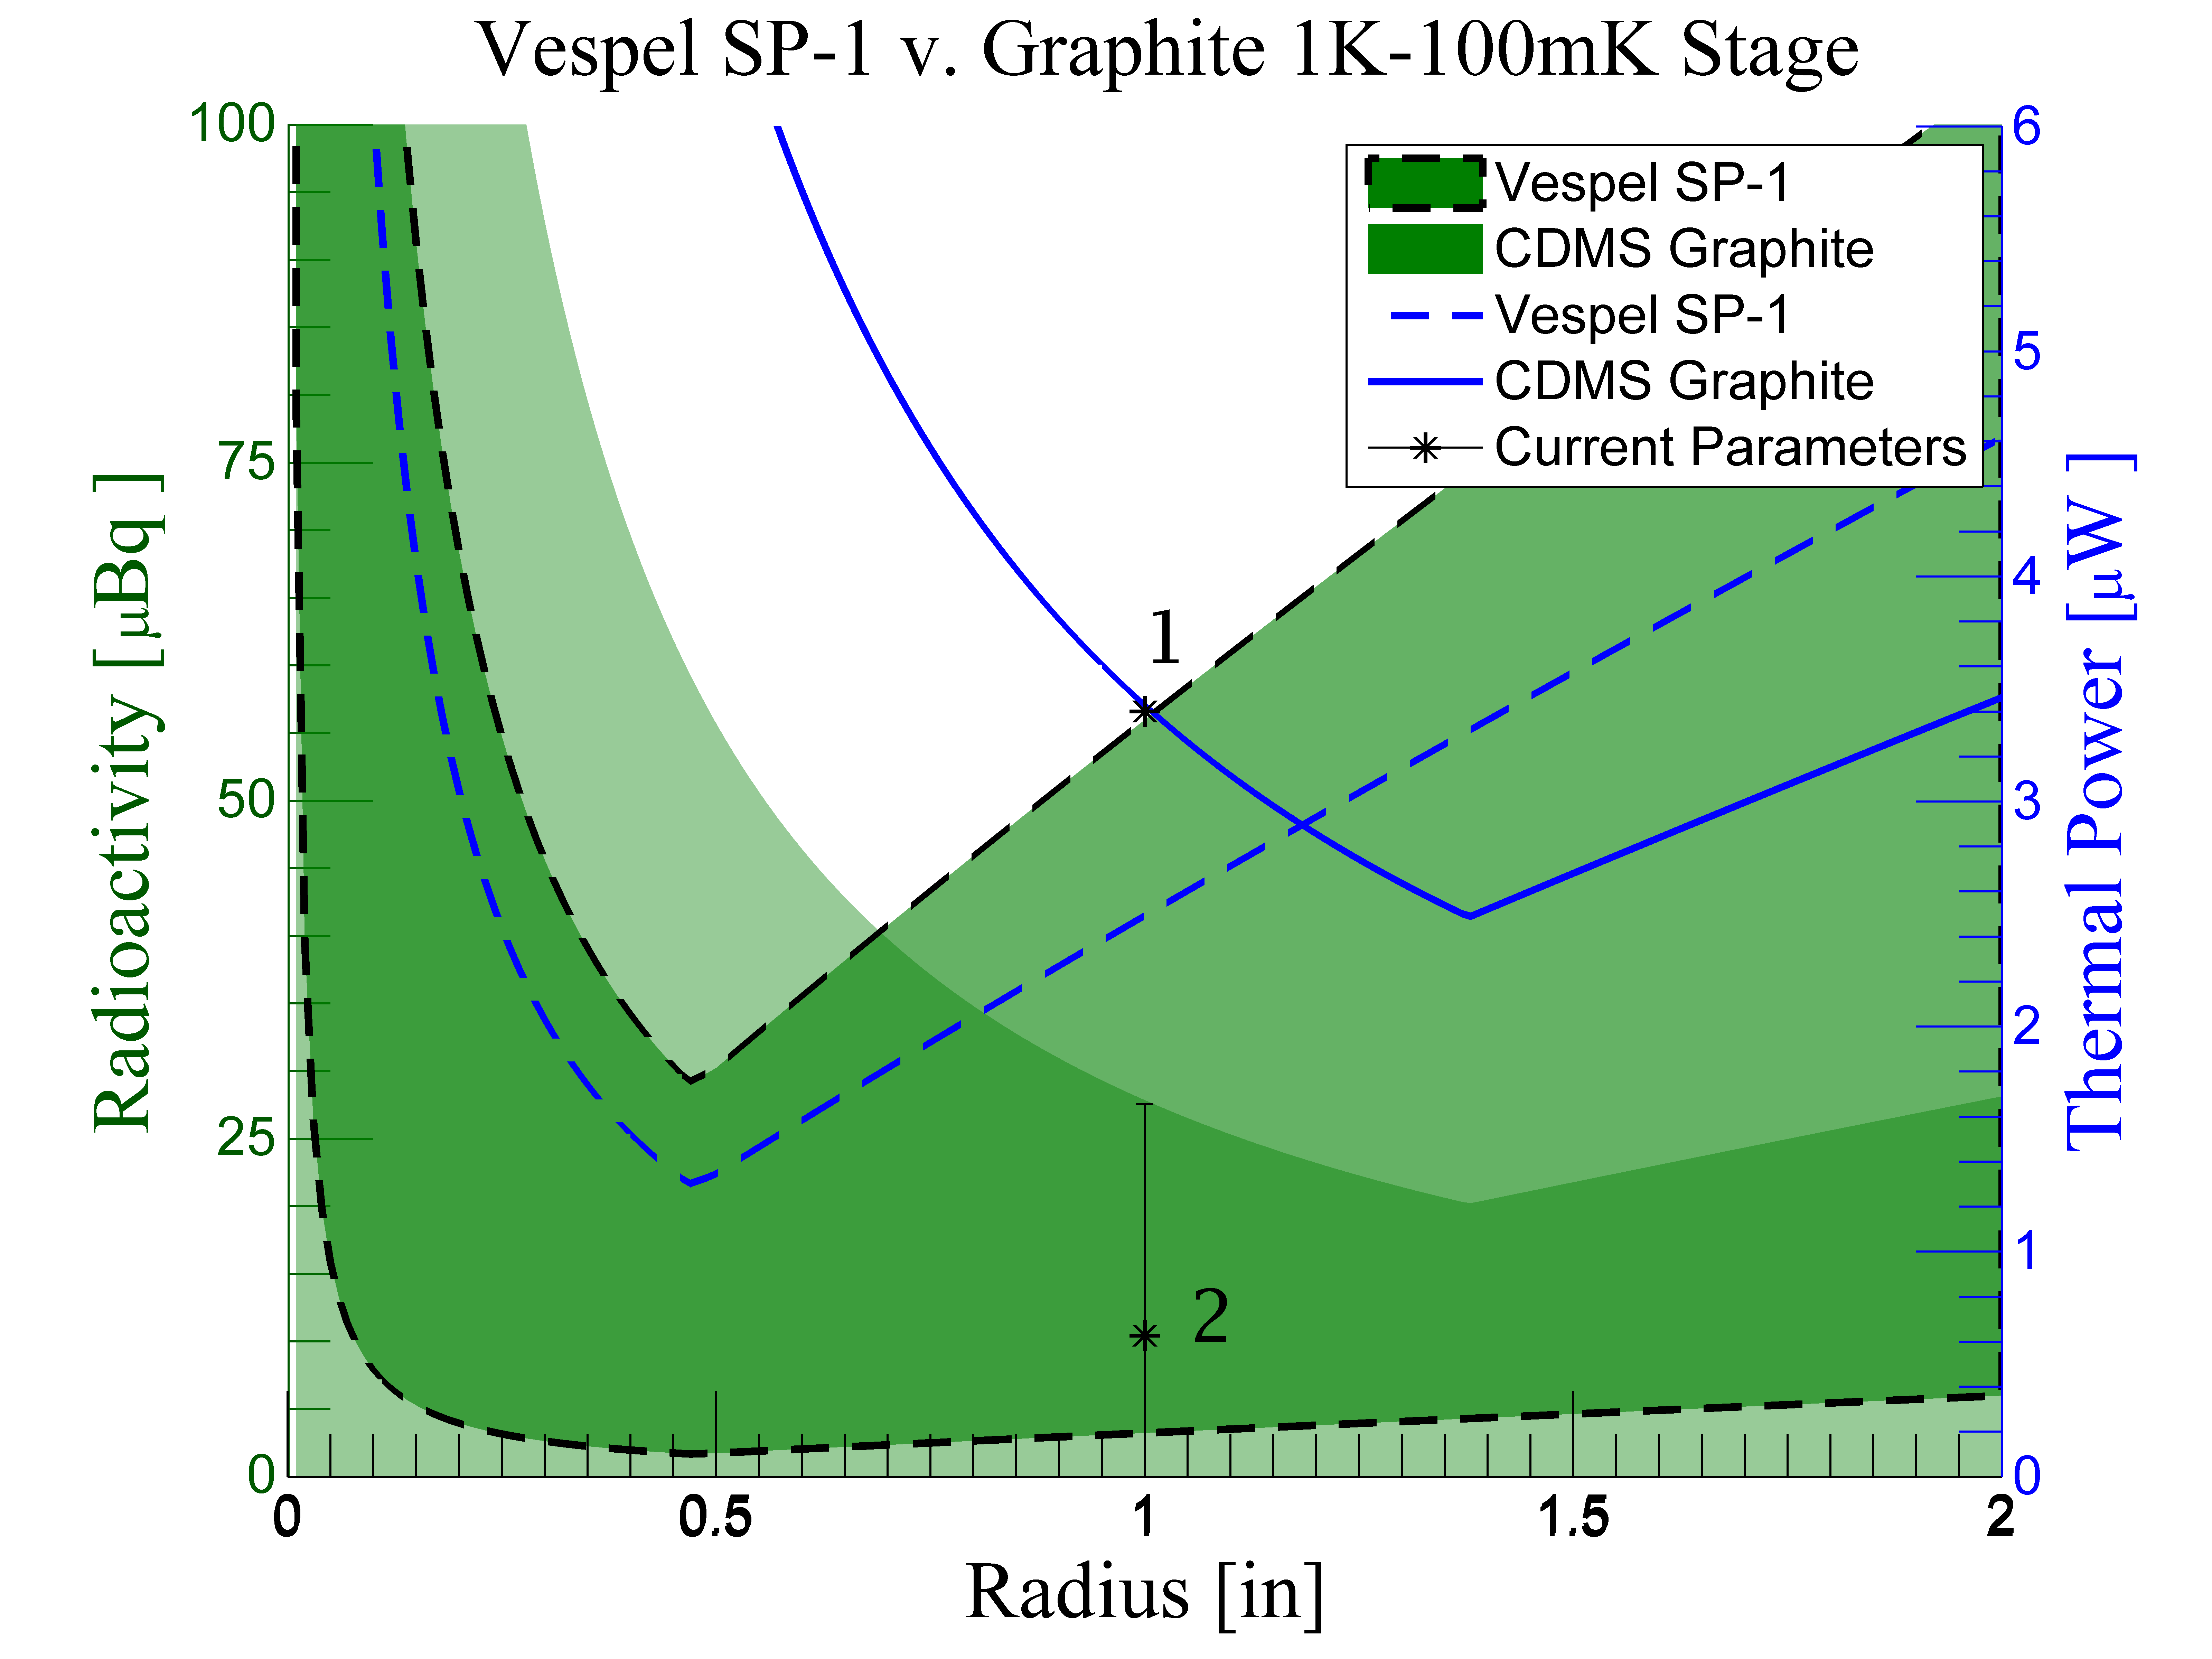
\includegraphics[width=\textwidth]{VSP1_Graphite_1K100mK.png}
%\end{minipage}
%\begin{minipage}[t]{.48\textwidth}
%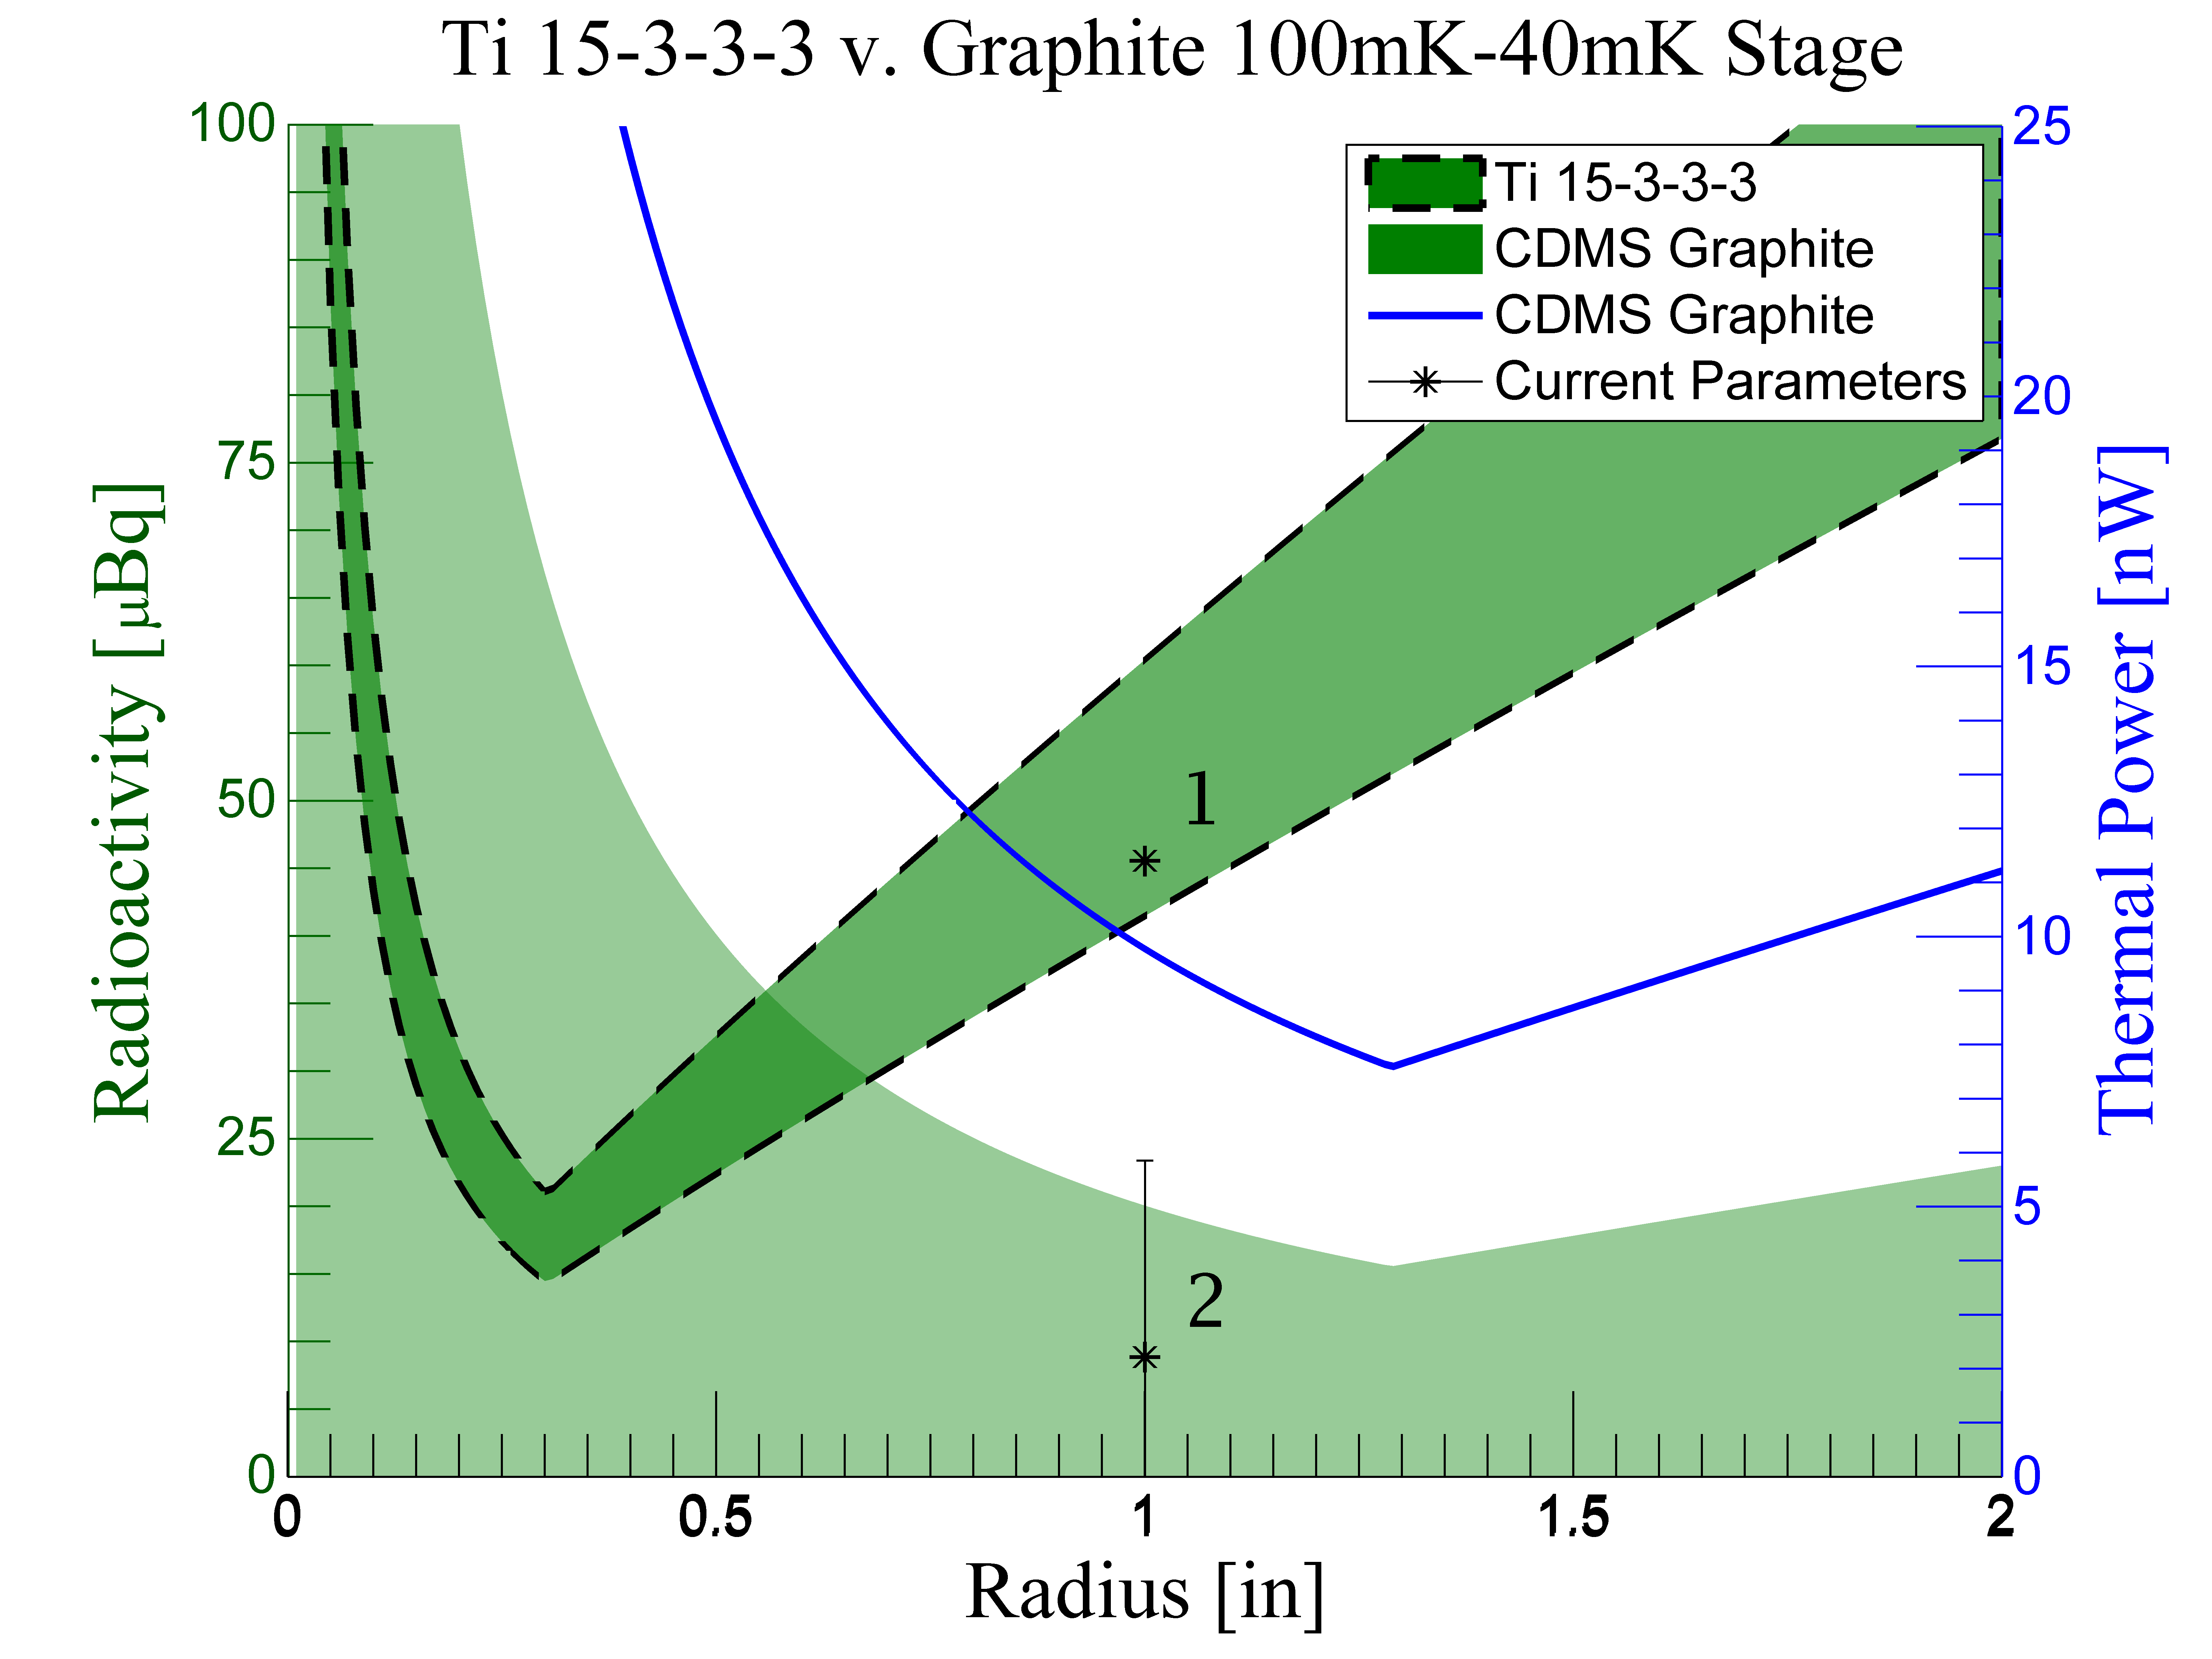
\includegraphics[width=\textwidth]{Ti15333_Graphite_100mK40mK.png}
%\end{minipage}
%\caption{Radioactivity and Thermal Power for varying dimensions. The green shaded regions represent the uncertainty in radioactivity given in table 2. The regions bounded by black
%dashed lines are those of the candidate materials. Point 1 gives current graphite heat load, while point 2 (including error bars) gives current graphite radioactivity.}
%\end{figure}

It is obvious that the candidate materials offer significant improvement over the current UF-4S Graphite. The heat load improvement per stage is examined below. For simplicity,
the values along the optimum lines have been used.

\smallskip

\large{\underline{5K -1K}}

At a radius of 0.4 inches, the power from Vespel SP-1 is 50$\mu$W. This is 1/6 the current heat load. Assuming the same thermal conductivity for Vespel SCP-5000, this number could
be reduced to near 35$\mu$W for more than an 800\% reduction in heat load.

\smallskip

\underline{{\large 1K-100mK}}

Vespel SP-1 could reduce the heat load to 1.3$\mu$W from 3.4$\mu$W, 2.6 times less than the current heat load. Vespel SCP-5000 could offer an additional 30\% improvement over SP-1.

\smallskip

\underline{{\large 100mK-40mK}}

With no data yet in this range for Ti 15-3-3-3 we cannot know the improvement, but at the optimum value, cross-section is reduced by nearly a factor of 20. Given that the thermal
conductivity of Ti 15-3-3-3 is almost certainly lower at this stage than UF-4S Graphite, a significant improvement is expected.

\bigskip

For each stage, the candidate materials not only offer a significant reduction in thermal power, but remain well within acceptable limits for radioactivity.

It should be noted that the optimized values would almost certainly result in a failure load of less than 145lbs. Given the error for the predicted Graphite failure, the actual
would be around 20-30\% lower. Even so, our failure load would still be near 100lbs. If it is decided that this is too low, the material dimensions can easily be increased and
still offer more than a factor of 2 improvement for each stage.

\section{Striplines}
In addition to modifying the tower support tubes, we are examining the feasibility of replacing the NbTi vacuum coaxial cables along tower face with a parallel strip transmission
line. This transmission line must satisfy the new inductance requirements of the SQUID/Detector designs while remaining within acceptable limits for thermal power loading on the
tower stages. Critical current density, resistivity, and critical temperature ($T_{c}$) must also be evaluated for the new line.

Our consideration of a flex cable comes from:
\begin{itemize}
\item Low inductance design capability
\item Precise control over dimensions
\item Reproducibility
\item Strength, and Low Radioactivity (from Kapton substrate)
\end{itemize}

The new SQUID design will reduce the superconducting QET resistance from 0.2$\Omega$ to 0.02$\Omega$. Since the 3dB roll-off frequency corresponds to R/L for our amplifier, when we reduce R by a factor of 10, we must also reduce inductance, L, by a factor of 10 to maintain our bandwidth. The new goal for the inductance of our flex cable is 30nH over a 20 inch length, or $\approx$ 60nH/m. To determine the inductance for our parallel traces we used the following formula used by basic inductance calculators:

$$ L \approx \frac{\mu_{0}\mu_{r}h}{w} \ \ (h > t , w >> h)$$

$\mu_{0}$ = the magnetic constant (4$\pi \cdot 10^{-7}$)\\
$\mu_{r}$ = relative permeability of Kapton (assumed to be 1)\\
t = thickness of trace \\
h = center-to-center separation of traces \\
w = width of the trace \\

Sonnet EM modeling software will be used to provide more detailed inductance modeling as well as to measure electrical cross-talk.

\subsection{NbTi Trace}

We have ordered Nb47Ti(53\% Nb, 47\% Ti by weight) which was rolled by Virginia Fine Metal. The foil is 4" x 10" and 0.002" thick. The same Nb47Ti has already been successfully etched so it can now be made into a preliminary parallel strip transmission line for testing.

\begin{table}[ht]
\centering
\begin{threeparttable}
{\footnotesize\rm\begin{tabular}{l|rrrrrr}
  \multicolumn{7}{l}{{\large Thermal Loading in Tower Stages for Current 8 Pair Design, 6 Face Tower}}\\
\toprule
 {\normalsize Material} & 4.2K-600mK & 600mK-50mK & 50mK - 10mK & 5K-1K\tnote{*} & 1K-100mK\tnote{*} & 100mK-40mK\tnote{*} \\
  &P($\mu$W)&P(nW)&P(nW)&P($\mu$W)& P(nW) & P(nW) \\ \hline\hline
  Ti15333 @ 0.0005" & - & 658.5 & 4.41 & - & 1997 & 15.44 \\
  Ti15333 @ 0.001" & - & 807.4 & 5.03 & - & 2670 & 17.60 \\
  Nb-47Ti @ 0.001" & 108.4 & 879.95 & 5.14  & 170.74 & 2767 & 18.42 \\
  Graphite Tube & 202 & 950 & 2.2 & 309 & 3400 & 11.4 \\
  Current Vacuum Coax's & 0.762 & \multicolumn{2}{r}{3.60} & 1.28 & \multicolumn{2}{r}{16.68} \\
\bottomrule
\end{tabular}
\begin{tablenotes}
   \item[*]{Thermal stability calculations provided to account for non-ideal fridge temperatures}
\end{tablenotes}}
\caption{Calculated power conducted between individual tower stages for 30nH inductance. Graphite numbers based on current support tube lengths: 4.2K-600mK stage - 0.949in; 600mK-50mK
stage - 1.572in; 50mK-10mK stage - 1.334in. Transmission line calculations used inter-stage lengths of: 4.2K-600mK - 0.688in; 600mK-50mK - 0.789in; 50mK-10mK - 0.740in. Vacuum coax
calculations used: 4.2K-600mK - 1.339in; 600mK-10mK - 0.83in. }
\end{threeparttable}
\end{table}

\subsection{Ti 15-3-3-3 Trace}
Ti 15-3-3-3 is another option as a trace material. Its relevant properties are discussed below.
\begin{itemize}
\item Thermal Conductivity: This alloy offers a lower thermal conductivity than NbTi at all stages.
\item Critical Current Density: MUST EXPERIMENTALLY DETERMINE
\item Superconducting Transition Temperature: 3.89K
\item Resistivity: MUST EXPERIMENTALLY DETERMINE
\end{itemize}

Due to it's very low transition temperature, it is not an option at the 4K to 600mK transition. If the SQUIDS are placed at the 600mK stage, Ti 15-3-3-3 is an ideal choice as a trace from 600mK down to the 10mK base.

To roll Ti 15-3-3-3 we have contacted Ulbrich, a company which could provide us with a foil as thin as 0.5 mil. The cost for even 1 mil, however, is \$1010/lb with a minimum of 10 lbs, so it will be expensive. Another possible company is called Arnold Rolled Products. They carry Ti 15-3-3-3 sheet in stock and could roll to 0.5 mil.

\bigskip

\subsection{New 50mK Stage (or 100mK for Non-Ideal) Heatsink}
 The current tower design has an internal heat sink for the 50mK stage. The only external components of this stage on the tower face are two connectors for thermally connecting
the tower support tubes to the fridge. This new transmission line design, while easily adjustable to meet inductance requirements, is much more thermally conductive; therefore,
to implement this new design, I propose adding an additional external component for heatsinking the transmission line to the 50mK fridge stage. The need for an external 50mK
heatsink can be seen in Table 5. We have used a best case transmission line design: 0.5 mil Ti 15-3-3-3 designed for 50nH/20". This is compared to the current NbTi vacuum coax's and graphite tower support tubes. The power shown is per tower with the current 6-sided design.

\bigskip

\begin{table}
\centering
\begin{threeparttable}
\begin{tabular}{l|r}
\multicolumn{2}{c}{Power Loaded to Base (40mK) [nW]}\\\toprule
Ti15333 & 1442 \\\midrule
Current Vacuum Coax's & 16.68\\\midrule
Graphite Tube & 11.4 \\ \bottomrule
\end{tabular}
\end{threeparttable}
\caption{Power load on tower base. For simplicity, only the non-ideal temperature calculations are provided.}
\end{table}

\bigskip
Assuming the internal 50mK stage heatsink can be brought out, we can have  a thermally competitive design for the parallel strip transmission line. Table 4 compares an NbTi line, Ti 15-3-3-3 line, current coax's, and the Graphite tube. NbTi only goes to 1 mil, as it cannot be rolled thinner. Ti 15-3-3-3 is presented in 0.5 mil and 1 mil, as it can be produced in 0.5 mil, but it will be expensive.

\section{Availability}
\subsection{Vespel SP-1/Vespel SCP-5000}

Vespel SP-1 and SCP-5000 are both readily available from DuPont through the certified distributor Curbell Plastics.

As a warning, an employee from Curbell Plastics notified us that another company, Pro Plastics, sells a counterfeit material under the name of Vespel.

\subsection{Carbone UF-4S}

This is the grade currently used in the towers as a support tube. Through recent contact with Mersen (the new owner of Carbone of America) we have found that this grade is still produced and readily available.

\subsection{Ti 15-3-3-3/Ti 21s}

Ti 15-3-3-3 is not available in anything except sheet form in the United States. Chinese companies, however, have Ti 15-3-3-3 available as wire, sheet, and rod. Two possible
companies are YR Titanium and ReTi Metal. Two rods have been ordered from ReTi Metal.

Ti 21s is another metastable-$\beta$ alloy with similar properties to Ti 15-3-3-3. Tests will be conducted to determine its suitability.

\subsection{Stripline Companies}
\subsubsection{Rolling}
\begin{itemize}
\item Hamilton Materials
\item Virginia Fine Metals
\item Arnold Rolled Products
\end{itemize}

\subsubsection{Transmission Line Fabrication}
\begin{itemize}
\item Luxel
\item Tech-Etch
\end{itemize}

\chapter{Design of Low Conductivity Electronics for the Detector Tower}

The next generation of the CDMS experiment -- SuperCDMS SNOLab -- features substantial redesigns for the detectors/readout electronics. These alterations include using more phonon read-out channels for the detectors, adding high-electron-mobility transistors (HEMTs) as low-noise amplifiers for the charge read-out, and new SQUIDs. These alterations will require the development of new wiring for phonon readout, charge readout, and for the 300K - 4K striplines. These lines have their own specific set of considerations for development which will dictate their design. The phonon readout design will require low a thermal conductance, low inductance, flexible stripline which meets various resistance requirements, the charge readout must be low noise and low thermal conductance, and the 300K - 4K striplines must meet thermal conductance and resistance requirements. The following sections will examine these requirements, and discuss the design options which satisfy them.

\section{Phonon Readout Cable}

For SuperCDMS SNOLab, the phonon readout lines will move from a vacuum coax design, to a flexible transmission line. The primary impetus for this is that the new SQUIDs will require a transmission line with a much lower inductance between the detectors and the SQUIDs. From here, we have the secondary design considerations of low thermal conductance and resistance limits. Low thermal conductance is especially important for the new phonon readout line for two reasons: First, the flexible transmission line has a substrate, which includes much more material than a vacuum coax, so has more potential for high heat loads. Second, we are increasing the phonon channels per detector from 4 to 6, so there will be increased trace numbers (which increases transmission line width). Last, we must meet two resistance requirements. The first requires superconducting traces between the detectors and the SQUIDs, while the second sets an as-of-yet undefined resistance limit on the traces from the SQUIDs to the HEMTs.

\subsection{Thermal Conductivity of Constituent Materials}

Due to the increase in expected heat load associated with switching to a flexible phonon readout transmission line, the thermal conductivities of the cable materials is a large factor in their selection. The cable will consist of a polyimide substrate, a metallic trace, and some form of adhesive/epoxy (depending on the fabrication). The thermal conductivities of these are examined below.

\subsubsection{Kapton}

Though there are other options for substrate materials, Kapton is the default for cryogenic cabling, as it is known to have low thermal conductivity, as well as high radiopurity. It is often the primary substrate material offered by fabrication companies, therefore we would like to characterize its thermal conductivity. In particular, we are interested in Kapton HN data, as it is the type used by Tech-Etch -- a cryogenic cable fabrication company which will likely make the phonon cable. The thermal conductivity for Kapton HN samples, as well as other types, are shown Figure 4.1. The power law fit of these thermal conductivities in the range of interest is presented in Table 4.1; some of these were given in the references, and some are fits to graphical data presented in references. The thermal conductivity data from M. Barucci \cite{bar} was chosen to model heat loads for the cable in the following sections. This thermal conductivity is markedly higher than most of the other data. This is likely due to the direction of measurement along the sample; Barucci measures the thermal conductivity along a strip of Kapton, while other authors use a laminate of Kapton strips and measure through the thickness of the laminate (perpendicular to the Kapton strip direction). Unless the Kapton is isotropic, this would result in a different measured thermal conductivity.

\begin{figure}[h]
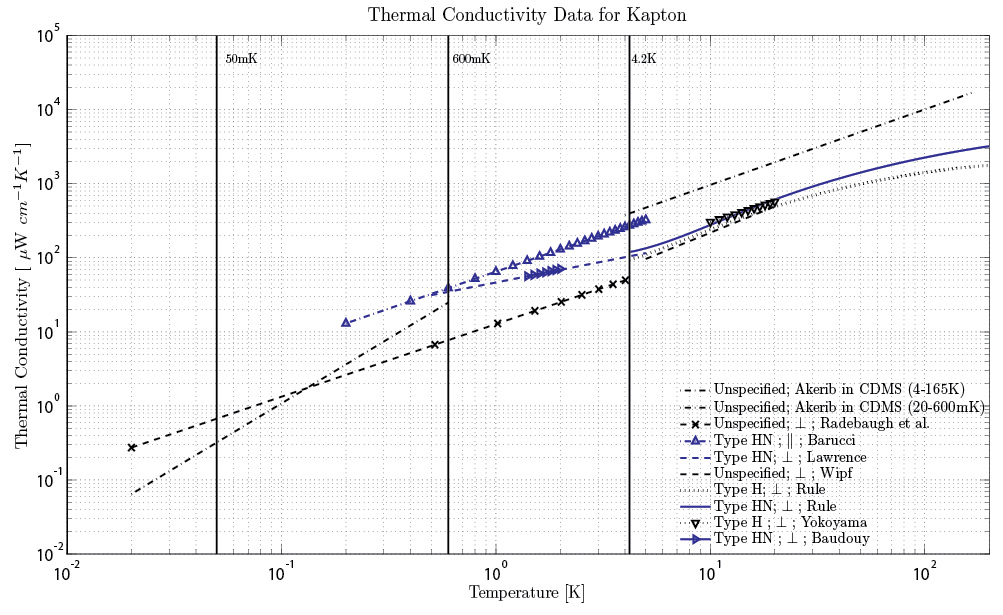
\includegraphics[width = .9\textwidth]{Kapton_var.png}
\caption{Compiled data for the thermal conductivity of Kapton films. The type is specified in the legend, as well as whether measurements were performed parallel or perpendicular to the Kapton surface. The direction of Kapton measurement is not stated when unknown. Data are from Radebaugh \cite{rad73}, Barucci \cite{bar}, Lawrence \cite{law}, Wipf \cite{wip}, Rule \cite{Rule1996}, Yokoyama \cite{yok}, Baudouy \cite{Baudouy2003}, and Akerib \cite{Akerib}. }
\end{figure}

\begin{table}[h]
\centering
\begin{threeparttable}
\begin{tabular}{llclr}
\toprule
Author & Type & Dir. of Measurement & k(T) [ $\mu$W/cm-K] & Temperature Range [K]\\
\midrule
Wipf \cite{wip} & Unspecified & $\perp$ & $14.51 \cdot T^{1.177}$ & 5 - 20 \\
Lawrence \cite{law} & HN & $\perp$ & $46.38 \cdot T^{0.568}$ & 0.5 - 5 \\
Rule \cite{Rule1996} & HN & $\perp$ & $24.7 \cdot T^{1.043}$ & 4.2 - 10 \\
Rule \cite{Rule1996} & H & $\perp$ & $18.2 \cdot T^{1.121}$ & 4.2 - 10 \\
Barucci \cite{bar} & HN & $\parallel$ & $65 \cdot T$ & 0.2 - 5 \\
Radebaugh \cite{rad73} & Unspecified & $\perp$ & $12.73 \cdot T^{0.982}$ & 0.02 - 4 \\
Akerib \cite{Akerib} & Unspecified & ? & $60.7 \cdot T^{1.75}$ & 0.02 - 0.6  \\
Akerib \cite{Akerib}& Unspecified & ? & $92 \cdot T^{1.02}$ & 4 - 165 \\
Yokoyama \cite{yok} & H & $\perp$ & $36.87 \cdot 10^{0.9154}$ & 10 - 300 \\
Baudouy \cite{Baudouy2003} & HN & $\perp$ & $22.8 + 24.0 \cdot T$ & 1.4 - 2 \\
\bottomrule
\end{tabular}
\caption{Power law fits for thermal conductivity of Kapton in range of interest. The direction of measurement specifies whether thermal conductivity was taken parallel or transverse to the surface of a Kapton strip.}
\end{threeparttable}
\end{table}


\subsection{Thermal Conductivities of Trace Materials}

The thermal budget is very tight for the phonon line, as the thermal conductance is already expected to be much higher than for the current vacuum coax design, so thermal conductivity is a large consideration for trace material selection. Figure 4.2 presents the thermal conductivities of candidate materials; in the cases where multiple thermal conductivities are given for each material, we give rough upper and lower limits on thermal conductivity (from a literature search and from our own testing).

\begin{figure}[h]
\centering
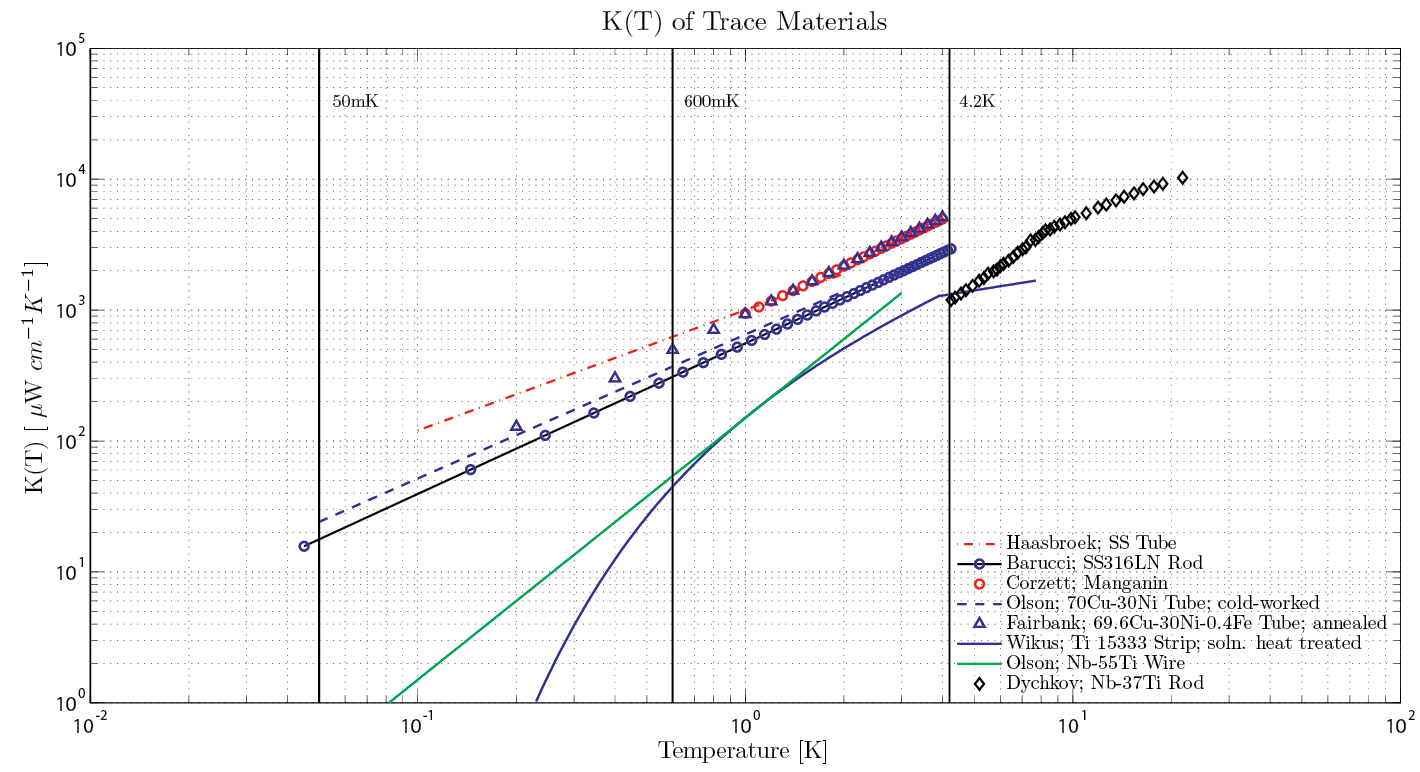
\includegraphics[width = .8\textwidth]{Trace_material_k.png}
\caption{Thermal conductivities for trace materials. High and low values were taken from the literature when a significant variation was present among data. Data from: Haasbroek \cite{has}, Barucci \cite{Barucci2008}, Corzett \cite{cor}, Olson \cite{ols}, Fairbank \cite{fair}, Wikus \cite{wik}, Dyachkov \cite{dya}.}
\end{figure}


\subsection{Resistivities of Trace Materials}
Since Ti15-3 has a transition temperature of 3.9K (as measured at MIT), it will not be in a superconducting state throughout the 4.2K - 600mK span. However, as long as the resistivity remains low, it can still be used. Table 2 presents the resistivity as compared to other possible trace materials.

\begin{table}[h]
\centering
\begin{threeparttable}
\begin{tabular}{l|c|c|c|c}
Alloy & \multicolumn{3}{c}{Resistivity in $\mu$ $\Omega$ $cm$} \\\toprule
 & 300K & 273K & 10K & 4.2K \\\midrule
70Cu-30Ni & - & 38.4 & - & 36.4 \\
Constantan & 49.1 & - & 46.1 & - \\
Manganin (4\%Ni) & 47.6 & - & 41.9 & - \\
Ti15-3 & 146 & - & - & 173 \\
SS316 & - & 76.5 & - & 55.3 \\
50Nb-50Ti & 76.7 & - & 54 & 0 \\
\end{tabular}
\end{threeparttable}
\caption{Resistivities of possible trace materials.}
\end{table}

Though the resistivity of Ti15-3 is higher than other candidate materials, if we consider a trace 10 mils wide and 1 mil thick, we get a resistance of
$$
\frac{R}{Length} = \frac{173 \cdot 10^{-6} \Omega cm}{6.45 \cdot 10^{-5} cm^{2}} = 2.68 \Omega / cm
$$

\subsection{Phonon Transmission Line Dimensions}

The new proposed dimensions for the phonon transmission line are shown below. The total widths of the lines (as given below) are larger than previously thought, which may alter design considerations. The trace separation is 10 mil between every trace, regardless of width. Though this places adjacent traces near one another, by alternating trace types as shown in Figures 3,4, and 5, we can increase the spacing between the lines whose cross-talk we are concerned with.

\begin{itemize}
\item 4.2K to 600mK
    \begin{itemize}
    \item 4.2K-600mK cable length = 9.24cm
    \item Trace width = 10 mil
    \item Total traces = $2\cdot12$ QET Bias Resistor + $2\cdot12$ SQUID Bias + $2\cdot12$ SQUID Feedback + $2\cdot6$ LED + $2\cdot4$ Charge Readout Bias + $2\cdot4$ Charge Feedback = 100 Traces
    \item Horizontal trace separation = 10 mil
    \item Trace thickness = 0.8 mil
    \item Total line width = 1.01 inches
    \item Total trace cross-section = 0.0052 $cm^2$
    \item Total Kapton cross-section = 0.0098 $cm^2$
    \item Total adhesive cross-section = 0.0130 $cm^2$
    \end{itemize}
\item 600mK to 50mK
    \begin{itemize}
    \item 600mK-50mK cable length = 5.04cm
    \item Trace width:
        \begin{itemize}
        \item QET Signal = 40 mil
        \item QET Bias Resistor, LED line, Thermometry line, Charge readout = 10 mil
        \end{itemize}
    \item Total traces = $2\cdot12$ QET Signal + $2\cdot12$ QET Bias Resistor + $2\cdot6$ LED + $2\cdot4$ Charge Readout Bias + $2\cdot4$ Charge Feedback = 76 Traces
    \item Horizontal trace separation = 10 mil
    \item Trace thickness = 0.8 mil
    \item Total line width = 1.13 inches
    \item Total trace cross-section = 0.0076 $cm^2$
    \item Total Kapton cross-section = 0.0109 $cm^2$
    \item Total adhesive cross-section = 0.0146 $cm^2$
    \end{itemize}
\end{itemize}

\newpage

\begin{figure}[h]
\centering
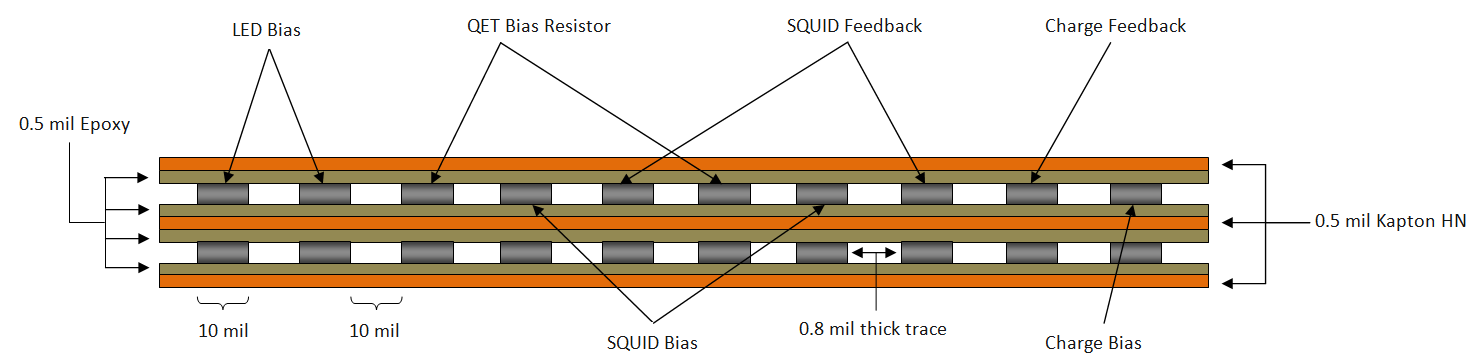
\includegraphics[width = .9\textwidth]{4K_600mK_diagram.png}
\caption{Cross-section for 4K-600mK phonon transmission line showing 20 of the 100 traces.}
\end{figure}
~\\
~\\
\begin{figure}[h]
\centering
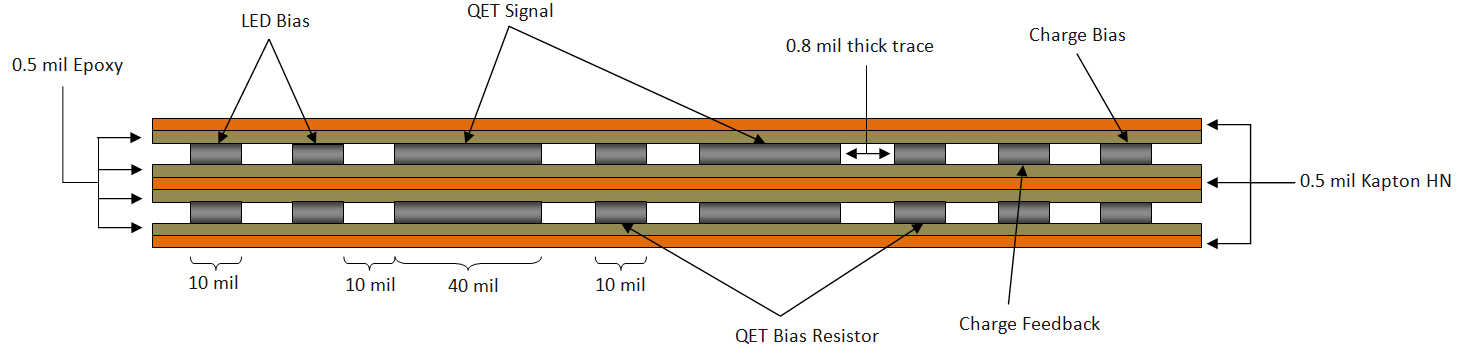
\includegraphics[width = .9\textwidth]{600mK_50mK_diagram.png}
\caption{Cross-section for the 600mK-50mK section of the phonon transmission line showing 16 of the 76 traces.}
\end{figure}
~\\
~\\
\begin{figure}[h]
\centering
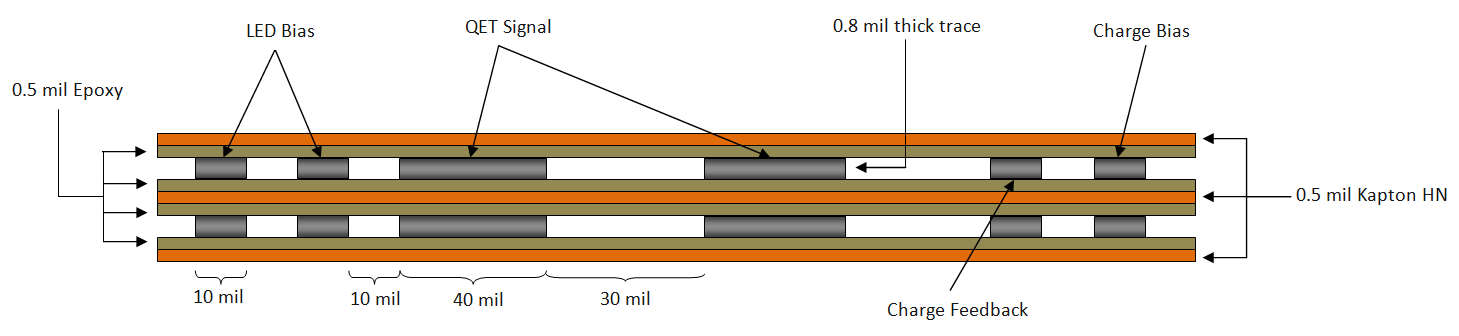
\includegraphics[width = .9\textwidth]{50mK_10mK_diagram.png}
\caption{Cross-section for the 50mK-10mK section of the phonon transmission line showing 12 of the 52 traces.}
\end{figure}

\newpage

\begin{itemize}
\item 50mK to 10mK
    \begin{itemize}
    \item 50mK-10mK cable length = 3.25cm
    \item Trace width:
        \begin{itemize}
        \item QET Signal = 40 mil
        \item LED line, Thermometry line, Charge readout = 10 mil
        \end{itemize}
    \item Total traces = $2\cdot12$ QET Signal + $2\cdot6$ LED + $2\cdot4$ Charge Readout Bias + $2\cdot4$ Charge Feedback = 52 Traces
    \item Horizontal trace separation = 30 mil between QET ; 10 mil between all else
    \item Trace thickness = 0.8 mil
    \item Total line width = 1.13 inches
    \item Total trace cross-section = 0.0064 $cm^2$
    \item Total Kapton cross-section = 0.0109 $cm^2$
    \item Total adhesive cross-section = 0.0146 $cm^2$
    \end{itemize}
\end{itemize}

\subsection{Phonon Transmission Line Heat Load}

The heat loads for the Phonon line using different trace materials are shown below \footnotemark. As you can see, the heat load from the traces is significant, especially for the 4.2K-600mK span.
The 50mK-10mK span assumes placement of a heat sink at the detector end of the tower (before the copper tube which holds the detector housings) which shortens the 50mK-10mK cable length to only 3.25cm. If we were to create a heat sink closer to the detectors, this could be significantly reduced.

\begin{table}[h]
\begin{threeparttable}
\begin{tabular}{rrrr|rrr}
\toprule
 & \multicolumn{6}{c}{Heat Load for 48 Towers in $\mu$W} \\
  & 5K-1K & 1K-100mK & 100mK-40mK & 4.2K-600mK & 600mK-50mK & 50mK-10mK \\
 \cmidrule(r){2-7}
   Ti15-3 \cite{wik} & 590.6 & 20.20 & $1.0\cdot10^{-4}$ & 412.5 & 2.93 & $1.1 \cdot 10^{-6}$ \\
   45Nb-Ti \cite{ols} & 1047 & 22.89 & 0.0279 & 623.9 & 4.95 & 0.0037 \\
   Manganin (2\%Ni) \cite{Peroni1999} & 2476 & 192.9 & 1.321 & 1707 & 62.19 & 0.317 \\
   SS316 \cite{lou} \cite{Barucci2008} & 1347 - 1846  & 117.7 - 235.8 & 0.938 - 3.087 & 941.1 - 1351 & 39.33 - 88.76 & 0.238 - 0.9405 \\
   70Cu-30Ni \cite{pob} \cite{ols} & 1483 - 2480 & 140.7 - 190 & 1.25 - 1.273 & 1047 - 1706 & 48.26 - 60.94 & 0.303 - 0.330 \\
   Al5056 \cite{Coccia1983} & 3.98E+5 & 2273 & .4225 & 2.05E+5 & 321.1 & 0.031 \\
   Kapton \cite{bar} & 237.6 & 20.11 & 0.265 & 171.1 & 7.26 & 0.076 \\
   Epoxy Adhesive &&&&&& \\
   \multicolumn{2}{c}{\bf{Total Phonon Line}} & & & & & \\
   with Ti15-3 & 828.3 & 40.31 & 0.265 & 583.6 & 10.19 & 0.076 \\
   with 45Nb-Ti & 1285 & 43.00 & 0.292 & 795 & 12.21 & 0.0793 \\
   with Manganin & 2714 & 213 & 1.585 & 1878 & 69.45 & 0.3925 \\
   with SS316 & 1584 - 2083 & 137.8 - 255.9 & 1.203 - 3.351 & 1112 - 1522 & 46.59 - 96.02 & 0.314 - 1.016 \\
   with 70Cu-30Ni & 1721 - 2717 & 160.8 - 210.1 & 1.515 - 1.537 & 1218 - 1877 & 55.52 - 68.2 & 0.3787 - 0.406 \\
   with Al5056 & 3.99E+5 & 2293 & 0.687 & 2.05E+5 & 328.1 & .106 \\
  \bottomrule
\end{tabular}
\end{threeparttable}
\caption{Heat loads for constituents of the phonon cable as well as the total cable heat load for various materials for a total of 48 towers. Assumes all trace thicknesses are 0.84 mils. The large heat load at the 50mK-10mK span for the phonon cable is due to short cable length (3.25cm) created by placing a heat sink at the bottom of the tower.}
\end{table}

\footnotetext{Constantan (55Cu-45Ni) was considered as an alternative to Cupro-Nickel, due to its lower Copper content. However, it was found \cite{tou} to have a higher thermal conductivity than 70Cu-30Ni.}

\newpage
\subsection{Sonnet Modeling for Phonon Line}
Between the SQUIDS and our detectors, we have set an inductance limit of roughly 30nH between signal/return lines. To ensure that our cable would meet this requirement, Sonnet modeling software was used to simulate the line with 40mil wide, 0.8mil thick traces at a center-to-center separation of 2.3mil. This yields:
$$
L = 22.4\frac{nH}{20"}
$$
as well as,
$$
C = 471\frac{pF}{20"}
$$
for capacitance between the lines.

\section{Charge Readout Lines}

The form of the future charge readout lines is still under debate. Since noise is only a concern on the gate wires, the charge feedback and bias pairs can be integrated into the flexible parallel-trace transmission line design. The 4 remaining gate wires have a few available options. The simplest option would be for the lines to remain vacuum coaxes. The next option involves a flexible coaxial cable produced by AXON' The last option would be to make our own cable with low noise properties.

If we keep the vacuum coaxes, we will alter the design slightly to allow removal of the coaxes from the tower. This would involve a type of carbon fiber rod supported frame to which the wires are mounted, as depicted in Figure 6. Though this could be a low heat load design, it is the least convenient option. Heat loads are presented in Table 4. The wires would be the same 1.2 mil diameter NbTi lines currently used in our towers, however would have an additional heat sink at the newly available externalized 50mK stage on the next generation tower design. We see that the heat loads for this option are rather large, due to the carbon fiber rods. While the calculations have assumed a 40mil rod thickness, our supplier for rods also has 33mil, 30mil, 20mil, and 10mil diameter rod options, which could reduce heat loads.

The next option involves a coaxial cable from AXON' \footnotemark.
\footnotetext{Another company, Texcal, was considered, as they also produce low-noise cabling. Unfortunately, their cables use silver-plated copper conductors, whose thermal conductivity far exceeds what is acceptable for our purposes.}
This cable uses Constantan as a conductor material, PTFE for a housing, and Celloflan dielectric (porous PTFE); The cable's cross-section is shown in Figure 6. A thin graphite coating on the outside of the Celloflan dielectric prevents static charge build-up on the insulator -- our main source of noise in the gate wires. The suitability of this option depends on expected heat loads from the cable. These are shown in Table 4. The calculations use Cupro-Nickel (70Cu-30Ni) thermal conductivity in place of Constantan \footnotemark, as well as simple PTFE in place of Celloflan. The high expected heat loads from this cable will likely rule it out as a candidate for replacing the vacuum coax design.

\footnotetext{It was found that the actual thermal conductivity of Constantan is slightly higher than Cupro-Nickel, but is close enough for approximation purposes. If this is considered a viable option, more accurate calculations will be done.}
Another option is to simply alter a cable to have low-noise characteristics. This could be made possible with a flexible polyimide cable whose dielectric has undergone ion implantation to increase the conductivity to near that of graphite \footnotemark. This would serve the same function as the graphite layer in the AXON' coaxial cable -- preventing static charge build-up. Heat loads for this option are not presented, as the potential form of these cables is as-of-yet unknown.

\footnotetext{See, for instance, \cite{Chen2009}}

\begin{figure}[h]
$\vcenter{\hbox{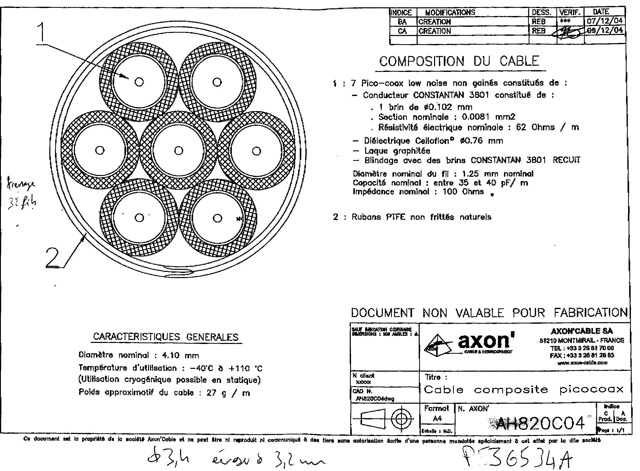
\includegraphics[width = .5\textwidth]{Edelweiss_cable.jpeg}}}$
$\vcenter{\hbox{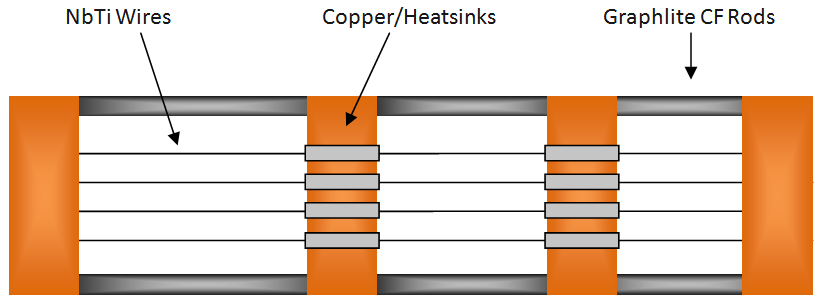
\includegraphics[width = .5\textwidth]{Charge_vacuum_design.png}}}$
\caption{Two possible designs for future charge gate wires. Left is the specially made AXON' cable (to have a Conastantan conductor). Right shows the basic structure of a removable vacuum coax design with copper heatsink connections supported by carbon fiber rods.}
\end{figure}

\subsection{Charge Readout Heat Loads}

The total charge readout line heat load contribution for a 12 tower experiment is presented below in Table 4. These calculations assume 4 gate wires per detector, so 288 wires for 12 towers (or 288 coaxes in the case of the AXON' cable).

\begin{table}[h]
\begin{threeparttable}
\begin{tabular}{rrrr|rrr}
\toprule
 & \multicolumn{6}{c}{Charge Coax Heat Loads for 12 Towers in $\mu$W} \\
  & 5K-1K & 1K-100mK & 100mK-40mK & 4.2K-600mK & 600mK-50mK & 50mK-10mK \\
 \cmidrule(r){2-7}
   Vacuum Coax Design & 122.3 & 16.34 & 0.135 & 94.3 & 5.17 & 0.031 \\
   AXON' Cable & 2736 - 4439 & 261.56 - 351.22 & 3.163 - 3.221 & 1862 - 2988 & 88.59 - 110.91 & 0.768 - 0.827 \\
  \bottomrule
\end{tabular}
\end{threeparttable}
\caption{Heat loads for charge readout coaxes for 12 towers. With 50mK heat sinking, assumes cable lengths of: 4.2K - 600mK = 7.8cm ; 600mK - 50mK = 2.7cm ; 50mK - 10mK = 1.5cm. Assumes 4 lines (or coaxes) per detector, 6 detectors per tower. The vacuum coax calculations assume two 40 mil diameter rods between each stage, which constitute the frame for the removable vacuum coaxes. These dominate the heat loads ($>95\%$).}
\end{table}

\section{Wiring for 300K - 4.2K}

We must design cable to run from room temperature (300K) to the HEMTs on the tower (4.2K). This cable must meet resistance, thermal, and practical requirements. The upper limit on round trip resistance for the lines is around 200$\Omega$, while the upper limit for heat load is 500mW on 4.2K. Apart from these considerations, the cable must be thin enough to be flexible, the dimensions work-able, and the traces should be solderable\footnotemark.

To meet the heat load restrictions of the cable, a 77K heat sink will be placed along the cable. This will be located around 20" down the cable from room temperature. From here, the 77K - 4.2K length will run around 90" until the 4.2K heat sink. From here, there will be 20" to the HEMTs at the tower. 500mW is a larger heat load than we expect from any reasonably designed cable, so minimizing heat load is not the primary design consideration.

\footnotetext{OFHC Copper was considered as an option, as it is the easiest to solder and has a much smaller resistivity, but the thermal conductivity was nearly 5 orders of magnitude higher than the range of materials in Figure 7. Dimensions could not be decreased enough to produce a viable heat load.}

The resistivity of some of the candidate materials is shown in Table 2. This will set a limit on the minimum dimensions of the traces to keep below 200$\Omega$ for the lines. This, as well as the ease with which the traces can be manufactured into a cable (ability to solder to the traces, flexibility, strength, availability) is the main consideration for selection of dimensions and trace material.

\begin{SCfigure}
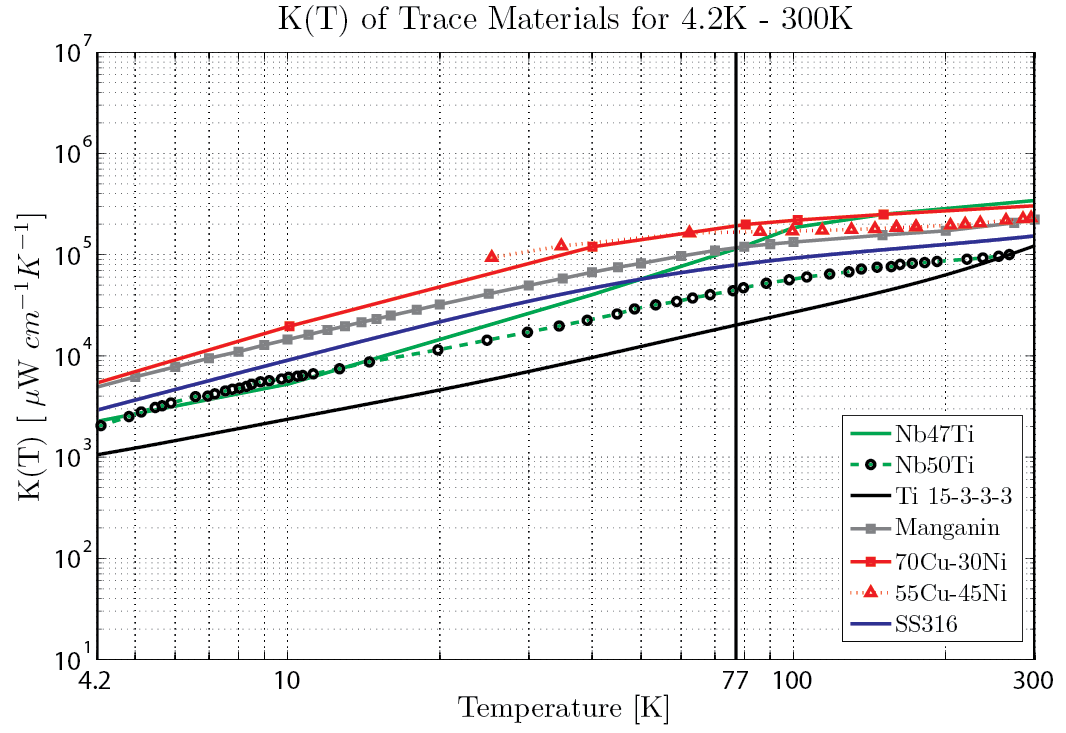
\includegraphics[width = .65\textwidth]{Trace_matl_300K.png}
\caption{Thermal conductivities of viable trace materials for a cable spanning 4.2K to 300K. References for data are: \newline Nb47Ti - Tekdata website ; Nb50Ti - Flachbart \cite{Flachbart1978} ; Ti 15333 - Wikus \cite{wik} ; Manganin (84Cu-4Ni-12Mn) - Touloukian \cite{tou} ; 70Cu-30Ni - Tekdata website ; 55Cu-45Ni - Touloukian \cite{tou} ; SS316 - NIST database.}
\end{SCfigure}

\subsection{Expected Heat Loads}

The predicted heat loads for some of the candidate materials on the 77K stage and 4.2K stage are presented in Table 5. These heat loads assume the cross-sections presented for each material in the same table. Cross-sections for each material were minimized based on each material's resistivity to produce a line resistance of 200$\Omega$. As the resistivity of each material varies with temperature, the maximum value of resistivity from Table 2 was assumed for each material across the temperature range to provide a safety buffer in resistance.

The heat loads are all relatively similar despite very different thermal conductivities, due to the different minimum cross-sections. After factoring in resistance, the advantage of Ti15-3-3-3 over 70Cu-30Ni is only a factor of 2 for power onto 4.2K, despite Ti15-3-3-3 being about a factor of ten better in thermal conductivity.

Considering the difficulty in fabricating a cable out of Ti15-3-3-3, and the large dimensions that would be required for a Ti15-3-3-3 trace (30 mil wide traces would still have to be 7.5 mils thick) it is not the best option. Instead, Manganin or 70Cu-30Ni are recommended.

\begin{table}[h]
\centering
\begin{threeparttable}
\begin{tabular}{l|ccc}
\toprule
Material & $A_{min}$ [$cm^2$] & Power to 77K [$\mu W$] & Power to 4.2K [$\mu W$] \\
\midrule
70Cu-30Ni & 1.2680E-4 & 1.301E+7 & 3.802E+5 \\
Ti15-3-3-3 & 5.7125E-4 & 1.374E+7 & 1.605E+5 \\
Manganin (4\%Ni) & 1.5718E-4 & 1.0220E+7 & 2.862E+5 \\
SS316 & 2.526E-4 & 1.187E+7 & 3.180E+5 \\
\bottomrule
\end{tabular}
\end{threeparttable}
\caption{Minimum cross-sections and expected heat loads for candidate materials for a 48-tower experiment. Minimum cross-sections are calculated from the maximum resistivities of each material in Table 2 and used to calculate heat loads.  Only some of the candidate materials are presented for comparison, as heat loads are not a major concern.}
\end{table}


\section{Tower Thermal Stand-offs}
Unlike the wiring, the thermal stand-offs for the tower can be made out of a multitude of materials. Both tube and hexa-pod structures have been proposed for these materials. These candidates are evaluated based on their thermal conductivity and their strength (which allows us to decrease their cross-sectional area).

\subsection{Thermal Conductivities of Tower Materials}
In SuperCDMS, the dominant heat load came from the thermal stand-offs, so replacement materials aim for a significant improvement in thermal power conducted between stages. Figure 8 shows the candidate materials for thermal stand-offs based on radioactivity screening acceptability. Though the Graphlite rods are much higher in thermal conductivity, their strength makes them a viable material.

\begin{figure}
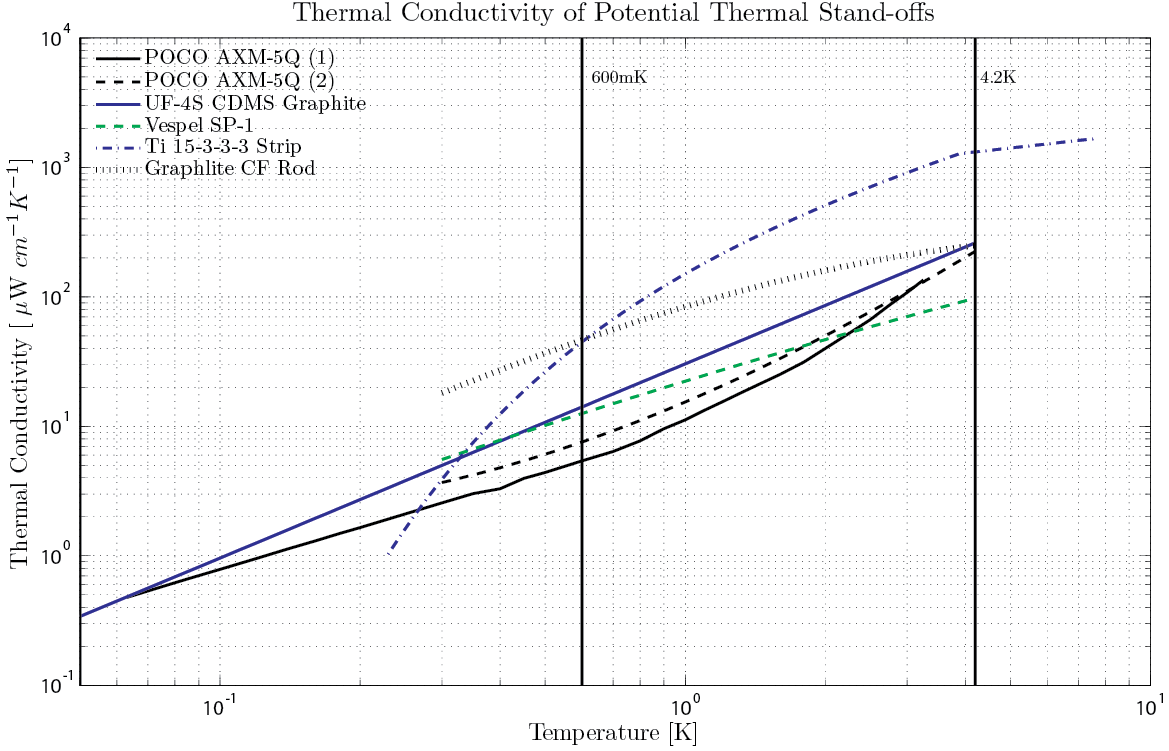
\includegraphics[width = \textwidth]{Stand_off_graph.png}
\caption{Thermal conductivities of candidate thermal standoff materials. POCO AXM-5Q (1) is from Woodcraft \cite{woo:gr} , while POCO AXM-5Q (2) was measured by Marc Runyan at Caltech \cite{run}.}
\end{figure}

\subsection{Stand-off Configurations}
There are currently two possibilities for the thermal stand-off configuration. The first is a hexapod structure, while the second is a thin walled tube.

The hexapod structure allows us to limit power loads by angling the stand-off material, which increases the effective length of the material. In addition, it limits cross-sections, as it is a very open structure. This has only been proposed for the Graplite rods so far, but could conceivably be applied to the Vespel or Ti15-3 as well.

The other materials were designed to be thin walled tubes. The dimensions of the tubes were optimized using the analytical model given in my earlier report. Using a given tube length, radius and thickness are optimized to minimize cross-section while maintaining a failure limit of 130 lbs (59 kg). This limit is in shear loading of the tower (mimicking holding the tower sideways with the detectors attached). The detectors themselves will weigh 1.4 kg apiece. With 6 detectors that is around 10 kg. We will need to figure out the equivalent load at the end of the tube to see if this results in greater than 130 lbs.

\subsection{Stand-off Heat Loads}

The stand-off lengths used to calculate heat loads were chosen to be: 4.2K-600mK = 1.68 inches ; 600mK-50mK = 1.65 inches ; 50mK-10mK = 1.30 inches. These can easily be adjusted depending on heat load constraints. The heat loads for materials of various dimensions were calculated for each stage. At each stage, the heat load for CF Graphlite rods was calculated, based on dimensions suggested by Marc Runyan. In addition, several thin-wall tube candidates are presented. The heat load for optimized dimensions are given, as well as "safer" dimensions (larger  radius and/or thickness).

\begin{table}[h]
\begin{small}
\begin{threeparttable}
\begin{tabular}{lrrrrl}
  \multicolumn{5}{l}{{\Large 4.2K - 600mK: Thermal Stand-off Heat Loads in $\mu$W, 12 Towers}} \\
\toprule
\bf{{\large Material}}& \multicolumn{2}{c}{145lb. Failure} & \multicolumn{2}{c}{290lb. Failure} & Ref.\\
\cmidrule(r){2-5}
& 5K - 1K & 4.2K - 600mK & 5K - 1K & 4.2K - 600mK & \\
Current CDMS Graphite; $(2"\oslash,0.028")$  & 3708 & 2424 & 3708 & 2424 & \cite{lem}\\
6 Graphlite CF Rods; ($0.08" \oslash$ @ $45^{o}$) & 308.4 & 238.8 & 308.4 & 238.8 & \cite{run}\\
Vespel SCP-5000; $(0.74"\oslash,0.024")|(0.94"\oslash,0.030")$ & 282.6\tnote{\dag} & 203.5\tnote{\dag} & 448.4\tnote{\dag} & 322.9\tnote{\dag} & \cite{run}\\
Vespel SP-1; $(.96"\oslash,0.027")|(1.2"\oslash,0.0347")$ & 412.7 & 297.1 & 662.6 & 477.2 & \cite{run}\\
POCO-AXM 5Q; $(1.86"\oslash,0.013")|(2.28"\oslash,0.0172")$ & (900,721) & (446,425) & (1467,1175) & (726,693) & \cite{woo:gr},\cite{run}\\
Ti 15-3-3-3 $(0.66"\oslash,0.0055")|(0.82"\oslash,0.0072")$ & 720.5 & 503.2 & 1168.3 & 816.0 & \cite{wik}\\
\bottomrule
\end{tabular}
\begin{tablenotes}
\item[\dag] Note that the integrated thermal conductivity of Vespel SP-1 was used as a proxy for
    SCP-5000.
\end{tablenotes}
\end{threeparttable}
\caption{Heat loads for 4.2K-600mK stage including non-ideal fridge temperatures. Structures designed for both 145lb. and 290lb. failure limits. Dimensions are given in (diameter, thickness) pairs for tubes. The left and right set correspond to 145lb. and 290lb. failure limits respectively. The CF Graphlite supports are rods with the given dimensions. Varying POCO heat loads come from the two referenced data. Stage length is 1.68 inches.}
\end{small}
\end{table}

\begin{table}[h]
\begin{small}
\begin{threeparttable}
\begin{tabular}{lrrrr}
  \multicolumn{5}{l}{{\Large 600mK - 50mK: Thermal Stand-off Heat Loads in $\mu$W, 12 Towers}} \\
\toprule
\bf{{\large Material}}& \multicolumn{2}{c}{145lb. Failure} & \multicolumn{2}{c}{290lb. Failure} \\
\cmidrule(r){2-5}
& 1K - 100mK & 600mK - 50mK & 1K - 100mK & 600mK - 50mK \\
Current CDMS Graphite; $(2"\oslash,0.028")$  & 40.8 & 11.4 & 40.8 & 11.4\\
6 Graphlite CF Rods; ($0.08" \oslash$ @ $45^{o}$) & 15.0 & 4.8 & 15.0 & 4.8 \\
Vespel SCP-5000; $(0.74"\oslash,0.024")|(0.94"\oslash,0.030")$ & 10.5\tnote{\dag} & 3.5\tnote{\dag} & 16.8\tnote{\dag} & 5.6\tnote{\dag} \\
Vespel SP-1; $(.96"\oslash,.027")|(1.18"\oslash,0.035")$ & 15.4 & 5.2 & 24.8 & 8.3 \\
POCO-AXM 5Q; $(1.84"\oslash,.013")|(2.26"\oslash,0.0172")$ & (6.6,9.1) & (2.1,3.0) & (10.7,14.9) & (3.4,4.8) \\
Ti 15-3-3-3 $(0.66"\oslash,.0054")|(0.82"\oslash,0.0071")$ & 9.1\tnote{\S} & 1.3\tnote{\S} & 14.9\tnote{\S} & 2.2\tnote{\S} \\
\bottomrule
\end{tabular}
\begin{tablenotes}
\item[\dag] Note that the integrated thermal conductivity of Vespel SP-1 was used as a proxy for SCP-5000.
\end{tablenotes}
\end{threeparttable}
\caption{Heat loads for 600mK - 50mK stage including non-ideal fridge temperatures. Structures designed for both 145lb. and 290lb. failure limits. Dimensions are given in (diameter, thickness) pairs for tubes. The left and right set correspond to 145lb. and 290lb. failure limits respectively. The CF Graphlite supports are rods with the given dimensions. Stage length is 1.65 inches. References for data are the same as in Table 5.}
\end{small}
\end{table}

\begin{table}[h]
\begin{small}
\begin{threeparttable}
\begin{tabular}{lrrrr}
  \multicolumn{5}{l}{{\Large 50mK - 10mK: Thermal Stand-off Heat Loads in $\mu$W, 12 Towers}} \\
\toprule
\bf{{\large Material}}& \multicolumn{2}{c}{145lb. Failure} & \multicolumn{2}{c}{290lb. Failure} \\
\cmidrule(r){2-5}
& 100mK-40mK & 50mK - 10mK & 100mK - 40mK & 50mK - 10mK \\
Current CDMS Graphite; $(2"\oslash,0.028")$  & 1.368E-1 & 2.64E-2 & 1.368E-1 & 2.64E-2\\
6 Graphlite CF Rods; ($0.08" \oslash$ @ $45^{o}$) & 8.64E-2 & 2.04E-2 & 8.64E-2 & 2.04E-2 \\
Vespel SCP-5000; $(0.68"\oslash,0.022")|(0.86"\oslash,0.028")$ & 6.83E-2\tnote{\dag} & 1.72E-2\tnote{\dag} & 1.084E-1\tnote{\dag} & 2.74E-2\tnote{\dag} \\
Vespel SP-1; $(.88"\oslash,.025")|(1.08"\oslash,0.033")$ & 1.002E-1 & 2.53E-2 & 1.637E-1 & 4.13E-2 \\
POCO-AXM 5Q; $(1.66"\oslash,.013")|(2.02"\oslash,0.017")$ & (4.9E-2,6.0E-2) & (1.3E-2,1.5E-2) & (8.0E-2,9.8E-2) & (2.2E-2,2.4E-2) \\
Ti 15-3-3-3 $(0.60"\oslash,.0052")|(0.74"\oslash,0.0068")$ & 3.8E-5\tnote{\S} & 4.4E-7\tnote{\S} & 6.3E-5\tnote{\S} & 7.2E-7\tnote{\S} \\
\bottomrule
\end{tabular}
\begin{tablenotes}
\item[\dag] Note that the integrated thermal conductivity of Vespel SP-1 was used as a proxy for SCP-5000.
\item[\S] The exponent for thermal conductivity of Ti 15-3-3-3 was fixed at 230mK -- the end of the data range -- and extrapolated to 10mK. The low temperature thermal conductivity will be verified through tests.
\end{tablenotes}
\end{threeparttable}
\caption{Heat loads for 50mK-10mK stage including non-ideal fridge temperatures. Structures designed for both 145lb. and 290lb. failure limits. Dimensions are given in (diameter, thickness) pairs for tubes. The left and right set correspond to 145lb. and 290lb. failure limits respectively. The CF Graphlite supports are rods with the given dimensions. Stage length is 1.3 inches. References for the data are the same as in Table 5.}
\end{small}
\end{table}

One can see from the tables that there are still many choices to be made with respect to the thermal stand-offs. We will likely make some test pieces to then test mechanically before any final decisions are made.

\newpage
\section{Total Heat Loads for 12 Tower Experiment}
\begin{table}[h]
\begin{threeparttable}
\begin{tabular}{rrrr|rrr}
\toprule
 & \multicolumn{6}{c}{Contributions \& Total Heat Loads per Tower in $\mu$W} \\
  & 1K & 100mK & 40mK & 600mK & 50mK & 10mK \\
 \cmidrule(r){2-7}
   Phonon Line & 19.6 & 1.20 & $11.0 \cdot 10^{-3}$  & 13.9 & 0.355 & $3.2 \cdot 10^{-3}$ \\
   Charge Line & 0.4 & 0.01 & $1.6 \cdot 10^{-5} $ & 0.3 & 0.002  & $2.2 \cdot 10^{-6}$ \\
   Stand-offs & 25.7 & 0.97 & $7.2 \cdot 10^{-3}$ & 19.9 & 0.340 & $1.7 \cdot 10^{-3}$ \\
   SQUID Dissipation & 5.8 & NA & NA & 5.8 & NA & NA \\
   SQUID Shunt R & NA & 0.50 & NA & NA & 0.500 & NA \\
   \bf{Total Power (1 Tower)} & \bf{51.5} & \bf{2.68} & $ \bf{18.2 \cdot 10^{-3}}$ & \bf{39.8} & \bf{1.20} & $\bf{4.9 \cdot 10^{-3}}$ \\
  \bottomrule
\end{tabular}
\end{threeparttable}
\caption{Heat load contributions and total heat load for 1 tower. Powers given are those dissipated at the temperature stage indicated. Assumes dimensions stated in previous sections. CF was used instead of Ti15-3 in the lowest stage in order to be conservative. However, we predict that the heat load to 10mK can be much lower than these numbers by using Ti15-3 stand-offs. Heat loads for the charge readout cable assume 50mK heat-sinking. We could budget for avoiding a 50mK heat sink by using Ti15-3 stand-offs, which will likely have much lower heat loads to base. }
\end{table}

\begin{table}[h]
\begin{threeparttable}
\begin{tabular}{rrrr|rrr}
\toprule
 & \multicolumn{6}{c}{\large{Total Power for 12 Tower Set-up in $\mu$W}} \\
  & 1K & 100mK & 40mK & 600mK & 50mK & 10mK \\
 \cmidrule(r){2-7}
   \bf{\large{Power}} & \large{\bf{618.0}} & \large{\bf{32.16}} & \large{\bf{0.218}} & \large{\bf{477.6}} & \large{\bf{14.40}} & \large{\bf{0.059}} \\
\bottomrule
\end{tabular}
\end{threeparttable}
\caption{Heat loads for a 12-tower experiment. Heat loads to base will likely be lower if Ti15-3 is used as a stand-off.}
\end{table}


\newgeometry{hmargin = 1.8cm,vmargin = 2cm}
\newpage

\begin{appendices}

\chapter{NbTi Vacuum Coax Stresses}

There have been problems with the side coax operation in some SuperCDMS Soudan towers; it was suspected that this could have been due to problematic differential contractions of various tower materials, so a model was developed to determine if this was an issue. We find that the layout of the tower in conjunction with the thermal contraction behavior of NbTi, OFHC Copper, and UF-4S Graphite may be causing plastic deformation of the NbTi coaxes, with stresses as high as 1600 MPa for the Still-MC lines.

\section{Tower Model for Contraction Lengths}

\begin{figure}[h]
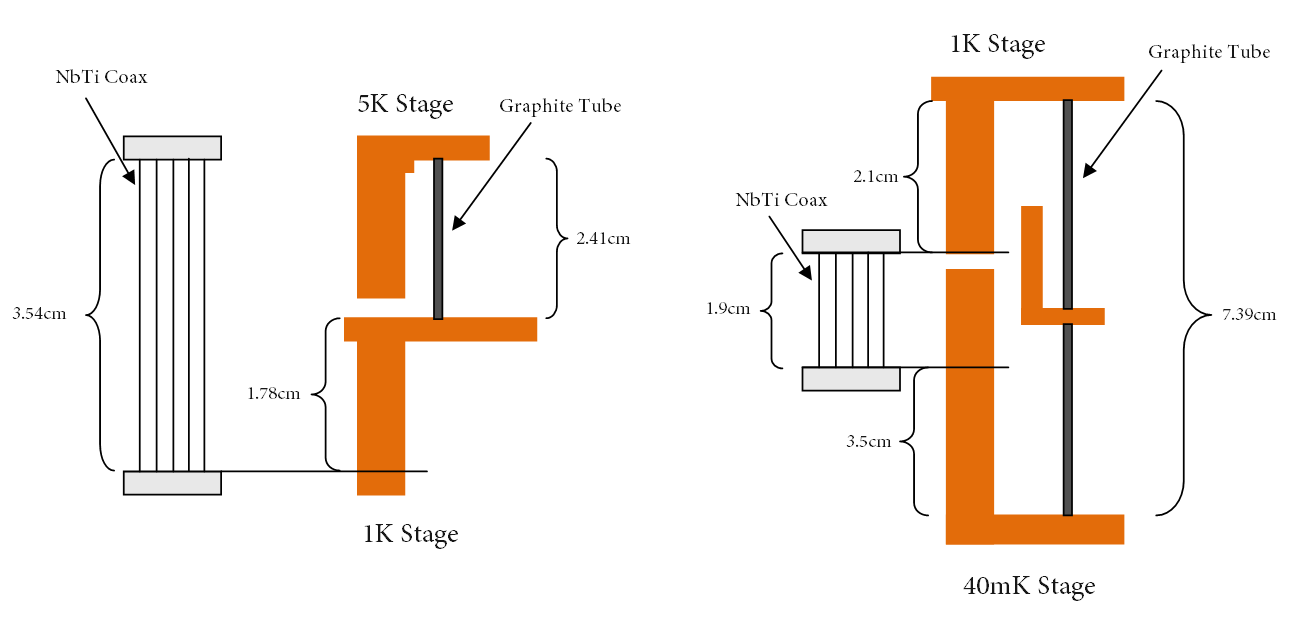
\includegraphics[width = \textwidth]{C:/Users/Niko/Documents/LaTex/Nick_K_Thesis/App_a_figs/Contraction_diagram.png}
\caption{The following model of the SuperCDMS Soudan towers was used in considering the relative contractions of the tower components. The 5K stage is the 4He-bath, the 1K stage is the Still, and the 40mK stage is the Mixing Chamber. The orange represents the OFHC copper tower.}
\end{figure}

The above tower model was used to determine the tensile stress on the side coaxes. These models consider the contiguous structure supporting the NbTi side coaxes, and its overall length change. This is compared to the contraction of the NbTi wires to determine strains. From here, material data gives us the stress in the coaxes.

\begin{figure}[h]
\centering
\begin{minipage}{.4\textwidth}
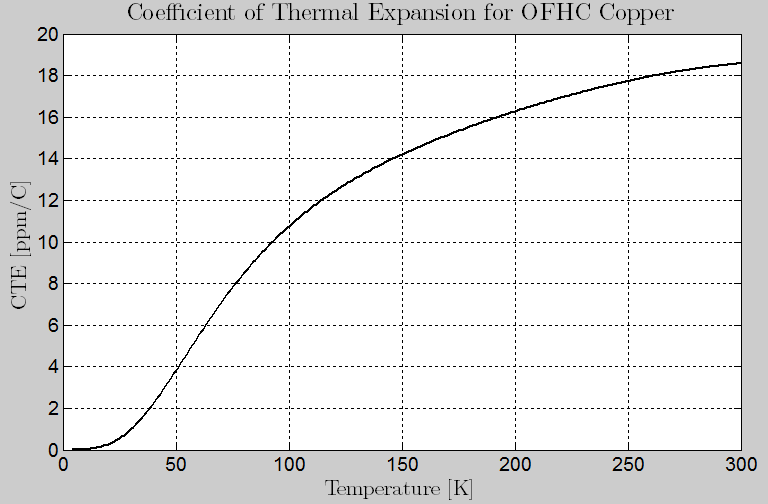
\includegraphics[width = \textwidth]{C:/Users/Niko/Documents/LaTex/Nick_K_Thesis/App_a_figs/CTE_ofhc_copper_plot.png}
\end{minipage}
\begin{minipage}{.4\textwidth}
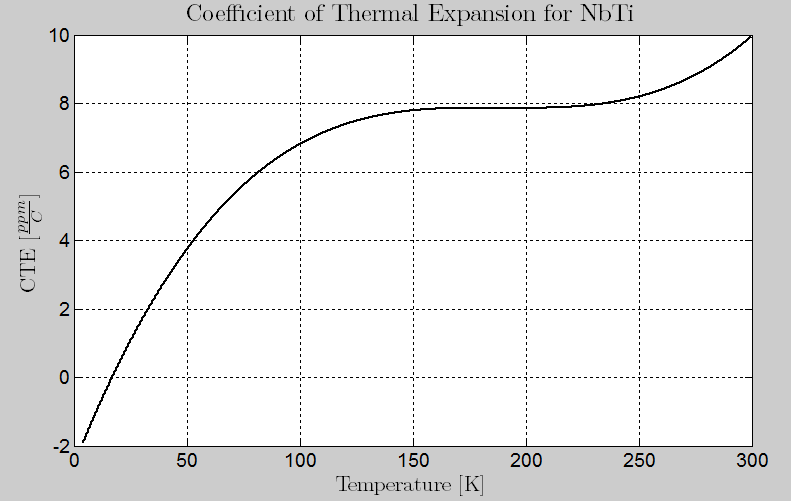
\includegraphics[width = \textwidth]{C:/Users/Niko/Documents/LaTex/Nick_K_Thesis/App_a_figs/CTE_nbti_plot.png}
\end{minipage}
\caption{Temperature-dependent Coefficient of thermal expansion for OFHC Copper \cite{ofhc_copper} and NbTi \cite{Marquardt2000}. The NbTi coefficient of thermal expansion was inferred from the formula for total contraction of NbTi, which explains its inaccuracy at very low temperatures. At higher temperatures, however, the curve is believable.}
\end{figure}

\section{Coefficients of Thermal Expansion}

To determine contraction, we need the thermal contraction characteristics of NbTi, OFHC Copper, and UF-4S graphite. Using NIST's property database \cite{ofhc_copper}, the temperature-dependent CTE of OFHC Copper was found. This is shown in Figure A.2.

The equation for the thermal contraction coefficient could then be integrated from 300K to 4K (the lowest data range for the equation) to approximate total fractional contraction from 300K to operating temperature. This is an approximation, as the temperature of the copper during operation is less than 4K, but gives negligible differences from reality.

The contraction of NbTi was found differently from copper. An equation for integrated thermal contraction was used, rather than one for just the coefficient. This equation reads,
\begin{eqnarray}
\frac{L_{T} - L_{293}}{L_{293}} = (a + bT + cT^2 + dT^3 + eT^4) \cdot 10^{-5}
\end{eqnarray}
\begin{table}[h]
\begin{tabular}{c}
a = -1.862E+02, b = -2.568E-01, c = 8.334E-03,  d = -2.951E-05, e = 3.908E-08\\
\end{tabular}
\end{table}

where a,b,c,d,e are a measured set of coefficients \cite{Marquardt2000}. This gives the fractional contraction from 293K to some T $\geq$ 4K. We used this formula to determine the temperature-dependent CTE for comparison to OFHC copper. This fractional contraction was plotted for temperatures between 4K and 293K. The slope between all points was then found, which gave the approximate temperature-dependent CTE at the temperature of the points. This is shown in Figure A.2 alongside copper.

The CTE for UF-4S graphite was obtained from a data sheet provided by Mersen, and is not given as a function of temperature. The CTE for UF-4S graphite is low, and depends on the grain orientation:
$$
CTE_{\parallel} = 1.8 \cdot 10^{-6}/C
$$
$$
CTE_{\perp} = 2.9 \cdot 10^{-6}/C
$$
where $CTE_{\parallel}$ is measured with the grain, and $CTE_{\perp}$ against the grain. The lower value of CTE is used in the calculations that follow to give conservative estimates.

\section{Tension from Fabrication}

The NbTi wires are soldered under tension to prevent loss of tension (and shorts) at operation temperature. This is done with two 30g weights - one hung at either end - for a total of 60g. Dividing by the cross-section of the wires, we get a stress of $805MPa$. The Modulus of Elasticity, $E$, for our Nb-47Ti (47\% Ti by weight) is $75.15GPa$. Using this, we get a strain of,
$$
Strain = \frac{Stress}{E} = \frac{75.15e9}{805e6} = 0.0107 \ or \ 1.07\%
$$

so the wires are strained 1.07\% beyond their equilibrium length.

\section{Stress on 5K - 1K Coax}

To calculate the stress on the NbTi wires, the strain was first calculated. Referring to Figure A.1, we see that the contiguous structure supporting the side coax consists of 2.41cm of graphite tube and 1.78cm of copper. The contraction of these will bring the ends of the wire closer together, decreasing strain. Conversely, the 3.54cm of NbTi wire will contract, acting to increase the strain. The third factor which comes into play is the tension created in the wire during the construction of the side coax. Combining all these effects, we calculate the wire length at 4K and compare it to the equilibrium length. This gives a strain which can be translated into a stress.

The strain is calculated from
\begin{eqnarray}
Strain = \frac{L - L_{eq}}{L_{eq}}
\end{eqnarray}
where $L$ is the actual length of the wires and $L_{eq}$ is the equilibrium length, both at 4K. We can see that
\begin{eqnarray}
L = L_{NbTi} - |\Delta L_{Cu}| - |\Delta L_{Tube}|
\end{eqnarray}
while,
\begin{eqnarray}
L_{eq \ 300K} & = & L_{NbTi} \cdot (1 - 0.0107) \\
L_{eq} & = & (L_{eq \ 300K})\cdot\left(1 - \left|\frac{\Delta L_{NbTi}}{L_{NbTi}}\right| \right)
\end{eqnarray}
where $\Delta L_{Cu}$ is the total contraction from 300K to 4K of the copper whose length is given in Figure A.1, $\Delta L_{Tube}$ is the graphite tube contraction, $\Delta L_{NbTi}/L_{NbTi}$ is the fractional NbTi contraction, $L_{NbTi}$ is the original length of the wires at 300K (3.54cm in this case), and $L_{eq \ 300K}$ is the equilibrium length at 300K. Putting these into the strain equation gives $1.05 \%$ strain. From this we find,
$$
Stress = E \cdot Strain = 75.15e9 \cdot 0.0105 = 791MPa
$$

\section{Stress on 1K - 40mK Span Coax}

The analysis carried out for the 1K - 40mK cable is similar to that for the 5K - 1K cable. For this cable, the contiguous support structure is more complicated. First, we have 7.39cm of graphite tube which will act to bring the wire ends closer together as they contract, decreasing strain. Second, we have the contracting copper. Due to the design of the tower (coax solder attachment points, etc.) we actually have $2.1cm + 3.5cm = 5.6cm$ of copper whose contraction will act to increase strain. Third, we have the contraction of the NbTi wires themselves, acting to increase the strain. Finally, we have the same applied tension as before, which creates a strain of 1.07\%.

The strain is again calculated with equation A.2. For this span, however, we will have,
\begin{eqnarray}
L = L_{NbTi} + |\Delta L_{Cu}| - |\Delta L_{Tube}|
\end{eqnarray}
where the sign change in front of $|\Delta L_{Cu}|$ reflects that copper contraction increases stage separation in this case. As before, we have,
\begin{eqnarray}
L_{eq \ 300K} = L_{NbTi} \cdot (1 - 0.0107) \\
L_{eq} = (L_{eq \ 300K})\cdot\left(1 - \left|\frac{\Delta L_{NbTi}}{L_{NbTi}}\right|\right)
\end{eqnarray}
with the same designations as before. Putting these into the strain equation gives $\approx 2.13 \%$ strain. This will be slightly less (about $2\%$) if the high CTE for graphite is used. From this we find,
$$
Stress = E \cdot Strain = 75.15e9 \cdot 0.0213 = 1604MPa
$$

This stress is much higher than the 5K - 1K coax stress. This is expected due to the short length of the wires for this span, as well as the large length of copper which is contracting. Though there is also a large length of graphite, its low CTE means it won't affect the total stress significantly.

\section{Acceptability of Stresses}

To see whether these loads are acceptable or not, we must know the yield strength for our NbTi alloy at base temperature. Our alloy, provided by Tekdata, is 47\% by weight Ti, which corresponds to 36.75\% \emph{Niobium} in atomic percentage. Yield strengths for similar alloys were found in the literature to range from 1230 MPa (34\% atm Nb, cold-worked) to 1750 MPa (39\% atm Nb, cold-worked and heat-treated) at 4.2K \cite{Collings1986}.

\begin{figure}[h]
\centering
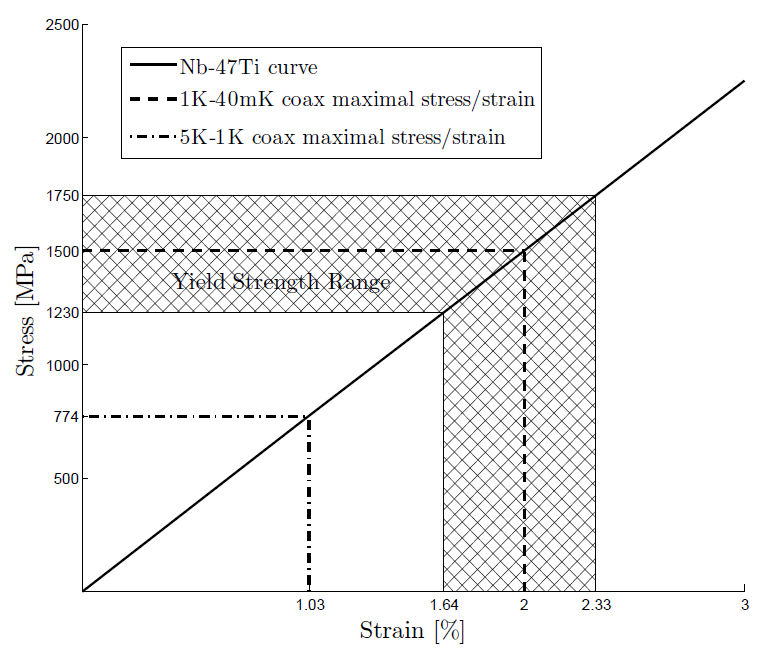
\includegraphics[width = .7\textwidth]{C:/Users/Niko/Documents/LaTex/Nick_K_Thesis/App_a_figs/NbTi_stress.png}
\caption{Stress v. Strain curve for Tekdata's Nb-47Ti (wt \%) alloy at room temperature. The maximal stresses/strains at base temperature are shown for the 5K-1K coax and 1K-40mK coax by a dot-dashed and a dashed line respectively. The range of yield strengths for similar alloys (and their corresponding strains) are given by the hatched region in the plot.  We see that the 1K-40mK line may be exceeding its yield strength at base. The alloys used were 34\% atm Nb, cold-worked (1230MPa) and 39\% atm Nb, cold-worked and heat-treated (1750 MPa) at 4.2K \cite{Collings1986}. Our alloy is 36.75\% \emph{Niobium} in atomic percentage.}
\end{figure}

The room temperature stress v. strain curve for our specific NbTi alloy is shown in Figure A.3. The range of yield strengths is shown in the hatched region. We see that the 5K - 1K coax is well below either yield strength; however, the 1K - 40mK coax stress falls well into the range for yield strengths of similar compositions.

To know for sure whether this is a real issue in our tower, we would need to 1), obtain the yield strength for our specific alloy/thermo-mechanical preparation and 2), find the young's modulus at low temperatures for our alloy. However, given that most materials tend toward a higher young's modulus at lower temperatures, there is a strong likelihood that this has been a problem in the Soudan towers.


\chapter{Thermal Conductivity Variation of Trace Materials}

Through a literature search and -- in some cases -- through testing, we have compiled thermal conductivities for candidate trace materials for the phonon cable. These thermal conductivities are shown to vary depending on the source of the material, its specific composition, and sometimes for unknown reasons (such as possible measurement error, natural material variation, etc.) The thermal conductivities of five candidate trace materials are presented here.
 
\begin{figure}[h]
\centering
\includegraphics[width=0.6\textwidth]{C:/Users/Niko/Documents/LaTex/Nick_K_Thesis/CH4_figs/mang_variation.png}
\caption{Thermal conductivity of Manganin wire by composition and author. There is little variation between data sets, suggesting a consistent, reproducible, thermal conductivity for Manganin wire.}
\end{figure}

\begin{figure}[h]
\centering
\includegraphics[width=0.6\textwidth]{C:/Users/Niko/Documents/LaTex/Nick_K_Thesis/CH4_figs/cuni_variation.png}
\caption{Thermal conductivity of Manganin wire by composition and author. There is little variation between data sets, suggesting a consistent, reproducible, thermal conductivity for Manganin wire.}
\end{figure}

\begin{figure}[h]
\centering
\includegraphics[width=0.6\textwidth]{C:/Users/Niko/Documents/LaTex/Nick_K_Thesis/CH4_figs/ss_variation.png}
\caption{Thermal conductivity of Manganin wire by composition and author. There is little variation between data sets, suggesting a consistent, reproducible, thermal conductivity for Manganin wire.}
\end{figure}

\begin{figure}[h]
\centering
\includegraphics[width=0.6\textwidth]{C:/Users/Niko/Documents/LaTex/Nick_K_Thesis/CH4_figs/ti153_variation.png}
\caption{Thermal conductivity of Manganin wire by composition and author. There is little variation between data sets, suggesting a consistent, reproducible, thermal conductivity for Manganin wire.}
\end{figure}

\begin{figure}[h]
\centering
\includegraphics[width=0.6\textwidth]{C:/Users/Niko/Documents/LaTex/Nick_K_Thesis/CH4_figs/nbti_variation.png}
\caption{Thermal conductivity of Manganin wire by composition and author. There is little variation between data sets, suggesting a consistent, reproducible, thermal conductivity for Manganin wire.}
\end{figure}


Thermal conductivity literature for trace material candidates. Variation between samples is largely due to varying thermo-mechanical treatment after production. In (b), Tekdata and Akerib measurements were performed on same wires used in CDMS Charge readout coaxes. In (d), Stainless alloys with similar composition to SS316 were used. Arrows indicate data sets used for graph in Section 1.2.



\chapter{Fluctuation in Resistance for Ti15-3-3-3 Trace}
The transition temperature of Ti 15-3-3-3 into its superconducting state is 3.89K \cite{wik}. If this material were used as a trace from the 4K stage to the Still of our towers, a portion of the trace would be in a normal state. This would give the line a resistance. Assuming the resistance of the line is low (tens of ohms), this is not a concern ; Fluctuating resistance, however, is a concern. As power loads to the fridge stages vary (from LED heating, circulation changes, etc.), the temperature gradient along the traces will vary as well. This will cause more/less of the line to be in a superconducting state -- varying resistance. The magnitude of these changes was calculated.

\begin{figure}[h]
\centering
\includegraphics[width = .5\textwidth]{Ti15333_trace_resistivity_section.png}
\caption{}
\end{figure}

\section{Determining the Temperature Profile for Ti 15-3-3-3 Traces}
The temperature profile along a Ti 15-3-3-3 trace was calculated, assuming steady-state planar heat flow. To do this, consider the trace in two sections -- one with length $l$ and the other with length $L-l$, where $L$ is the overall length of the trace, as shown in Figure 10. In steady-state, the power through these two sections will be equal, so
\begin{eqnarray}
\frac{A}{l}\int_{T}^{T_{high}} k(T)dT = P = \frac{A}{L - l}\int_{T_{low}}^{T} k(T)dT
\end{eqnarray}
where A is the cross-sectional area of the trace, $T_{high}$ and $T_{low}$ are the temperatures of the 4K stage and Still respectively, $T$ is the temperature at a length $l$ along the trace, and $k(T)$ is the thermal conductivity of the trace. After rearranging this becomes,
\begin{eqnarray}
\frac{l}{L-l} = \frac{\int_{T_{low}}^{T} k(T)dT}{\int_{T}^{T_{high}} k(T)dT}
\end{eqnarray}
which can be integrated to find the temperature at any point $l$ along the trace. Since the Ti 15-3-3-3 thermal conductivity had to be numerically integrated, T values were picked in $T \in [T_{low},T_{high}]$ and the corresponding $l$ values were found. Figure 11 shows the temperature profile for a 9.24cm trace with $T_{high} = 4.2K$ and $T_{low}=0.6K$.

\begin{figure}[h]
\centering
\includegraphics[width = .5\textwidth]{Ti153_T_Profile.png}
\caption{}
\end{figure}

\section{Resistivity of Ti 15-3-3-3}
The resistance of Ti 15-3-3-3 was measured by P. Wikus et al. Using the given dimensions, we converted to resistivity. This was then fitted to an equation to enable us to find the resistivity of Ti 15-3-3-3 as a function of temperature. The fitted resistivity is shown in Figure 12.

\begin{figure}[h]
\centering
\includegraphics[width = .6\textwidth]{Ti_Resistivity.png}
\caption{Resistivity of Ti 15-3-3-3 showing $T_c$ at 3.89K}
\end{figure}

\section{Total Resistance of Trace}

Combining the resistivity and temperature profiles, the trace was subdivided into sections, each assigned a length, and the resistance was calculated for each. From this, the total resistance of the line was calculated. We find,

\begin{table}[h]
\begin{threeparttable}
\begin{tabular}{lcr}
\toprule
\multicolumn{2}{r}{Total Resistance [$\Omega$]} \\
\midrule
5K - 1K & $\rightarrow$ & 13.60 \\
4.2K - 0.6K & $\rightarrow$ & 5.64 \\
\bottomrule
\end{tabular}
\end{threeparttable}
\end{table}

\noindent With a total fluctuation of \bf{7.96 $\Omega$}.


\restoregeometry

\chapter{Aluminum as a Candidate Trace Material}

Aluminum is naturally under consideration as a trace material, due to its well known properties and widespread use. Fabrication time for a stripline would be reduced by using Aluminum, as the company fabricating the line, Tech-Etch, has used it as a trace material in the past. A new material, such as Ti15-3-3-3 would require significantly more time to go through the development process. Therefore, it is in our best interest to examine the feasibility of an Aluminum-trace stripline. Considerations for its suitability include its thermal conductivity, coefficient of thermal expansion (CTE), and critical temperature ($T_{c}$).

\section{Thermal Conductivity of Al5056}

The Aluminum used by Tech-Etch is 5052-H19, however members of our collaboration were unable to find low temperature thermal conductivity data for this alloy. The thermal conductivity of another alloy, Al5056, was found to be very similar in normal state, so was used a proxy for 5052-H19. The thermal conductivity of Al5056 was determined from \cite{coc} for the range 600mK down to 50mK as,
\begin{equation}
K(T) = 1.9 \cdot 10^{4} T^{2.83} \mu W/cmK
\end{equation}

This thermal conductivity is compared to other phonon stripline candidate materials in Figure 4 below. In the range of interest (600mK - 50mK) we can see that the thermal conductivity of Al5056 is almost two orders of magnitude higher than NbTi and Ti15-3-3-3.

\begin{figure}[h]
\includegraphics[width = .87\textwidth]{Cable_Therm_Graph.png}
\caption{Thermal conductivities of various stripline candidate materials. The thermal conductivity of Al5056 is nearly two orders of magnitude higher than NbTi or Ti15-3-3-3}
\end{figure}


\section{Aluminum Heat Load}

To see if Al will work as a trace material, the thermal power conducted from 600mK to 50mK must be within our thermal budget for the 50mK still of our fridge. The power conducted between a thermal gradient is given by equation 1 in the report. Using a thickness of 1 mil, width of 40 mils, and a trace length of 0.79 inches we can calculate the power for each trace. Assuming 16 traces per detector and 6 detectors per tower, as well as accounting for Kapton heat load, we are able to estimate the total flex cable heat load per tower. The loads for Al5056 are compared with other trace materials in table 7.


\begin{table}
\begin{threeparttable}
\begin{tabular}{l|c|r}
\toprule
Material & Power/Trace [nW] & Total Load per Tower [nW] \\
\midrule
Ti 15-3-3-3 & 0.85 & 684 \\
NbTi & 1.4 & 739 \\
Aluminum & 92 & 9471 \\
\bottomrule
\end{tabular}
\end{threeparttable}
\caption{Estimated heat load for an Aluminum-trace flex cable from 600mK to 50mK as compared with other candidate materials. Assumes 1 mil thick, 40 mils wide, 0.79 inch long traces; 16 traces per detector and 6 detectors per tower.}
\end{table}

The thermal budget for the 50mK end (the still) is $\sim 1 \mu W$. The Al5056 trace heat load is an estimated $9.5 \mu W$ per tower. The heat load for one tower is higher than the thermal budget, though our experiment necessitates the use of multiple towers. Reducing the width of the traces, as well as lengthening the traces could reduce this to perhaps $1\mu W$ (still too high), but inductance constraints would significantly complicate the design.


\section{Thermal Expansion Coefficient of Aluminum}
It is important to match the expansion coefficients of materials which will undergo large temperature changes. In our flex cable, we will be epoxy-ing the Aluminum traces to Kapton polyimide, so the CTE of these two materials should match relatively well. The linear coefficient of thermal expansion presented for Aluminum is 24ppm/K while DuPont states the coefficient for Kapton HN to be 20ppm/K. These values are well matched, so in this regard, Aluminum suites our needs.

\section{Critical Temperature}

The trace material for our striplines must be in a superconducting state for the temperatures at which they are used. The alloy used by Tech-Etch, 5052-H19, has a $T_{c}$ of 775mK. This low $T_{C}$ limits the alloy's use to the 600mK - 50mK span of our flex cable, as it would be in a normal state for most of the 4.2K - 600mK span. The low $T_{c}$ of the alloy is a concern, due to non-ideal temperatures in our fridge. If the temperature drifts upward past the $T_{c}$ of the Aluminum, then the traces will transition to a normal state. Fridge temperatures have been to drift up to as much as 1K, so this is a serious concern for the feasibility of an Aluminum-trace stripline.

\section{Conclusion}

Due to the high thermal conductivity of Aluminum, and the resulting heat load, as well as the low $T_{c}$, our collaboration has decided that it is unsuitable as a trace material.

\end{appendices}

\newpage
\bibliography{C:/Users/Niko/Documents/LaTex/Bibliographies/thesis}

\end{document}
